\documentclass[12pt,a4paper]{ctexart}
\usepackage{ctex}
\usepackage{fontspec}    % 字体设置包  
\usepackage{graphicx}    % 插入图片
\usepackage{amsmath}     % 数学公式
\usepackage{amssymb}     % 数学符号
\usepackage{geometry}    % 页面布局
\usepackage{titlesec}    % 标题格式
\usepackage{enumitem}    % 列表设置
\usepackage{lipsum}      % 生成示例文本
\usepackage{unicode-math}
\usepackage{longtable}
% 基础图片插入包
\usepackage{graphicx}
% 子图标题与编号包(推荐,功能更全)
\usepackage{subcaption}
% (可选)调整图片与文字间距
\usepackage{float}
\usepackage{booktabs}
\usepackage{multirow}   % 用于合并单元格
\usepackage{multicol}   % 支持多栏布局(此处用于外层分栏)
% 页面设置
\geometry{margin=1.5in}  % 页边距



% 标题格式设置
%\titleformat{\section}{\centering\Large\bfseries}{\thesection}{1em}{}
%\titleformat{\subsection}{\large\bfseries}{\thesubsection}{1em}{}

% 标题信息
\title{探究不同材质杯子在不同液体残留下的最佳清洗频率}
\author{董柏霖,张展搏,孙敏涵}
\date{\today}  % 使用当前日期

\begin{document}

\maketitle  % 生成标题

\begin{abstract}
水杯清洁不当易引发微生物污染,可重复使用水瓶细菌菌落数常达千万级 CFU,但公众对水杯清洁与使用的认知缺乏科学依据。本研究以不锈钢片、陶瓷片模拟水杯材质,无菌水、乌龙茶、沁葡水为实验液体,通过 1-5 天时间梯度培养,结合偏置修正、函数拟合及数据归一化处理,分析微生物生长规律。
实验结果显示:不锈钢抑菌性优于陶瓷,尤其适配含糖饮料;乌龙茶因含茶多酚抑菌,长期放置带菌量最低,沁葡水长期带菌量暴增;短期宜用灭菌水,长期茶类更优。

我们得出结论:无菌水可任意选杯,含糖饮料优选不锈钢杯且不宜久放,茶类适配陶瓷杯。研究创新采用材质薄片实验与偏置数据处理法,未来需优化变量控制与样本量,为饮水卫生及水杯制造提供参考 。
\end{abstract}
\newpage
\tableofcontents
\newpage

\section{引言}
\subsection{实验背景}

在日常生活中,我们常听到“不要喝隔夜水”的建议,也屡见媒体报道因水杯清洁不当引发的卫生问题。例如,2025年1月6日,美国净水器制造商Water Filter Guru发布的一项调查显示,如果未能认真清洗,一个可重复使用的水瓶中平均可检出2080万个细菌菌落形成单位(CFU),约为电脑鼠标细菌数量的5倍;其中带有运动壶嘴的水瓶菌落数甚至可高达3000万CFU,污染程度可能超过马桶座圈。这一数据突显了日常饮水容器中微生物污染的严重性与潜在健康风险。

饮用容器使用后放置,内壁易残留水分、有机物及微生物,形成生物膜,成为细菌、霉菌等滋生的温床。尤其在常温环境下,某些材质的杯体表面更易附着和积累微生物,增加饮用者发生肠道感染或其他健康问题的概率。目前,公众对水杯清洁频率、材质选择及盛放液体类型的影响仍缺乏科学、系统的认知,相关行为多基于经验或习惯,亟须通过实验研究提供理论依据与实践指导。

\subsection{实验目标}

本研究旨在通过模拟日常使用条件,对不同材质水杯(不锈钢、陶瓷)中微生物的生长规律进行定性、定量分析,明确其菌落数量随时间的变化情况,进而确定合理的清洗周期;同时,比较不同材质表面对微生物吸附及增殖的影响,为选择安全性更高的水杯材料提供依据;此外,还将探讨常见饮品(如清水、茶、糖饮料等)对微生物生长的影响。通过上述研究,我们希望建立科学的水杯使用与清洁策略,从源头上减少因细菌污染导致的健康风险,提升公众日常饮水卫生水平。


\section{材料与方法}
\subsection{材料与试剂}
\begin{longtable}{lll}  % 三列均为左对齐(l),与原表格格式一致
  \caption{实验材料参数及用途表} \label{tab:material} \\  % 表格标题与标签
  \toprule  % 三线表顶部粗线(顶线)
  \textbf{材料} & \textbf{参数} & \textbf{用途} \\  % 表头(加粗突出)
  \midrule  % 三线表中间细线(表头线)
  \endfirsthead  % 首页表头结束标志

  \caption*{表 \ref{tab:material}(续):实验材料参数及用途表} \\  % 后续页续表标题
  \toprule
  \textbf{材料} & \textbf{参数} & \textbf{用途} \\
  \midrule
  \endhead  % 后续页表头结束标志

  \bottomrule  % 每页页尾底线(暂存,末页会覆盖)
  \multicolumn{3}{r}{(续表)} \\  % 页尾右侧标注“续表”
  \endfoot  % 页尾内容结束标志

  \bottomrule  % 末页底部粗线(最终底线)
  \endlastfoot  % 末页页尾结束标志

  % 表格核心内容(与原表格完全一致)
  不锈钢片             & $20 \times 20 \times 2\ \mathrm{mm}$ & 菌落附着材料 \\
  陶瓷片               & $20 \times 20 \times 2\ \mathrm{mm}$ & 菌落附着材料 \\
  无菌水               & /                                   & 实验液体     \\
  乌龙茶               & /                                   & 实验液体     \\
  沁葡水               & /                                   & 实验液体     \\
  牛肉膏蛋白胨培养基   & 牛肉膏蛋白胨培养基                   & 配置培养基   \\
\end{longtable}

\subsection{实验方法}
实验前,将乌龙茶、沁葡水及无菌水分装于若干小锥形瓶中,陶瓷片与不锈钢片以报纸包裹,连同培养皿、小试管等实验器材经高压蒸汽灭菌后转移至无菌室。同时配制1 L牛肉膏蛋白胨培养基,装于锥形瓶中灭菌后,于无菌室内分装至培养皿并密封,避免污染。

\subsubsection{样品处理与培养条件设置}

为模拟杯壁液体残留情形,在无菌室内对操作环境及实验者进行酒精消毒后,将灭菌后的材质薄片置于无菌培养皿中。使用移液枪精准量取三种液体各1 mL,分别滴加于不锈钢片和陶瓷片表面,并标注材质、液体类型与放置时间(如:不锈钢-水-1天)。每种材质与液体的组合均设置5个时间梯度(1、2、3、4、5天),以获取连续时间段的微生物生长数据。将沾有不同液体的不锈钢片和陶瓷片样品置于相同室温阴凉环境中,模拟未彻底清洗的容器表面残留液体的真实环境。

\subsubsection{微生物回收与培养}

到达预定时间后,将样品密封带回无菌室,使用经酒精灼烧并冷却的镊子取样品薄片,置入装有10mL无菌水的小试管中搅拌,制备原液。随后进行10倍系列梯度稀释,每个稀释度取500 µL菌液涂布于牛肉膏蛋白胨平板,每个样品做三个平行,确保实验数据的准确性。涂布后的平板置于恒温培养箱中,于37℃下培养一周。

\subsubsection{数据初步收集}

培养结束后,对平板上生长的菌落进行拍照记录,进行菌落计数与形态学初步鉴定,以统计不同条件下的微生物残留量。


\subsection{数据处理方法}

\subsubsection{数据清洗}
在我们获取的数据中,包含许多异常数据与缺失值,我们主要采用添加偏置的方法修正一组异常项;同时使用函数拟合的方式填补缺失值。
\paragraph{偏置项}
由于本实验分批次完成(1-2天一组,3-5天一组),故每一组的初始条件(初始菌落数)不同,对于3-5天这组,我们会通过对其添加偏置项来修正它的初始菌落数目,从而得出较为合理的数据。


即对于某一组菌落数据${x}={x_1,x_2,x_3,x_4,x_5}$,经过修正后的数据则表示为:$x_{cor}=x_1,x_2,x_3+\theta,x_4+\theta,x_5+\theta $($\theta$ 为偏置项)

大部分偏置项的确定依赖于1-2天(即正常组)的培养情况,确保在调整后图像光滑;

%\paragraph{函数拟合}
%由于缺少部分数据,导致我们只能通过函数拟合的方式预测可能的缺失数据。而由于缺失数据周围有正常数据,所以拟合的结果具有一定的可信度。

%对于铁片组数据有如下函数(x代表天数,y代表带菌量):
%\begin{enumerate}
    %\item 铁片-无菌水:$ y = 100.43x^2 - 240.36x + 203.13$
    %\item 铁片-沁葡水:$y = 29.35 \times e^{0.96x}$,以第3天为$x=0$
    %\item 铁片-乌龙茶:$y = 352 \times e^{-0.64 \times (x-2)} $(以第2天为起点开始衰减)
%\end{enumerate}

\subsubsection{数据预处理}
为了分析的简便,我们事先对数据进行了预处理,主要是对数据进行Min-Max 归一化,将数据线性映射到$[0,1]$空间内。公式表达为:
\begin{equation}
    \hat{x}=\frac{x−min(X)​}{max(X)−min(X)},\hat{x} \in [0,1]
\end{equation}
其中,$\hat{x}$表示归一化后的数据,$X$为同种材料、同种饮料的数据集。
\section{实验结果}
在此板块中,我们定义一些时间跨度来更准确简便地描述实验结果:
\begin{itemize}
    \item 初期:1-2天
    \item 中期:2-3天
    \item 长期:4-5天
\end{itemize}
\subsection{放置天数以及承装液体种类对同种材料的影响}
\subsubsection{不锈钢片}
\paragraph{控制天数相同,而承装液体不同}
\begin{figure}[htbp]  % htbp:浮动体位置优先级(here, top, bottom, page)
    \centering  % 整体居中
    % 子图1:宽度占页面的1/3,减去间距(避免溢出)
    \begin{subfigure}[b]{0.31\textwidth}  % [b]:子图标题底部对齐;0.31\textwidth:子图宽度
        \centering
        % 插入图片:width=\linewidth 表示图片宽度=子图环境宽度
        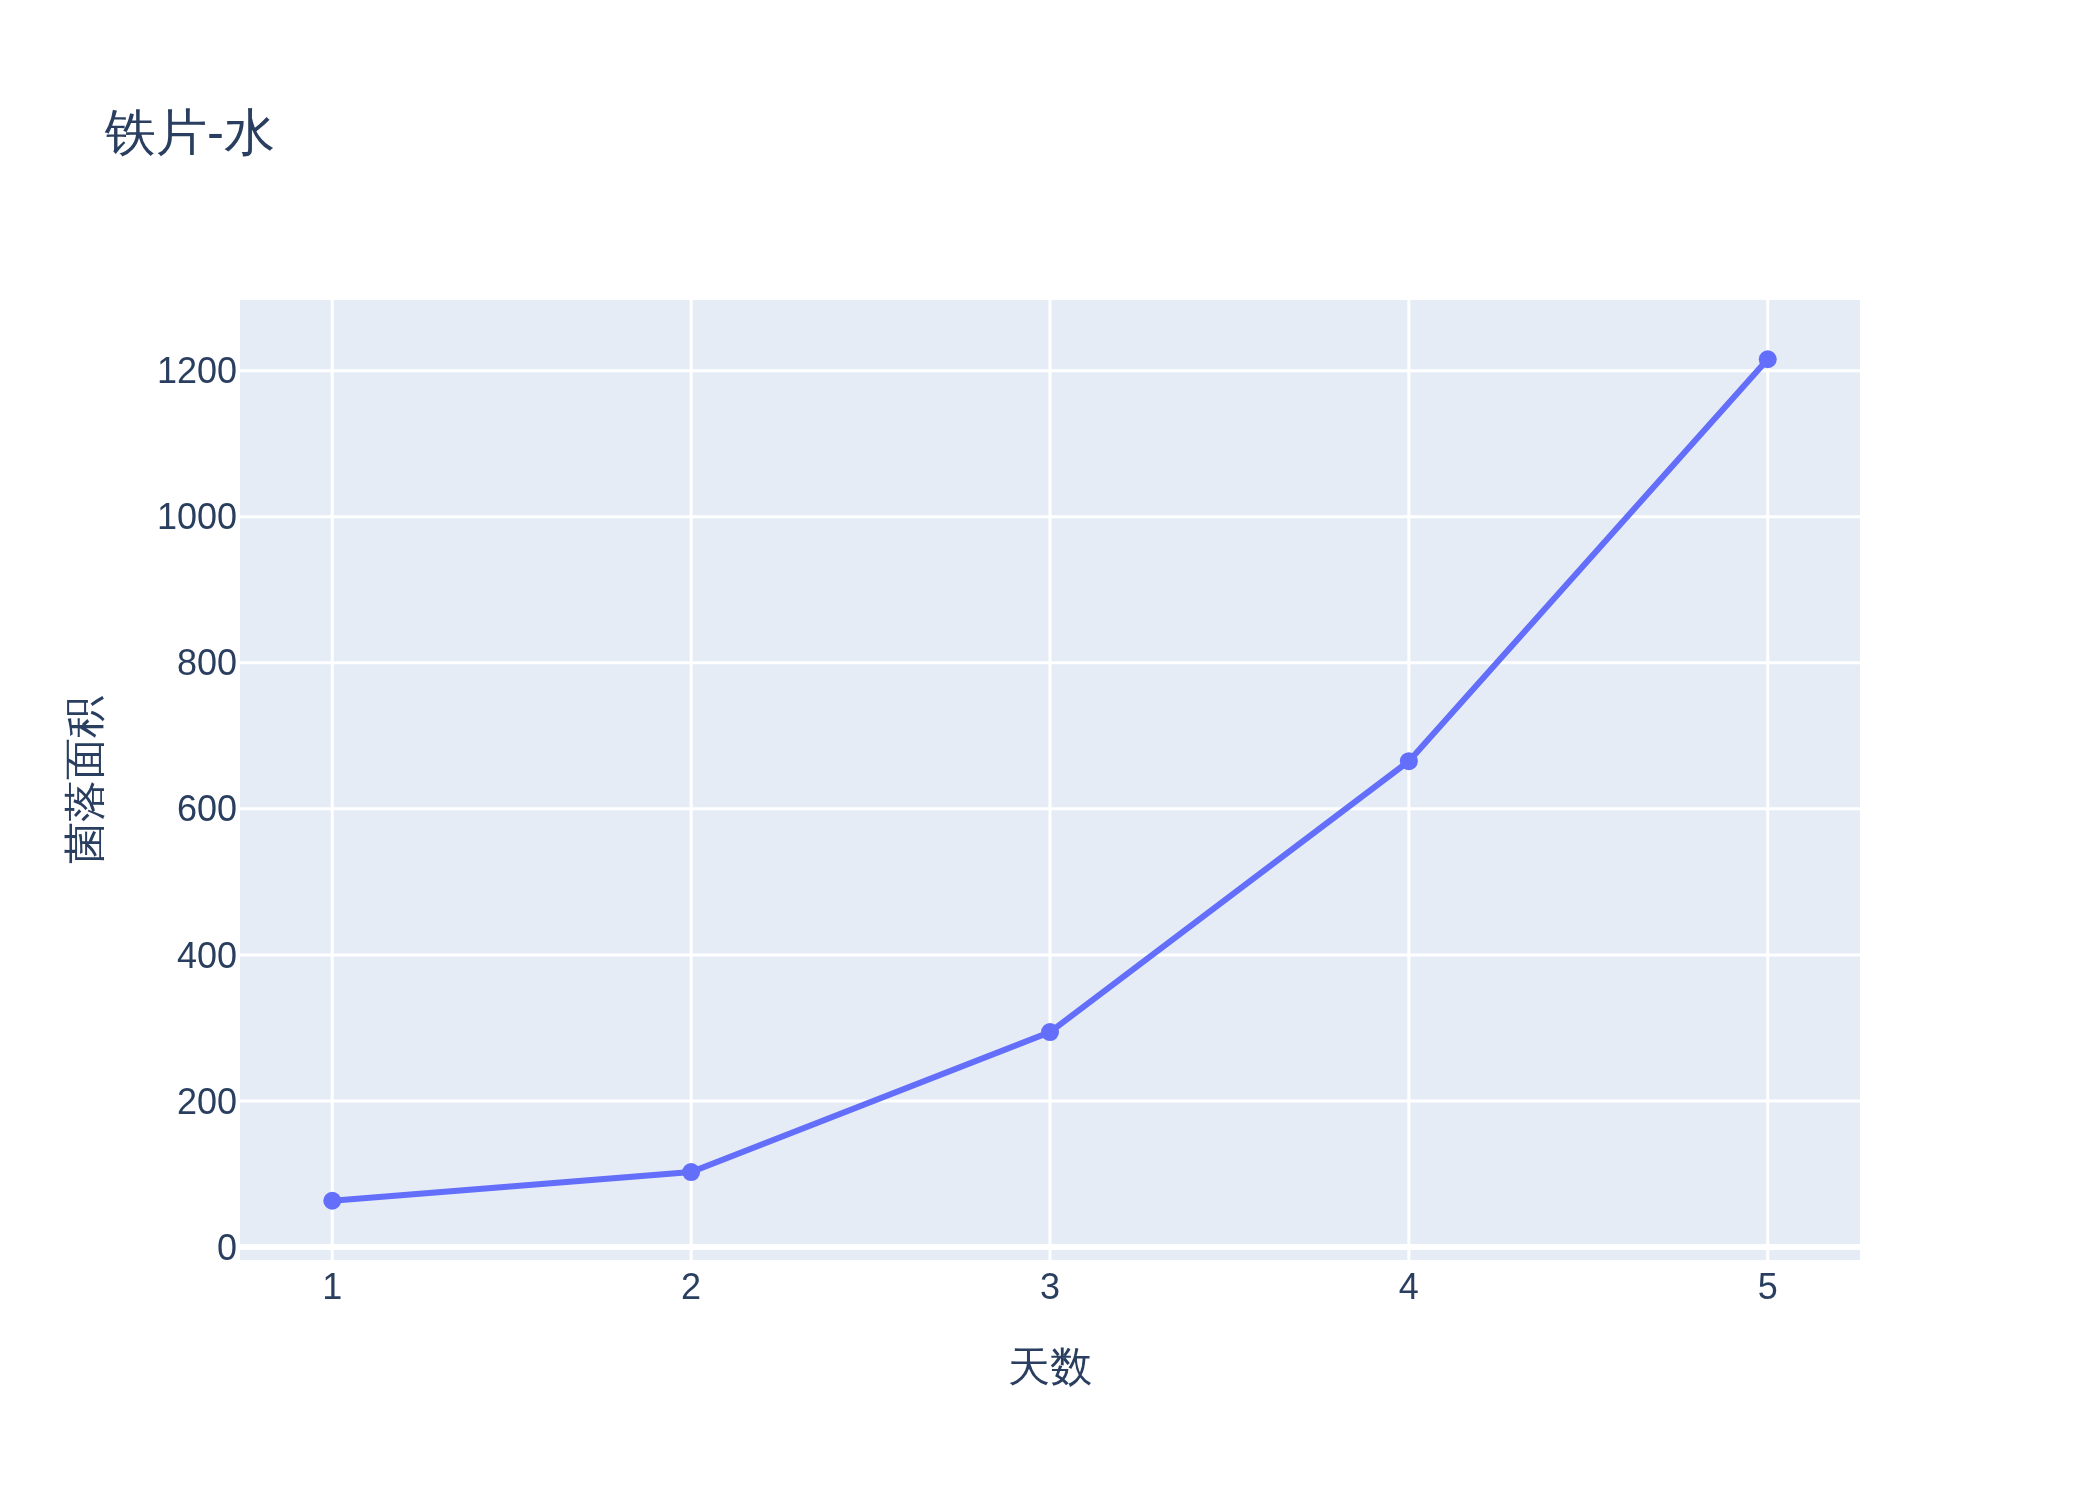
\includegraphics[width=\linewidth]{./plot/SingleMaterial/iron/铁片-水_line.png}  % 替换为你的图片路径/文件名
        \caption{不锈钢片-水}  % 子图1的标题
        \label{subfig:1}     % 子图1的引用标签(用于后文交叉引用)
    \end{subfigure}
    \hfill  % 子图间水平填充空白(均匀分布)
    % 子图2:与子图1宽度一致
    \begin{subfigure}[b]{0.31\textwidth}
        \centering
        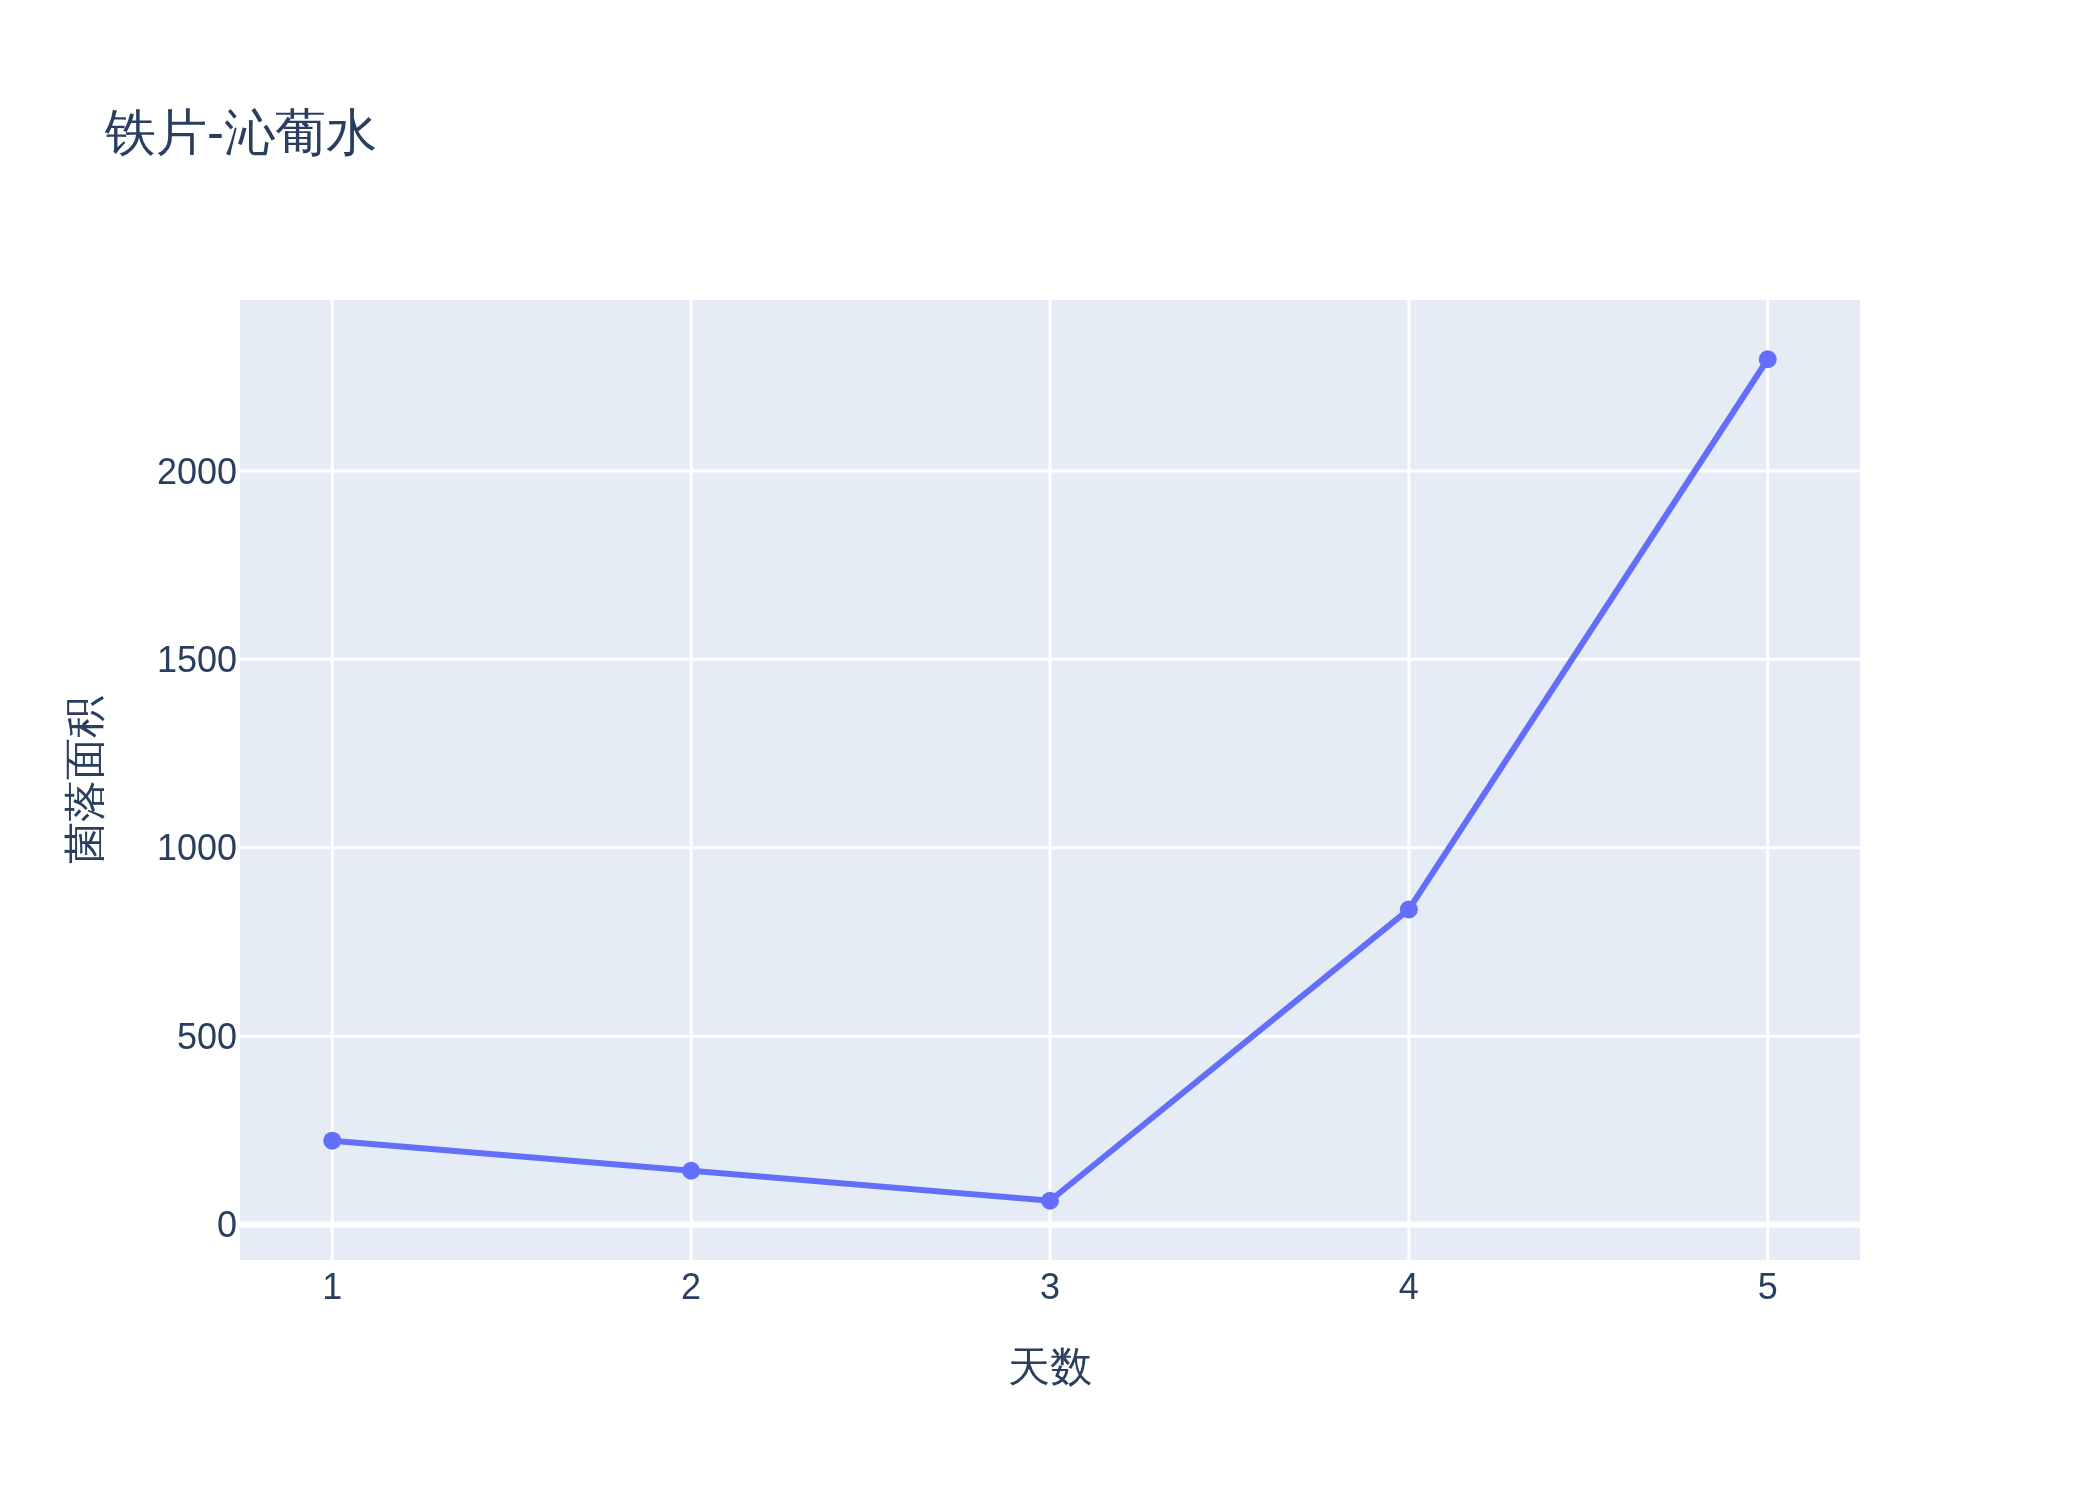
\includegraphics[width=\linewidth]{./plot/SingleMaterial/iron/铁片-沁葡水_line.png}
        \caption{不锈钢片-沁葡水}
        \label{subfig:2}
    \end{subfigure}
    \hfill  % 再次填充空白
    % 子图3:与前两个子图宽度一致
    \begin{subfigure}[b]{0.31\textwidth}
        \centering
        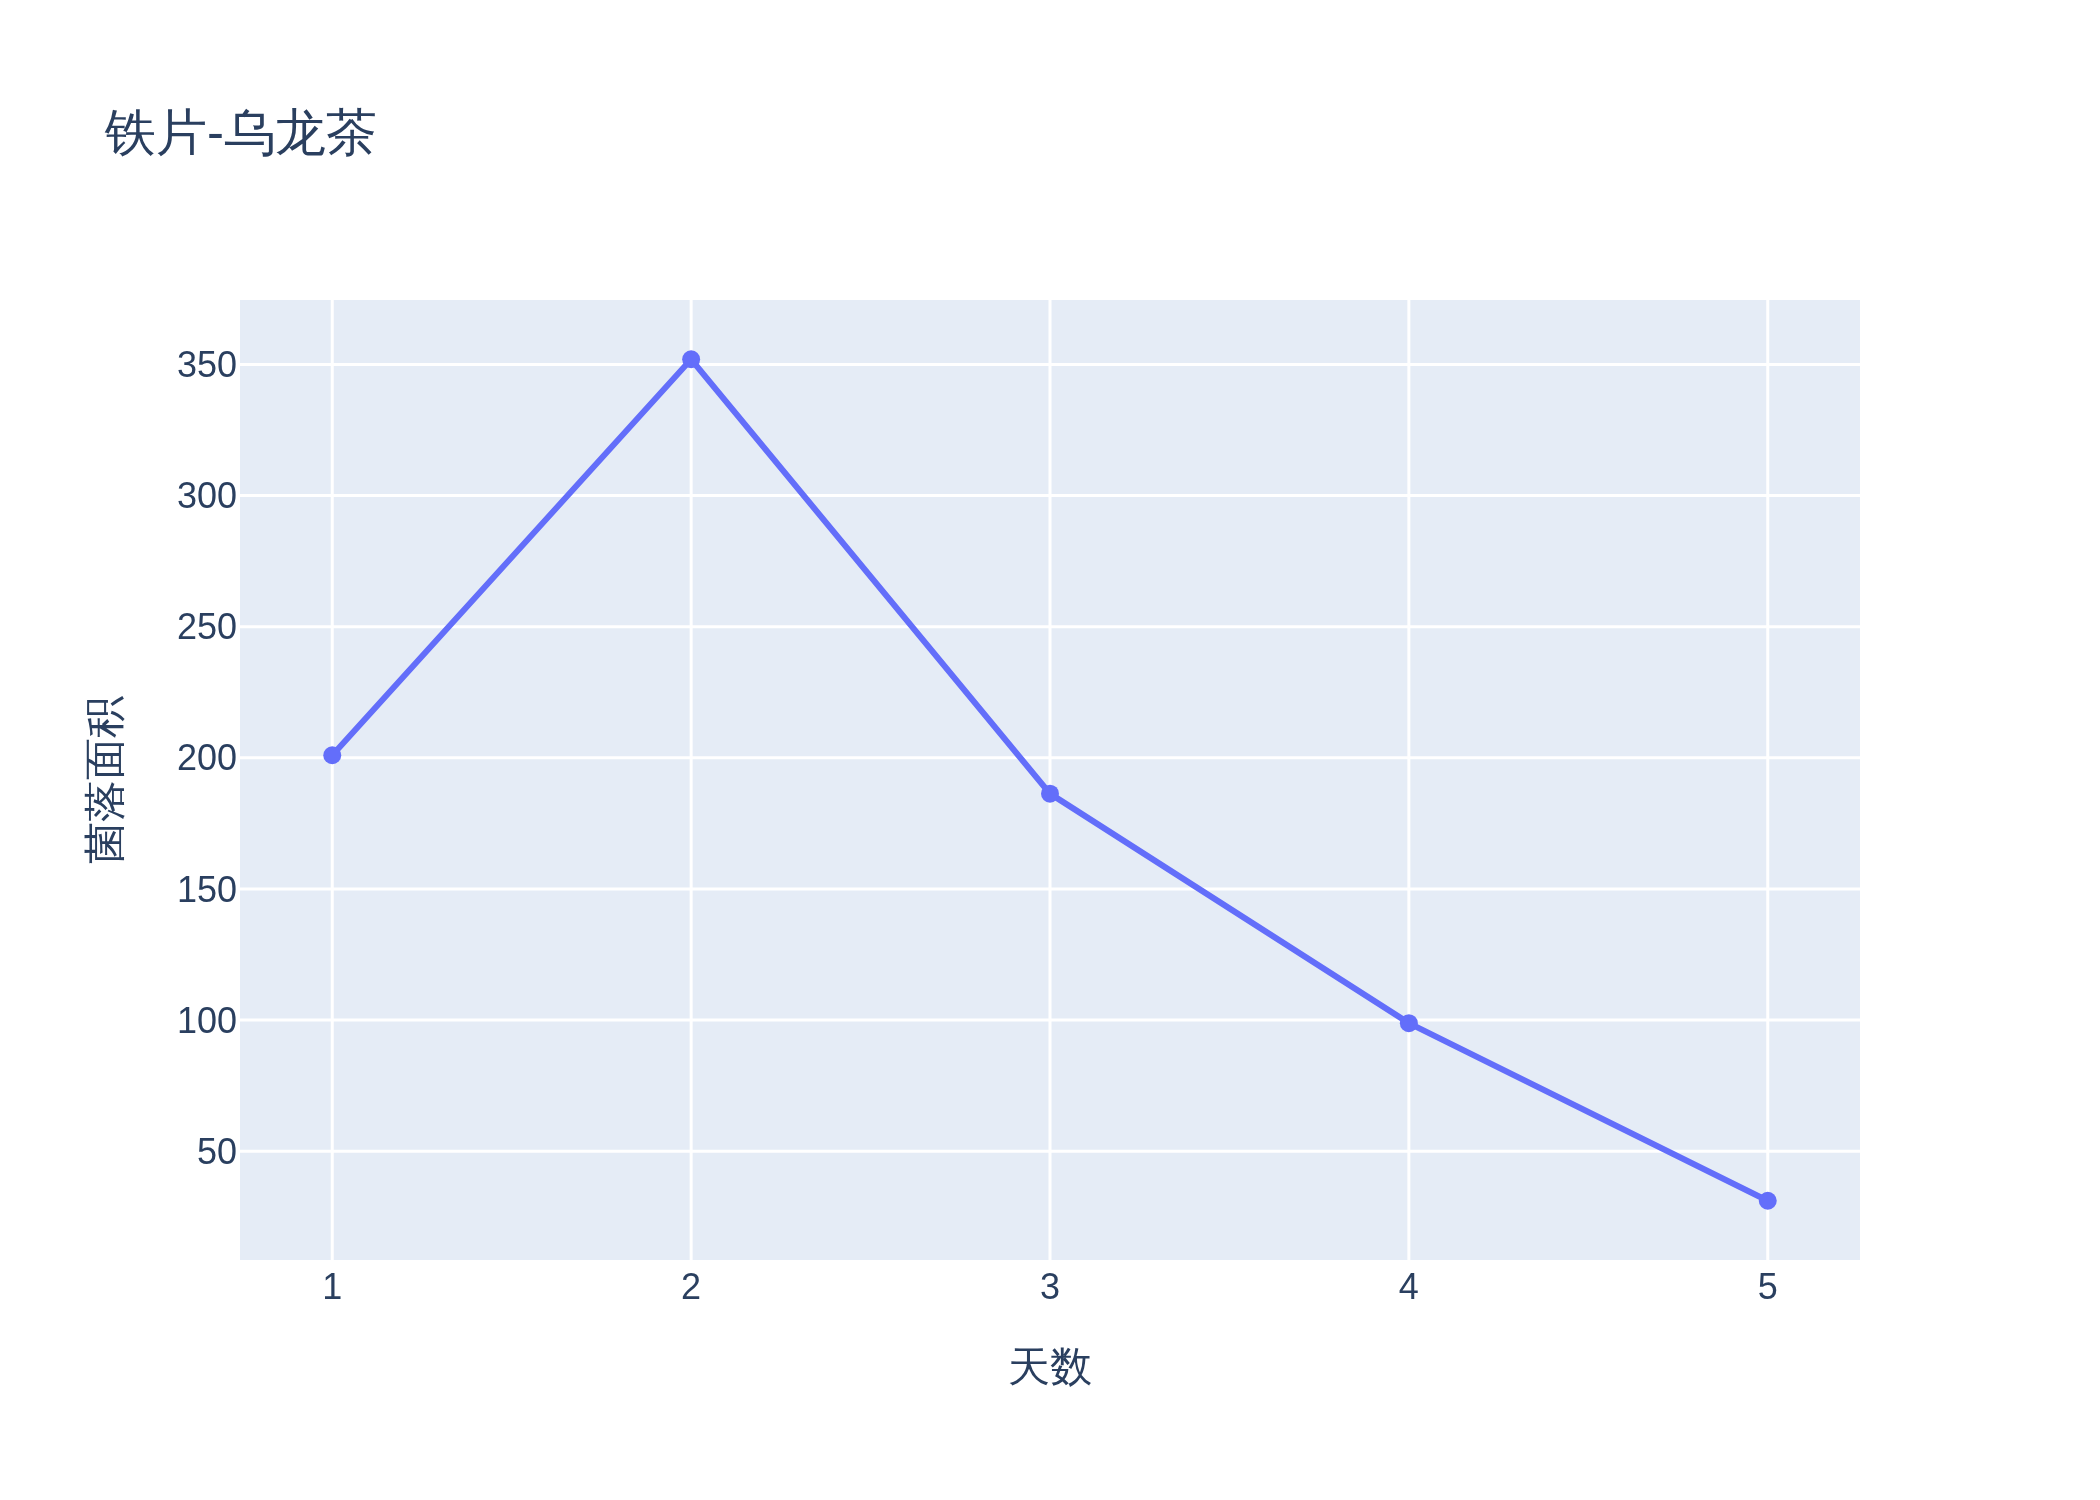
\includegraphics[width=\linewidth]{./plot/SingleMaterial/iron/铁片-乌龙茶_line.png}
        \caption{不锈钢片-乌龙茶}
        \label{subfig:3}
    \end{subfigure}
    % 整个三联图的总标题
    \caption{不锈钢片在3种溶液下表面的微生物情况}
    \label{fig:triple_horizontal}  % 整个图的引用标签
\end{figure}
\begin{itemize}
    \item 初期无菌水组带菌量较少,而乌龙茶、沁葡水带菌量均较高。
    \item 中期沁葡水组、乌龙茶组带菌量出现降低,水组持续升高。但由于沁葡水的异常降低,乌龙茶带菌量最大,水次之,沁葡水最小。
    \item 长期乌龙茶组带菌量持续减低,而沁葡水组暴增,水组数据缺失。沁葡水带菌量最多,无菌水次之,乌龙茶最小。
\end{itemize}







\paragraph{控制承装液体相同,天数不同,可以得到:}
\begin{enumerate}
    \item 无菌水组:起始低,带菌量随天数持续增长,且增幅持续变大。
    \item 沁葡水组:起始高,带菌量随天数有短期下降,但大体上升,在长期中会突增。
    \item 乌龙茶组:起始较高,带菌量随天数持续下降。
\end{enumerate}
\subparagraph{总结}
结合数据,我们不难得到,对于用不锈钢杯子1到2天的承装,盛开水,这种经过高压杀菌过的水在微生物的含量上最少,而长期承装肯定是具有抑菌性能的茶类比较适合。

\subsubsection{陶瓷片}
\subparagraph{控制天数相同,而承装液体不同}
\begin{figure}[htbp]  % htbp:浮动体位置优先级(here, top, bottom, page)
    \centering  % 整体居中
    % 子图1:宽度占页面的1/3,减去间距(避免溢出)
    \begin{subfigure}[b]{0.31\textwidth}  % [b]:子图标题底部对齐;0.31\textwidth:子图宽度
        \centering
        % 插入图片:width=\linewidth 表示图片宽度=子图环境宽度
        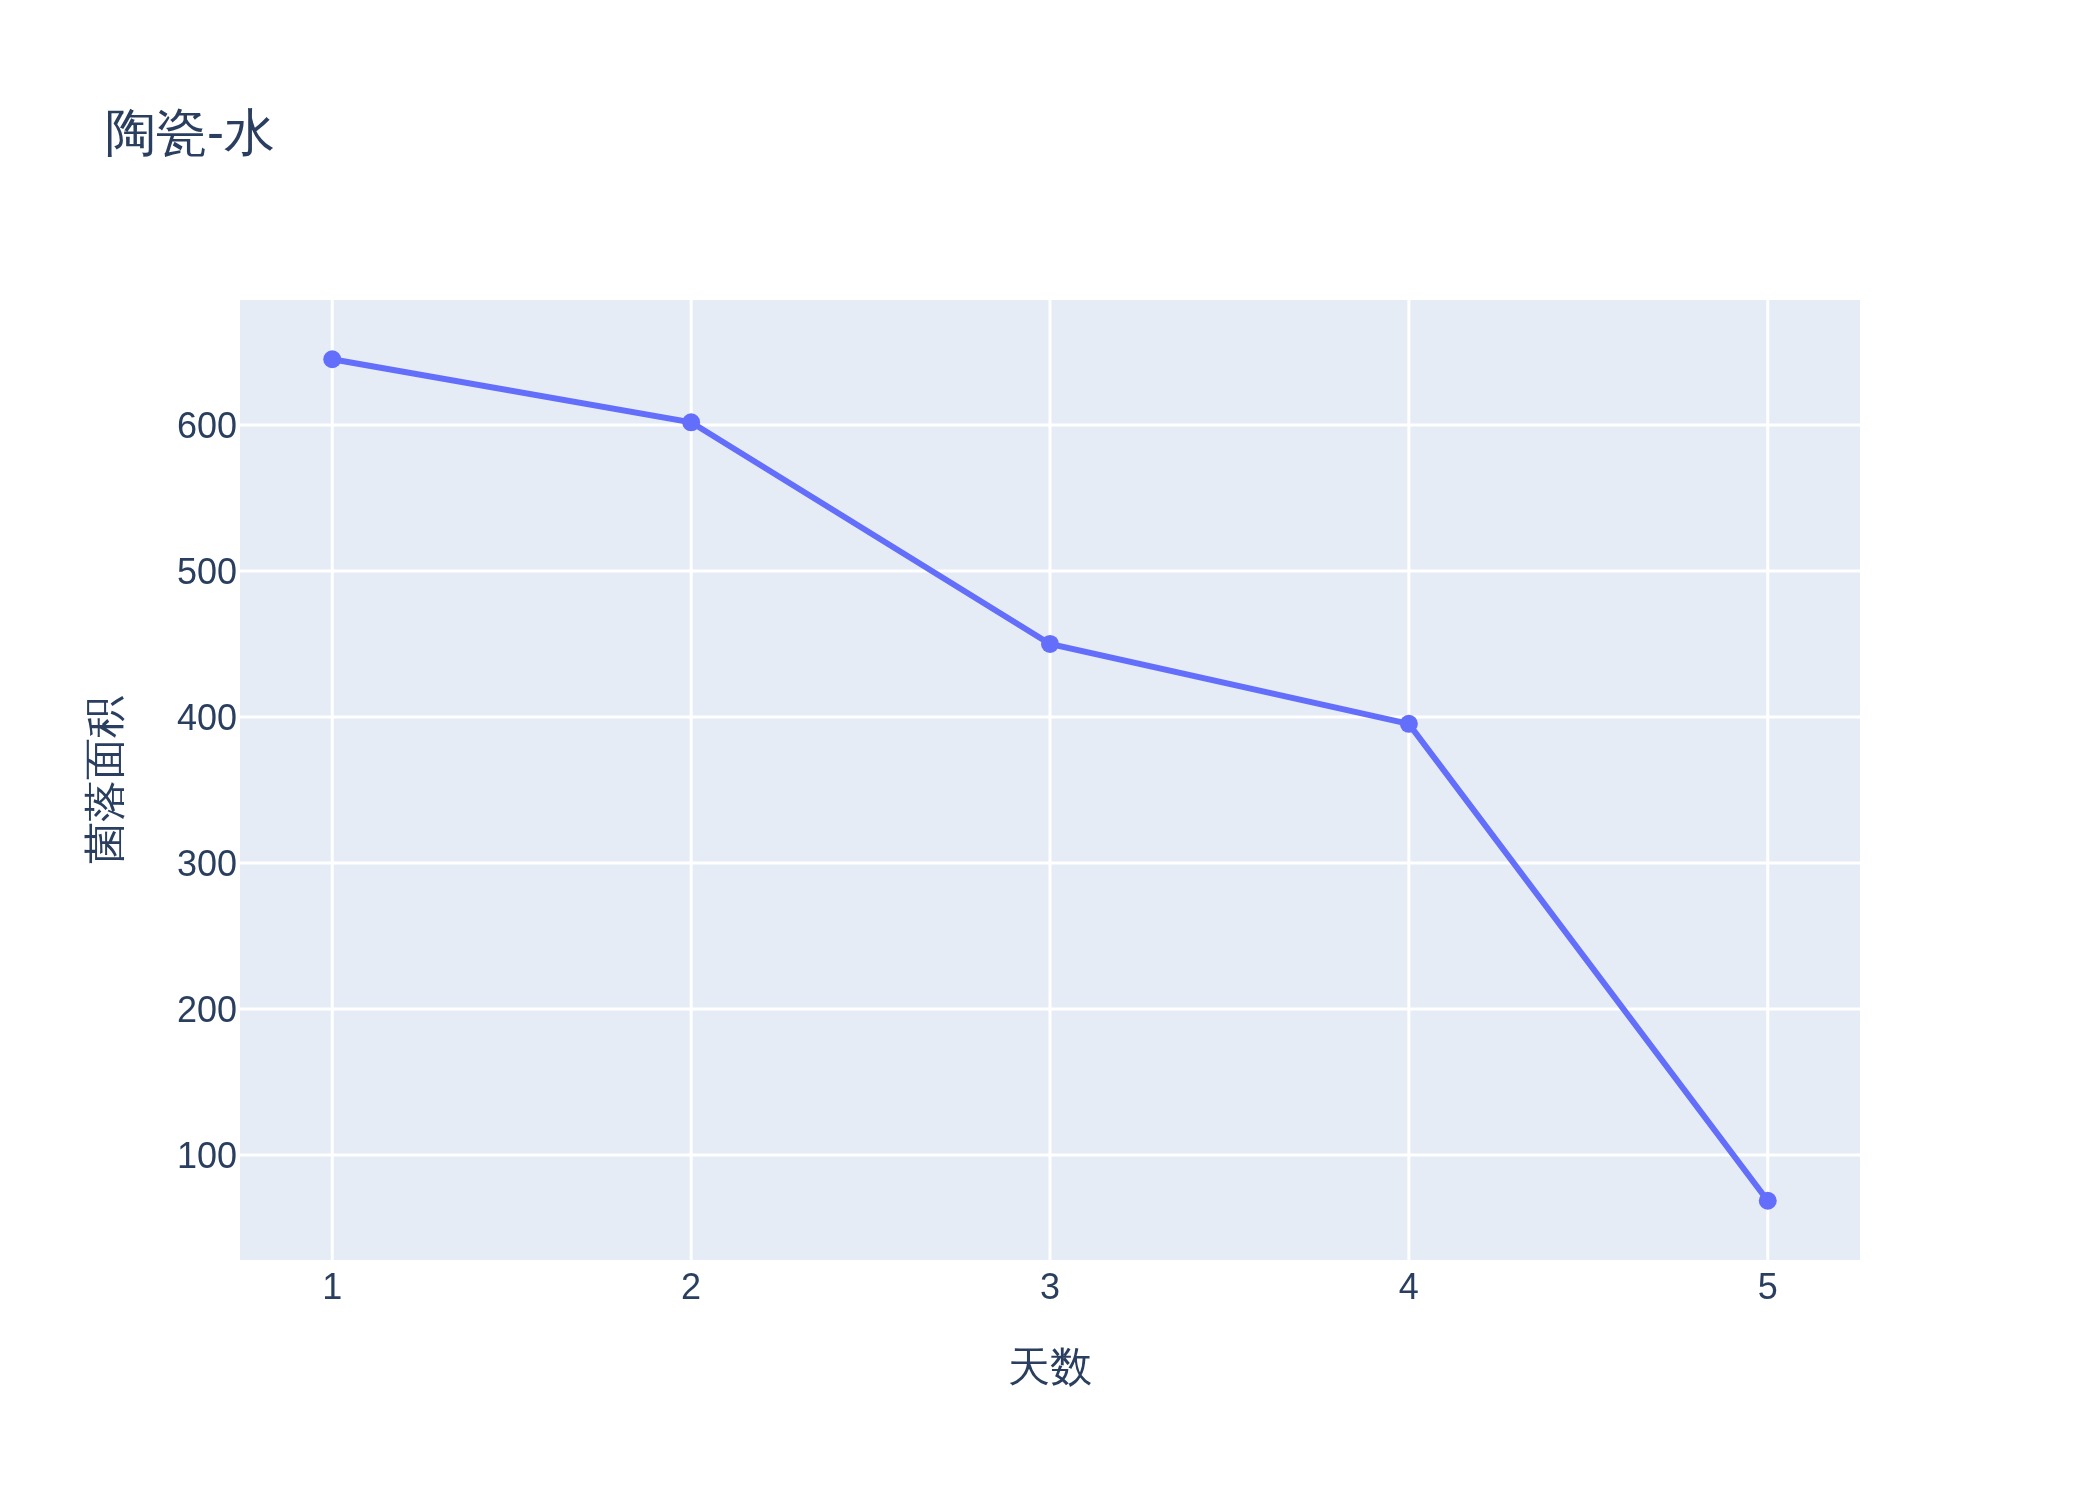
\includegraphics[width=\linewidth]{./plot/SingleMaterial/china/陶瓷-水_line.png}  % 替换为你的图片路径/文件名
        \caption{陶瓷-水}  % 子图1的标题
        \label{subfig:1}     % 子图1的引用标签(用于后文交叉引用)
    \end{subfigure}
    \hfill  % 子图间水平填充空白(均匀分布)
    % 子图2:与子图1宽度一致
    \begin{subfigure}[b]{0.31\textwidth}
        \centering
        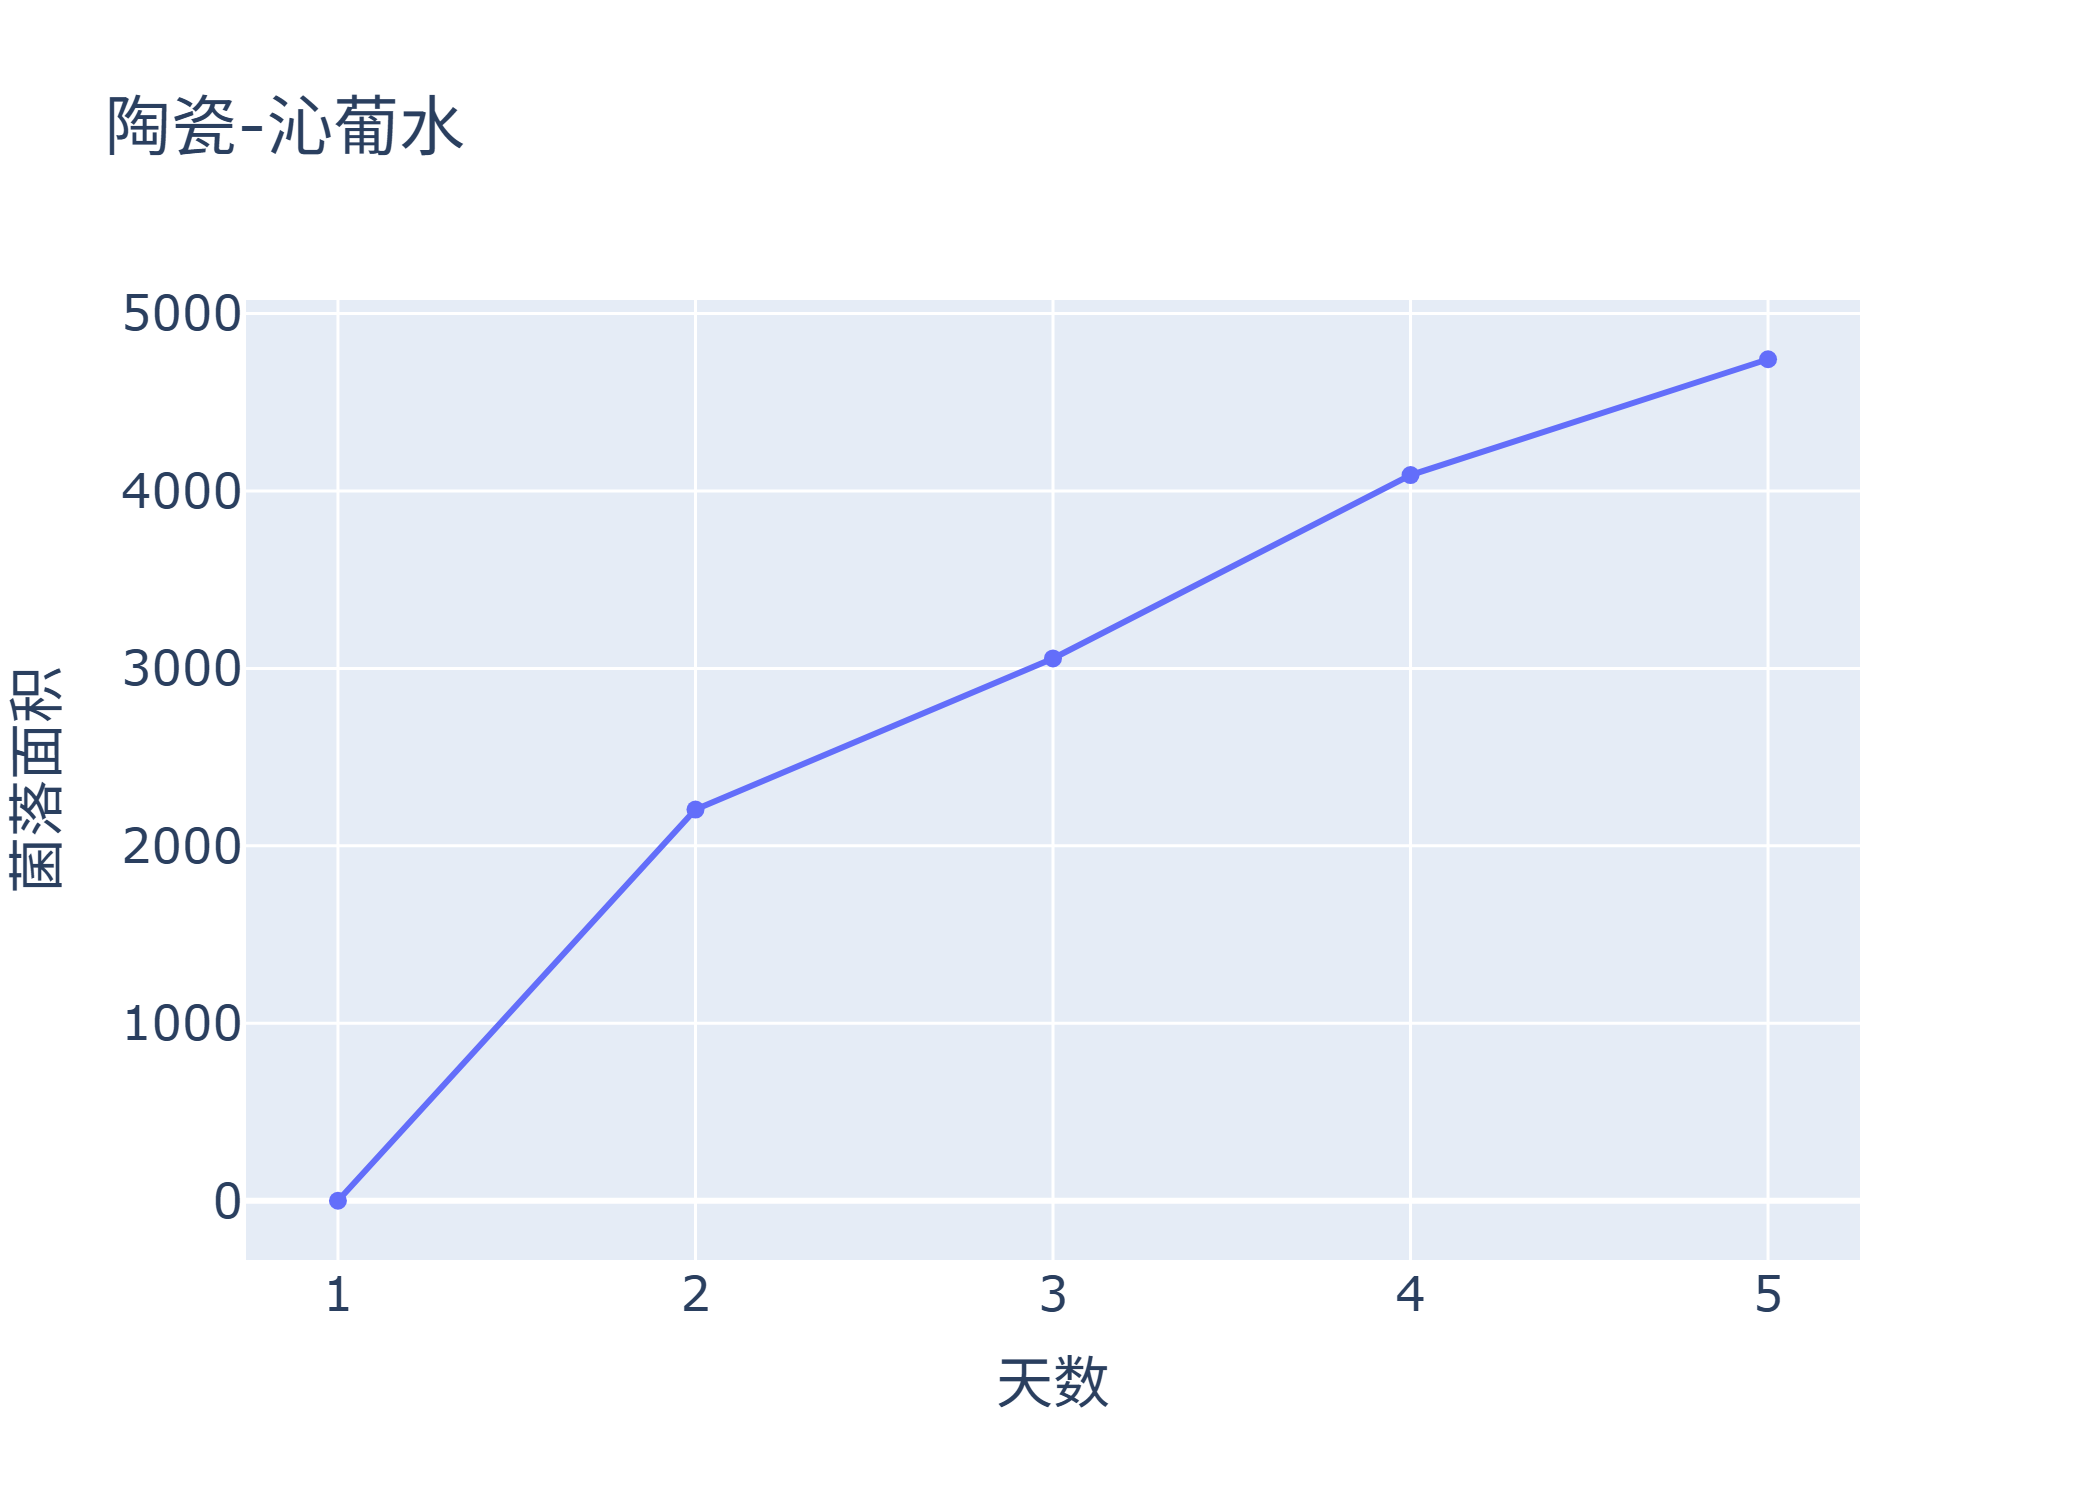
\includegraphics[width=\linewidth]{./plot/SingleMaterial/china/陶瓷-沁葡水_line.png}
        \caption{陶瓷-沁葡水}
        \label{subfig:2}
    \end{subfigure}
    \hfill  % 再次填充空白
    % 子图3:与前两个子图宽度一致
    \begin{subfigure}[b]{0.31\textwidth}
        \centering
        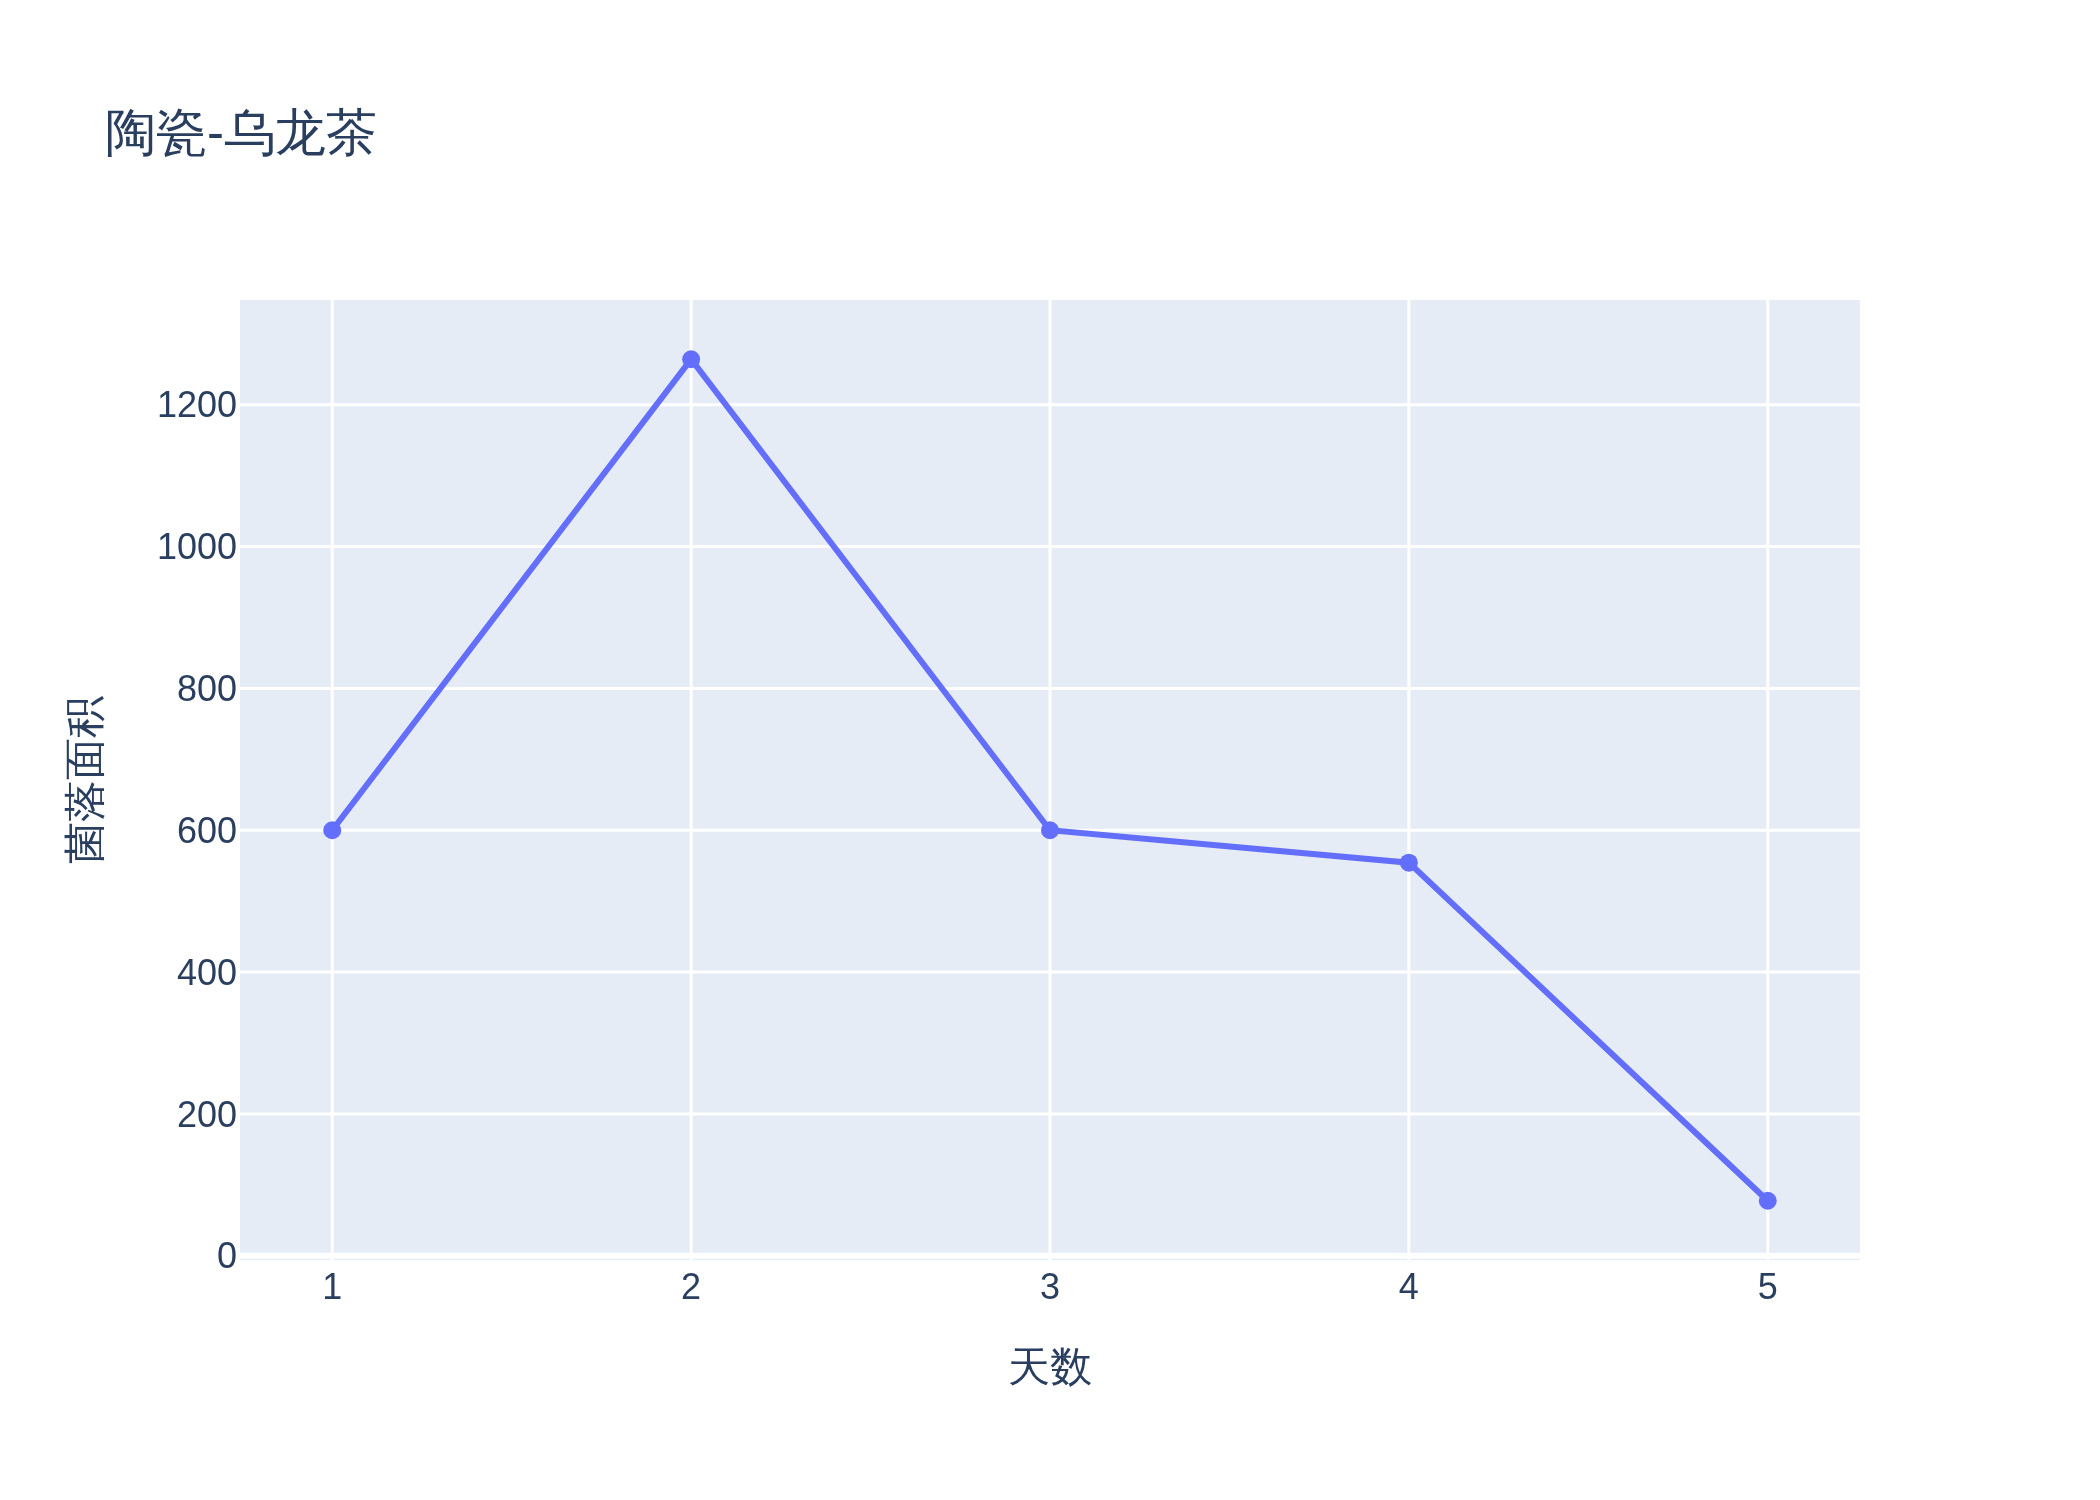
\includegraphics[width=\linewidth]{./plot/SingleMaterial/china/陶瓷-乌龙茶_line.png}
        \caption{陶瓷-乌龙茶}
        \label{subfig:3}
    \end{subfigure}
    % 整个三联图的总标题
    \caption{陶瓷片在3种溶液下的表面微生物情况}
    \label{fig:triple_horizontal}  % 整个图的引用标签
\end{figure}
\begin{itemize}
    \item 初期无菌水组带菌量较少,沁葡水平均带菌量最大,乌龙茶次之。
    \item 中期沁葡水组平均带菌量最大,乌龙茶组带菌量出现较大降低但平均带菌量仍高于水,而水组趋势不规律,平均带菌量最小。
    \item 后期沁葡水组有突降但平均带菌量仍最大,水组带菌量略有降低,但其平均带菌量高于乌龙茶,乌龙茶持续降低,带菌量最小。
\end{itemize}


\paragraph{控制承装液体相同,天数不同,可以得到:}
\begin{enumerate}
    \item 无菌水组:起始低,带菌量随天数不规律,有降低与突增,但大致上升。
    \item 沁葡水组:起始高,带菌量随天数上升,而在4天时有突降。
    \item 乌龙茶组:起始较高,带菌量随天数不规律下降。
\end{enumerate}
\subparagraph{总结}
对于在陶瓷杯中短期放置,依旧推荐灭菌过的水,长期放置时,乌龙茶所含菌量最少。而尽量不要存放含糖饮料。

\paragraph{原因分析}
\subparagraph{无菌水对微生物生长的影响}
实验所用水为无菌水,其本身不含微生物生长所需的营养物质,导致微生物初期生长速率缓慢,带菌量较少;同时,无菌水受环境影响较大,使得其中带菌量呈现出增长的态势。在铁片组的实验数据中,可以清楚得到这一点。而对于陶瓷片数据中初期与后期的异常减小,可能是实验培养误差所致。
\subparagraph{饮料营养成分对微生物生长的基础作用}
乌龙茶、沁葡水(含糖饮料)等饮品,均含有丰富的碳源及其他营养物质,这些成分能为微生物的代谢活动提供充足能量与物质基础,从理论层面而言,可显著促进微生物菌落的大量繁殖,这是此类富含营养成分的饮品相较于无菌水,在微生物生长支持能力上的共性特征。
\subparagraph{乌龙茶中抑菌物质对微生物生长的特殊调控}
尽管乌龙茶与沁葡水类似,可为微生物提供生长所需的碳源等营养,且其内部成分多样导致环境复杂度较高,但实际微生物生长情况并未呈现出与营养供给匹配的大量繁殖趋势。经资料查阅与分析可知,这一现象的核心原因在于乌龙茶中含有以多酚为代表的生物活性成分\cite{HXSJ202002001},该类成分具备显著的抑菌作用,能够抵消营养物质对微生物生长的促进效应,从而对微生物的生长繁殖形成特殊调控。

\subsection{不同材料,放置天数对同种饮料的影响}
\paragraph{无菌水}

根据数据,不难得出,在承装无菌水时,铁片与陶瓷的带菌总量差距并不大,但由于陶瓷片分析时采用增加偏置项的方法,而铁片采用拟合预算的方法。所以实际上,难以得出大小关系。
故对于水的承装,两种材料均可,并无影响。(待改)


\paragraph{沁葡水}
在承装沁葡水代表的含糖饮料中,陶瓷的带菌量远高于铁片。

故对于含糖饮料的承装,不锈钢杯子更好,能较有效的控制菌落生长,但仍然不适宜放置超过1天。

\paragraph{乌龙茶}
在承装乌龙茶时,大部分数据中铁片的带菌量依然小于陶瓷片,但差距并不大。

而对于茶类,不锈钢并非完全惰性,陶瓷杯则化学性质稳定。

故综合来看,我们更推荐使用陶瓷杯承装茶类,不锈钢杯子承装大部分无糖饮料。

\paragraph{原因分析}
\subparagraph{表面结构差异对微生物与营养物附着的影响}
相较于陶瓷片,不锈钢片经抛光处理后可形成极其光滑、无孔的表面,该表面特性显著减少了微观缺陷,使得微生物(如细菌、霉菌)及营养物(如糖分)难以嵌入或稳定附着。由于缺乏稳定的附着位点,微生物难以形成具有强附着力且难以清除的生物膜,这是两者在微生物附着层面的核心差异。
\subparagraph{表面光滑度对液体残留及糖分留存的影响}
不锈钢片的光滑表面会改变液体与材质的接触形态,在初始滴加液体时,液体更易以 “液滴” 状存在,而非像在陶瓷片表面那样铺展开并可能渗入材质内部。这种液滴形态使得后续转移或操作过程中,液体更易抖落,最终导致不锈钢片表面实际残留的糖分量通常略少于陶瓷片,而糖分作为微生物生长的重要营养来源,其残留量差异进一步影响了微生物的繁殖条件。
\subparagraph{附着位点数量对微生物生长繁殖状态的影响}
微生物的规模化生长繁殖往往依赖于在材质表面的稳定附着,而不锈钢片提供的有效附着点远少于陶瓷片。这一差异导致大部分细菌无法在不锈钢片表面牢固附着,只能悬浮于残留的液滴中,处于不稳定的生长状态,进而难以实现种群的大量增殖和规模化菌落的形成,最终表现为不锈钢片表面微生物生长受到明显抑制。

\subsection{分析与讨论}
\subsubsection{最佳承装液体}
综合数据看,乌龙茶所代表的无糖饮料中的茶类,因其特有的带菌量随天数逐步下降的数据,成为承装液体的不二之选。

\paragraph{原因分析}
\subparagraph{带菌量角度}
乌龙茶为代表的不含糖饮料。沁葡水本身为含糖饮料,可以给各种类细菌提供充足的水分以及糖分,作为前期繁殖的基础,因此初始数值大。但乌龙茶等无糖饮料中可能含有例如茶多酚等抑菌成分,这样使得细菌的繁殖受到抑制,因此无糖饮料中的细菌含量最低,具有一定的抑菌作用。而无菌水这一环境较为包容,也较为基础,只提供了水分,故初始带菌量小,但是也是可以被各种类细菌接受的适宜的生存环境,导致后续带菌量增幅较快。

\subsubsection{最佳承装容器}
陶瓷和铁片相比,铁片的抑菌性能更加优秀。然而在部分情况下,如承装茶类时,使用陶瓷杯,可能对承装液体更稳定。

\paragraph{原因分析}
\subparagraph{带菌量角度}
根据图像\ref{fig:GeneralLine}进行分析,我们发现无论是增长过程中还是下降过程中,虚线所代表的陶瓷始终位于实线所代表的铁片上方,即在相同天数,承装同种液体,铁片的带菌量均小于陶瓷,拥有更好的抑制菌落生长的能力。
\subparagraph{可能的风味影响角度}
在使用不锈钢杯子时,茶叶中的茶多酚、鞣酸等成分可能会与金属离子发生微弱的反应,或被金属表面催化氧化,导致茶汤颜色变深、变暗,甚至产生一种金属味。\cite{JSHJ201504002}。

使用陶瓷杯子,其坯体和表面的釉(指无彩绘的透明釉)经过高温烧制后,形成了一种非常稳定、致密的玻璃态物质,使得它不会与茶叶中的茶多酚、鞣酸、咖啡中的酸性物质等发生化学反应。 

\section{结论与创新点}
\subsection{结论}
综上所述,我们根据实验数据与严谨的处理、分析过程后得出如下结论:
\begin{itemize}
    \item 对于水的承装,两种材料均可,并无影响。
    \item 对于含糖饮料的承装,更推荐表面光滑的不锈钢杯子,但仍然不适宜放置过久。
    \item 对于茶类饮品的承装,推荐使用陶瓷制品。
\end{itemize}

\subsection{创新点}
在我们的研究中,我们实现了如下创新:
\begin{itemize}
    \item 为了使数据合理化,引入了计算机科学领域常用的“偏置”方法,保证各实验组的初始条件尽可能一致
    \item 我们在实验过程中并未采取具体的实际的水杯进行实验,而是使用了材质类似的金属片、陶瓷片,以此来尽量减少杯子形状深度大小等因素对于实验结果的影响。
\end{itemize}

\section{问题与反思}\label{sec:problem}
\subsection{现有问题}
在本次研究中,出现了如下问题,可能会导致实验数据偏差从而得出错误的结论,包括但不限于:
\begin{enumerate}
    \item 在本次实验中,我们没有很好地控制变量,在进行实验时,部分材料的1,2,3天与4,5天的样本分开进行了采集,因此难以排除气候以及其他两次实验中由于操作或其他原因导致的误差。
    \item 本次实验样本较少,部分样品由于实验过程中的原因产生了损耗,这会导致实验结果可能不具备可复现性,以及实验的结果可能并不具备说服力。另外,本次实验的材料种类过少,原定为4种材料进行交叉比对,然而由于时间有限,导致实验流程被大大压缩,所以只实验了三种材料,种类过少可能不能精确找到最佳抑菌材料。
\end{enumerate}

\subsection{反思与改进方案}
针对如上问题\ref{sec:problem},我们提出了如下解决方案:
%IMPORTANT!:这是有序列表,有编号的,每个点应当与问题一一匹配
\begin{enumerate}
    \item 对于问题1,应该尽量合理地安排实验流程,将同种材料的实验放在尽量相近并且同时的时间进行,并且精确化采样时间和培养时长,以确保实验结果的准确性。
    \item 对于问题2,可以对于同一天数同一材料同一饮料的实验样品多次重复并留出一定的冗余,并且丰富化材料种类,从真正市面上的保温杯以及咖啡杯上进行采样,确保实验的真实可靠。
\end{enumerate}

\subsection{未来展望}
针对以上问题及解决方案,我们希望未来能够进一步跟进研究,得出更多可靠、更完备的结论,包括但不限于:
\begin{itemize}
    \item 希望基于以上更为丰富完善的实验流程得到市面上同种饮料盛装于各种材质制作而成的水杯中,随着时间天数变化的菌落面积和数量曲线,以此来选出具有最佳抑菌效果的水杯材料。
    \item 针对不同饮料营养成分以及不同材质的水杯得到理论的必要清洗频率以及最佳清洗频率,以避免不频繁的清洗导致菌落数量大幅增长或者是过于频繁的清洗。
\end{itemize}

\section{收获}
本研究在认知、科研实践、应用成果三方面实现递进式收获。认知上,突破 “不喝隔夜水” 经验局限,明确饮料残留营养物质和容器材质表面特性是卫生隐患核心,结合美国数据与实验现象,发现含糖饮料菌落数远高于无菌水,不锈钢因表面光滑抑制细菌增殖,陶瓷易形成稳定菌落。

实践中,掌握高压蒸汽灭菌等关键技能,遵循科研原则,通过设置对照、时间梯度和材质变量,分析 “材料 - 饮料 - 时间” 对细菌增殖的影响,强化完整科研能力。

应用上,形成实用价值:生活中明确不同材质水杯适配饮品及清洗要求;产业上为水杯制造提供方向,相关模型还可为食品包装等领域卫生研究提供参考 。

% 致谢页通常单独成页,不编号
\clearpage
\thispagestyle{empty} 
\section{致谢} % 带星号的section表示不编号

本论文的顺利完成,离不开众多师长、同学和亲友的鼎力支持与帮助。在此,我们谨向他们致以最诚挚的谢意。

首先,我要衷心感谢我的导师张阳老师。从论文的选题、框架设计到具体内容的修改完善,张老师都倾注了大量心血,给予了我悉心的指导和无私的帮助。张老师严谨的治学态度、深厚的学术素养和诲人不倦的师者风范,令我受益匪浅,并将激励我在未来的学习和工作中不断前进。

感谢在学习期间所有为我授业解惑的老师们,他们的精彩课程为我打下了坚实的专业基础,拓宽了我的学术视野。

感谢实验室的各位同门和同学们,在论文写作过程中,我们相互探讨、共同进步,你们的陪伴和支持让我在科研道路上不再孤单。

感谢参与本论文评审和提出宝贵意见的各位专家学者,他们的真知灼见为论文的完善提供了重要指导。

最后,我们要向我们的家人表示最深切的感谢。你们的理解、支持和鼓励是我能够安心完成学业和论文写作的坚强后盾。

由于我们学识水平有限,论文中难免存在疏漏和不足之处,恳请各位老师和专家批评指正。\newpage

\clearpage
\thispagestyle{empty} 
\section{附录A:相关图表}
\subsection{总体图表}
\begin{figure}[H]  % [H] 表示强制在此处插入(不浮动),也可用 htbp 等浮动选项
    \centering  % 图片居中显示
    % width=\textwidth 让图片宽度等于页面宽度(自动适应)
    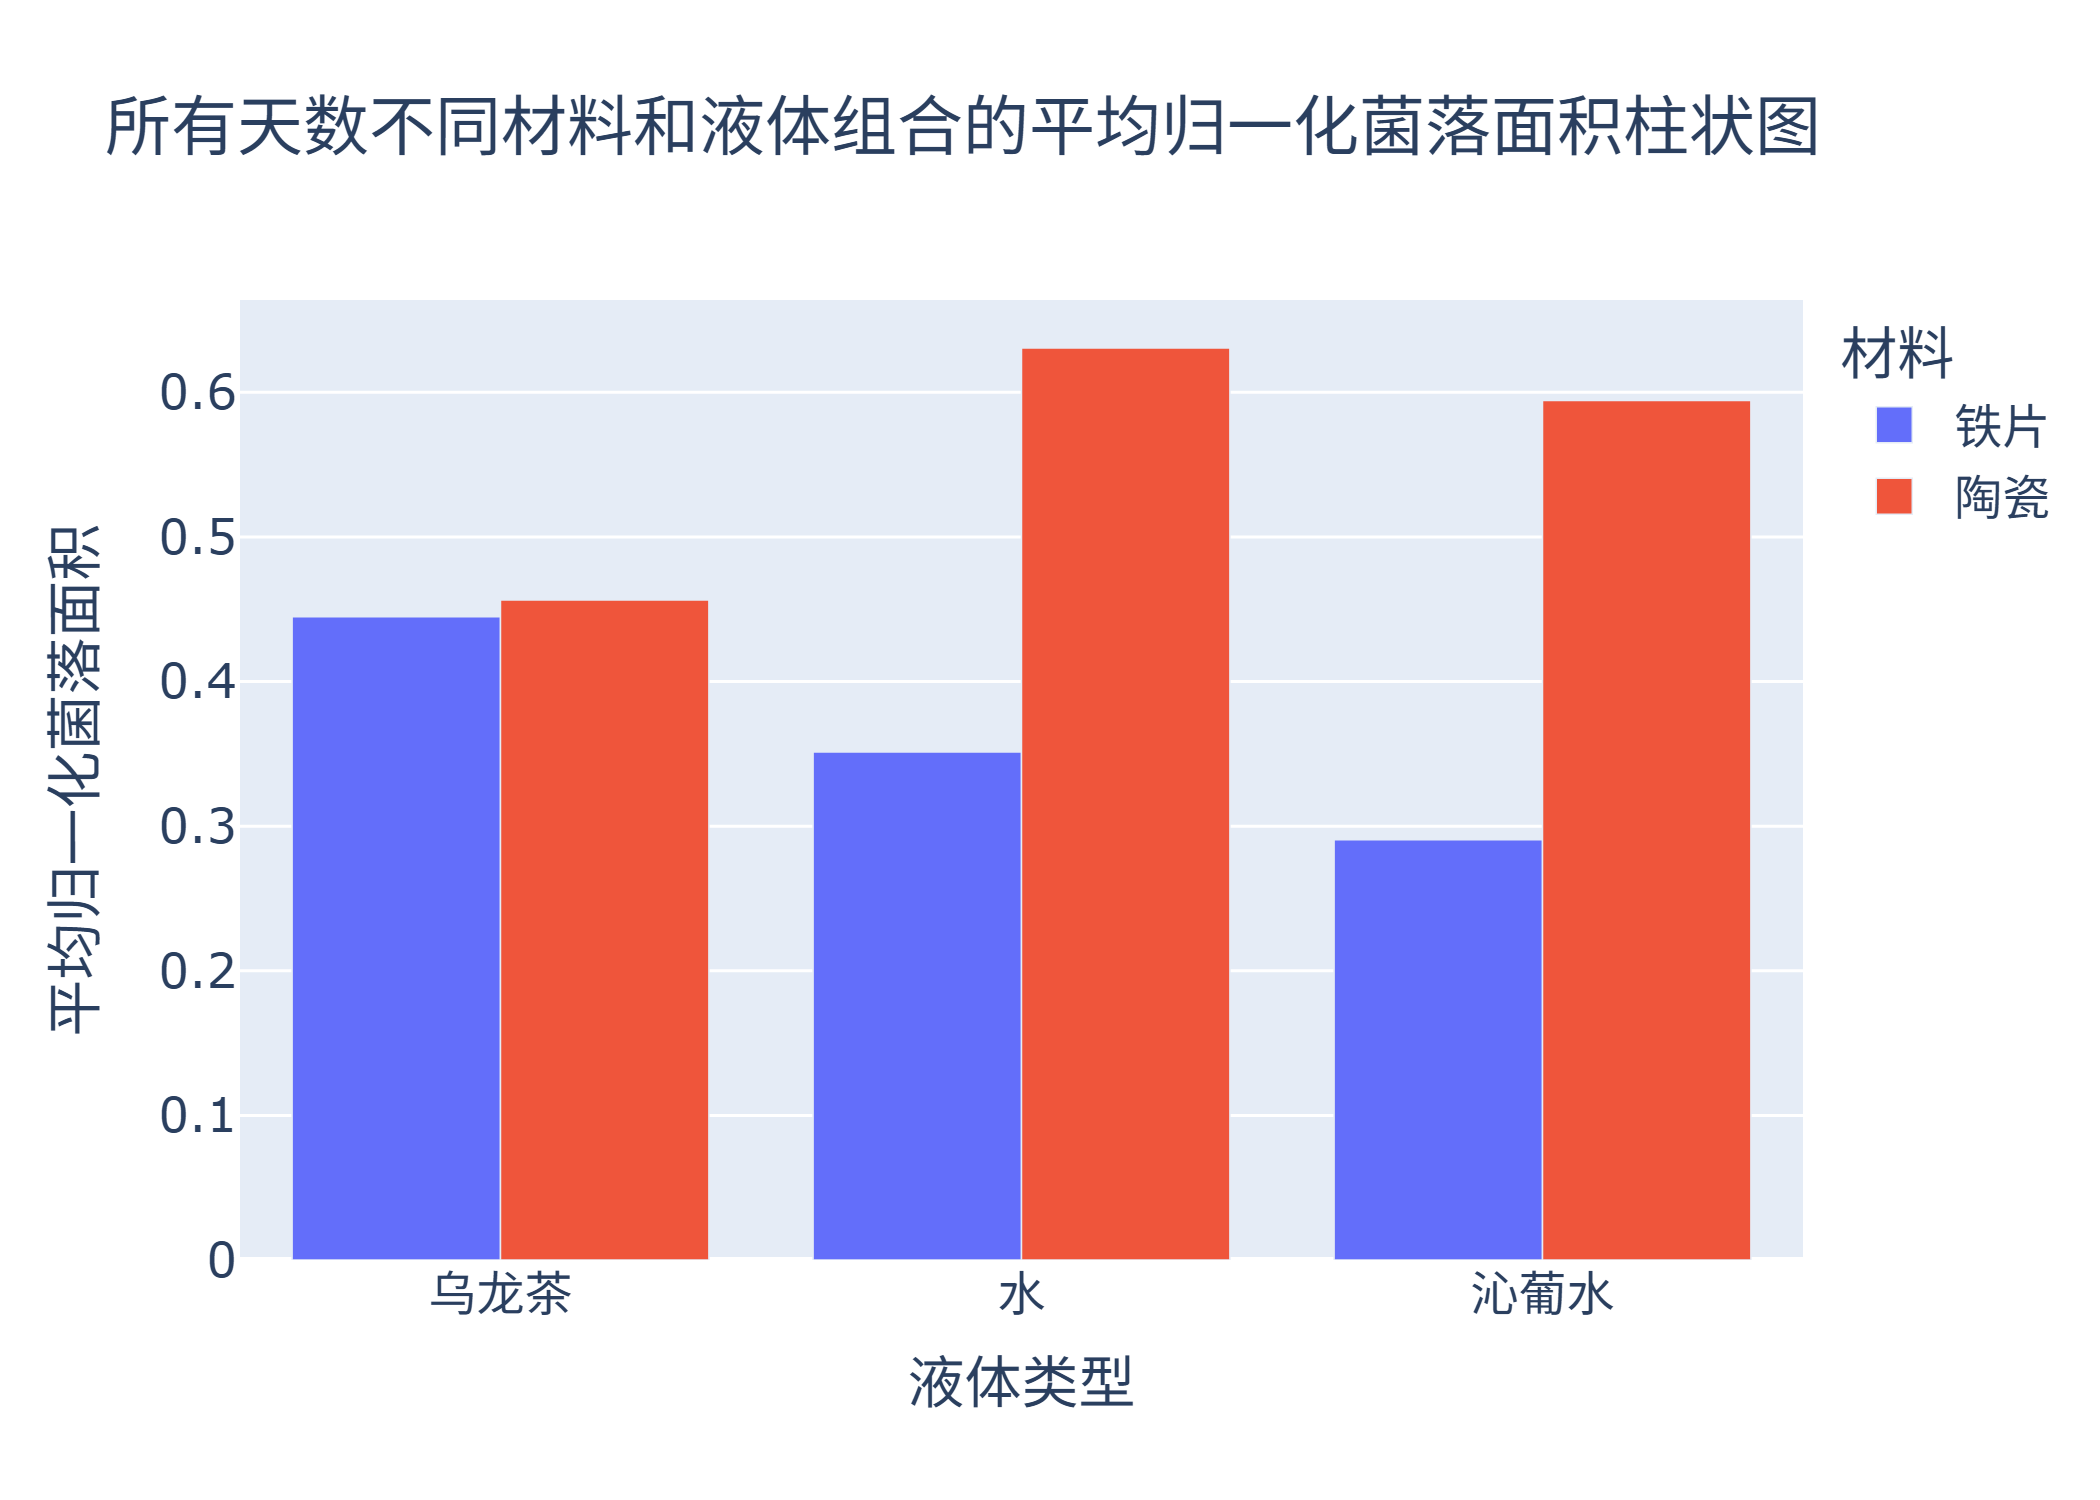
\includegraphics[width=\textwidth]{./plot/General/bar_normalized_overall.png}  % 替换为你的图片路径/文件名
    \caption{总体柱状图}  % 图片标题
    \label{fig:GeneralBar}  % 标签,用于后文引用
\end{figure}

\begin{figure}[H]  % [H] 表示强制在此处插入(不浮动),也可用 htbp 等浮动选项
    \centering  % 图片居中显示
    % width=\textwidth 让图片宽度等于页面宽度(自动适应)
    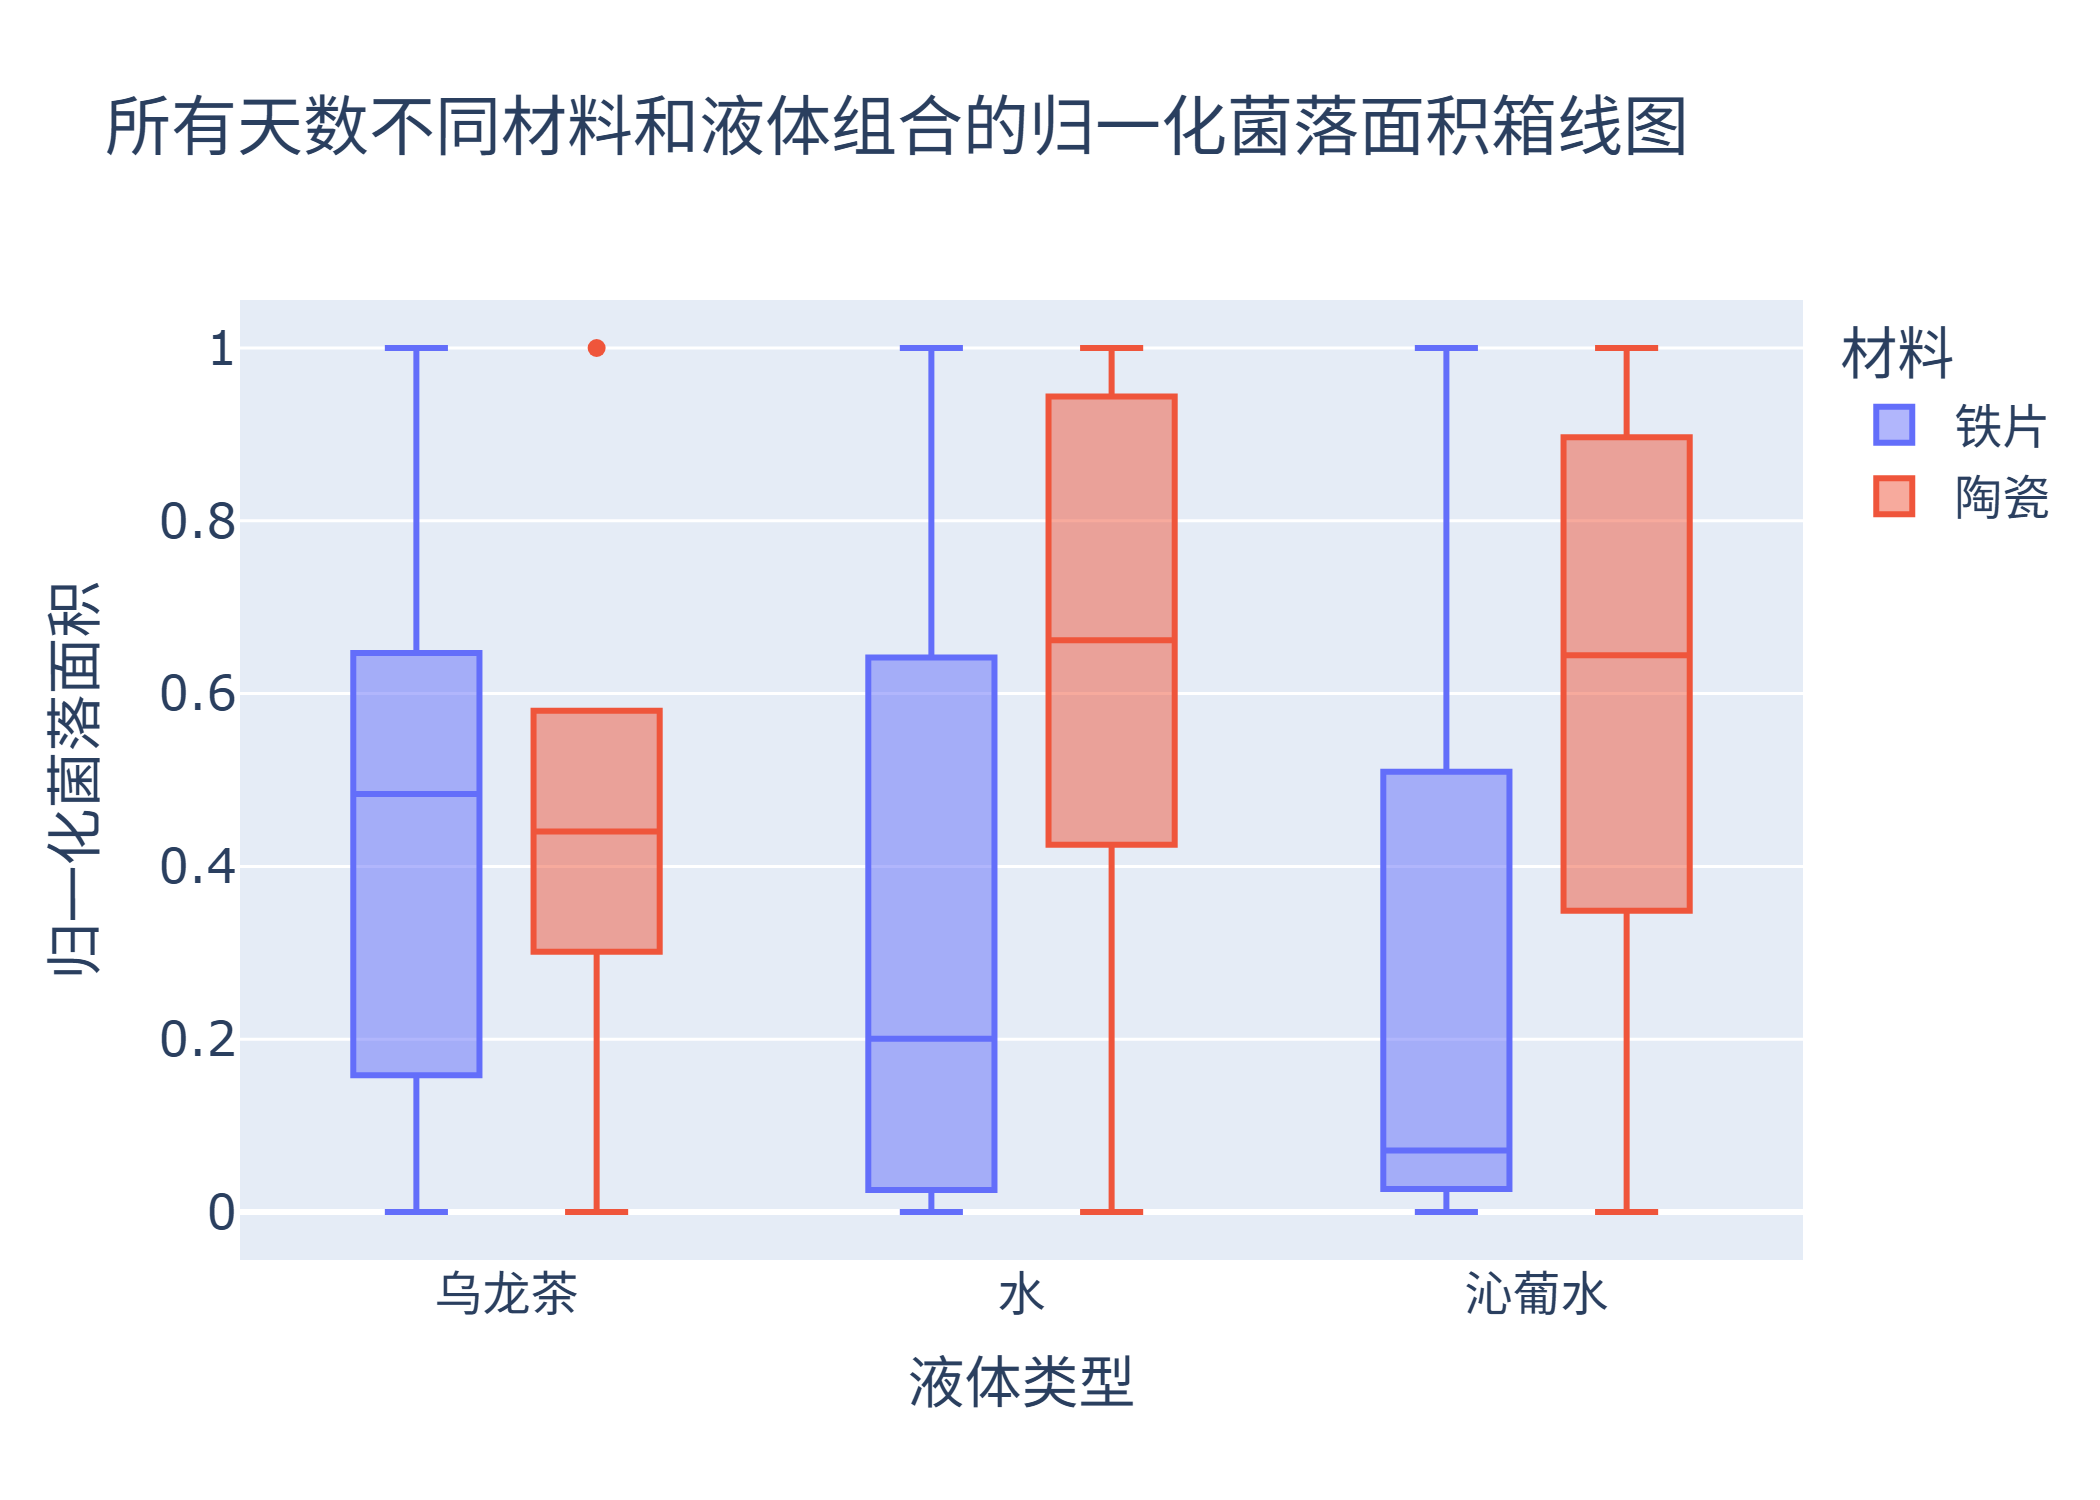
\includegraphics[width=\textwidth]{./plot/General/boxplot_normalized_overall.png}  % 替换为你的图片路径/文件名
    \caption{总体箱线图}  % 图片标题
    \label{fig:GeneralBox}  % 标签,用于后文引用
\end{figure}

\begin{figure}[H]  % [H] 表示强制在此处插入(不浮动),也可用 htbp 等浮动选项
    \centering  % 图片居中显示
    % width=\textwidth 让图片宽度等于页面宽度(自动适应)
    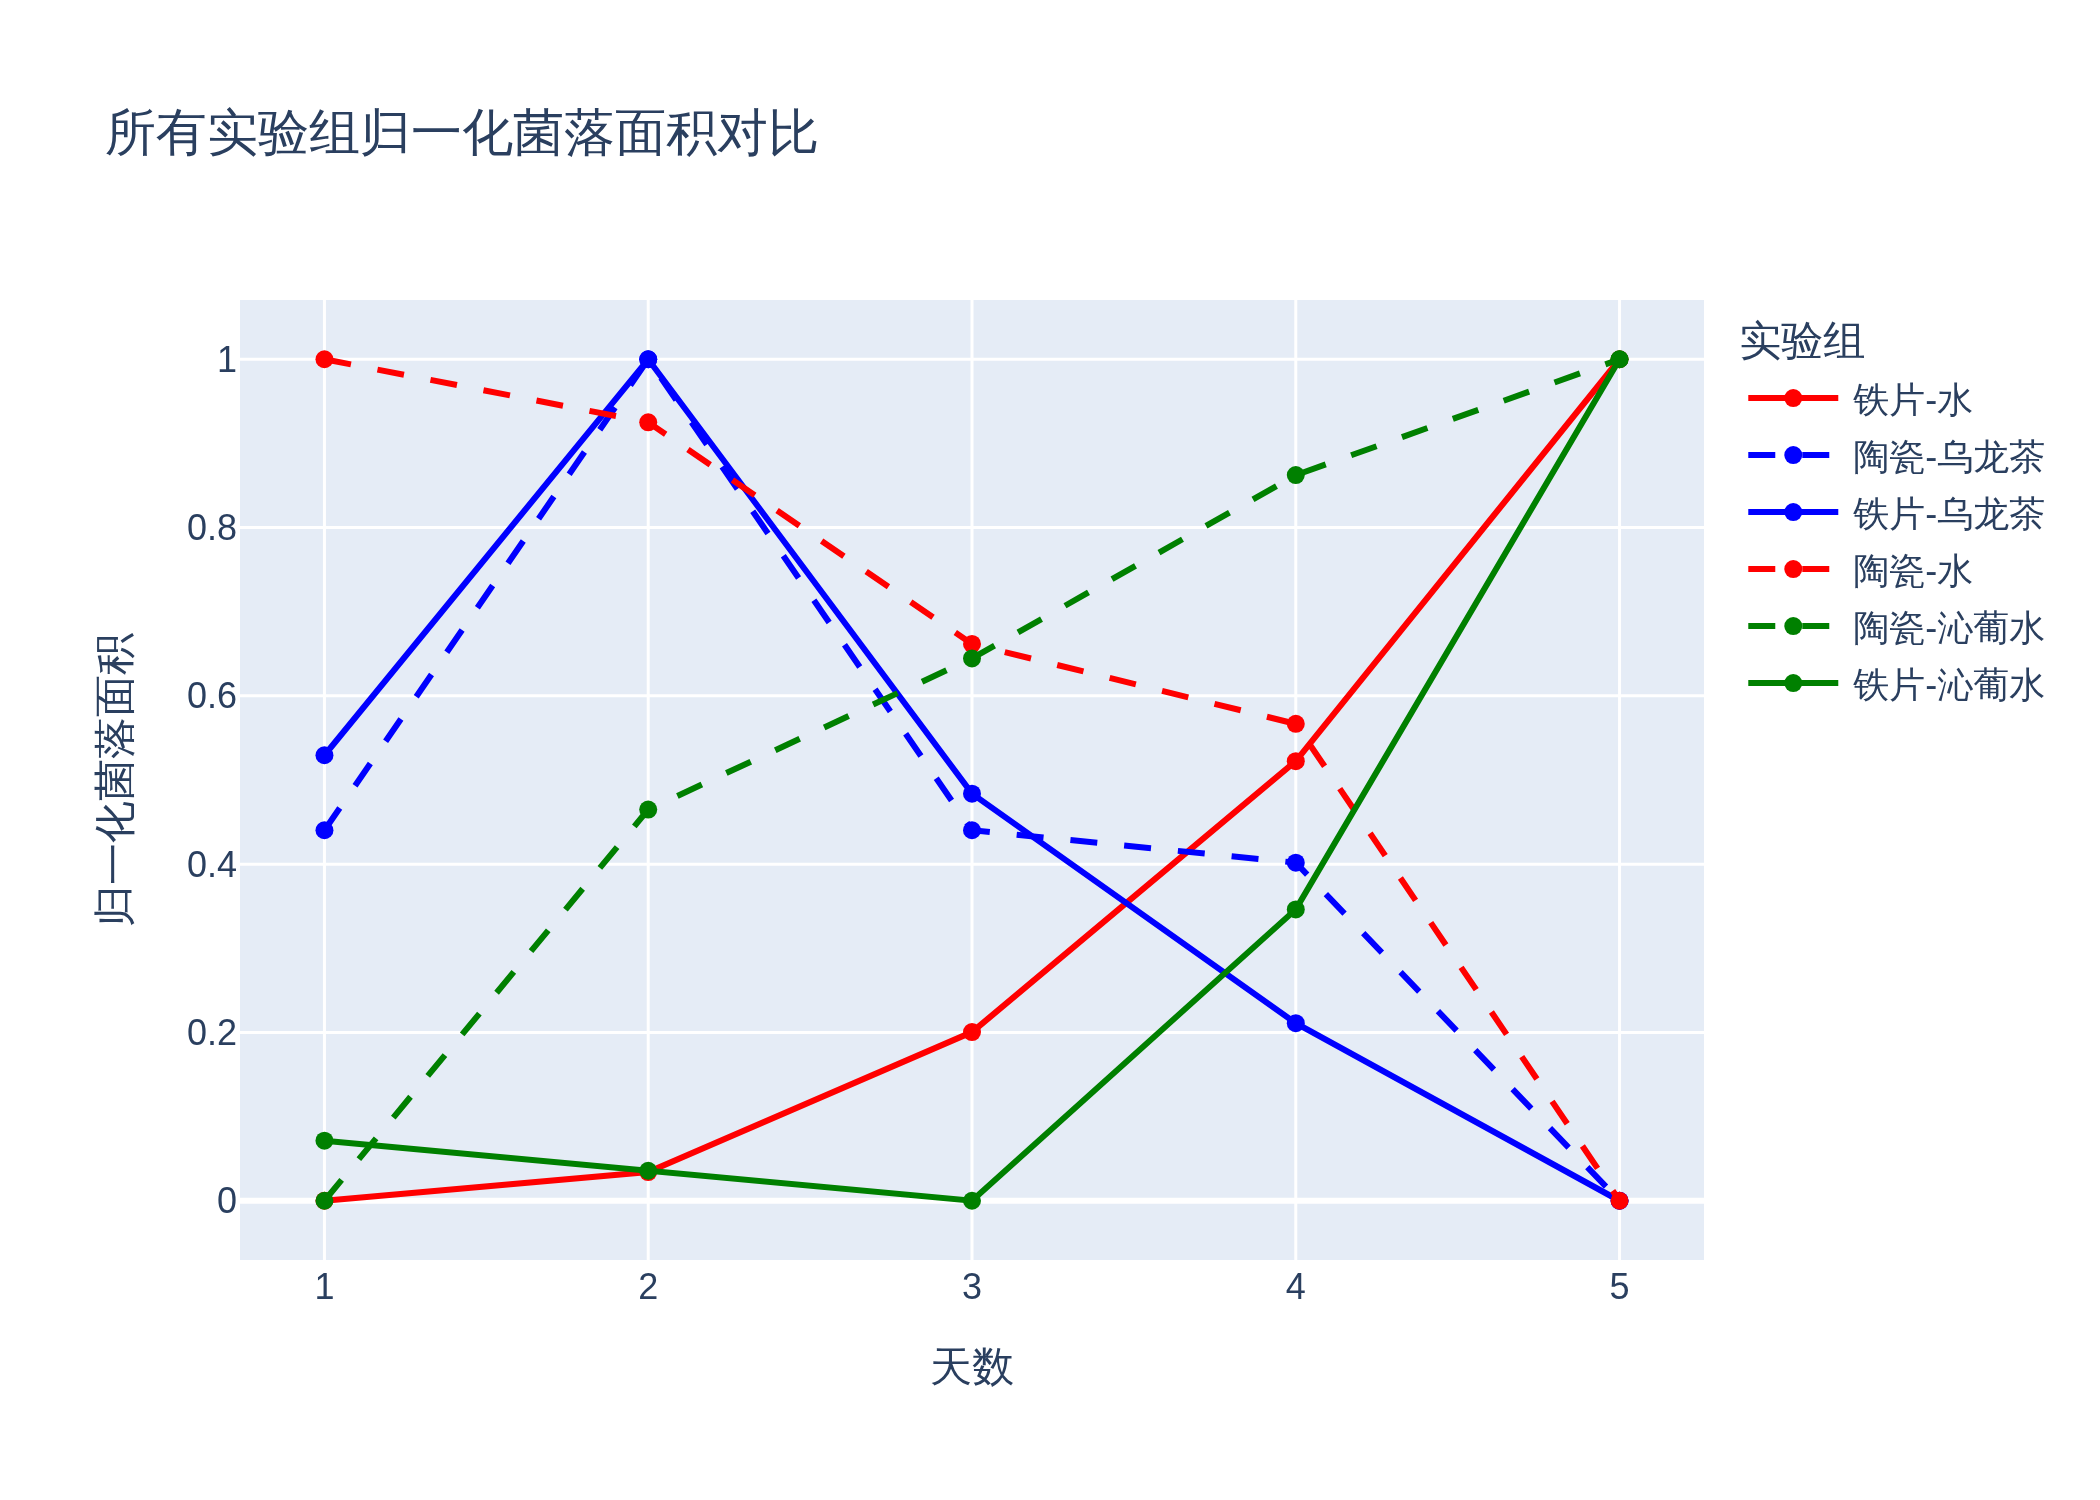
\includegraphics[width=\textwidth]{./plot/General/combined_normalized_line.png}  % 替换为你的图片路径/文件名
    \caption{总体折线图}  % 图片标题
    \label{fig:GeneralLine}  % 标签,用于后文引用
\end{figure}

\begin{figure}[H]  % [H] 表示强制在此处插入(不浮动),也可用 htbp 等浮动选项
    \centering  % 图片居中显示
    % width=\textwidth 让图片宽度等于页面宽度(自动适应)
    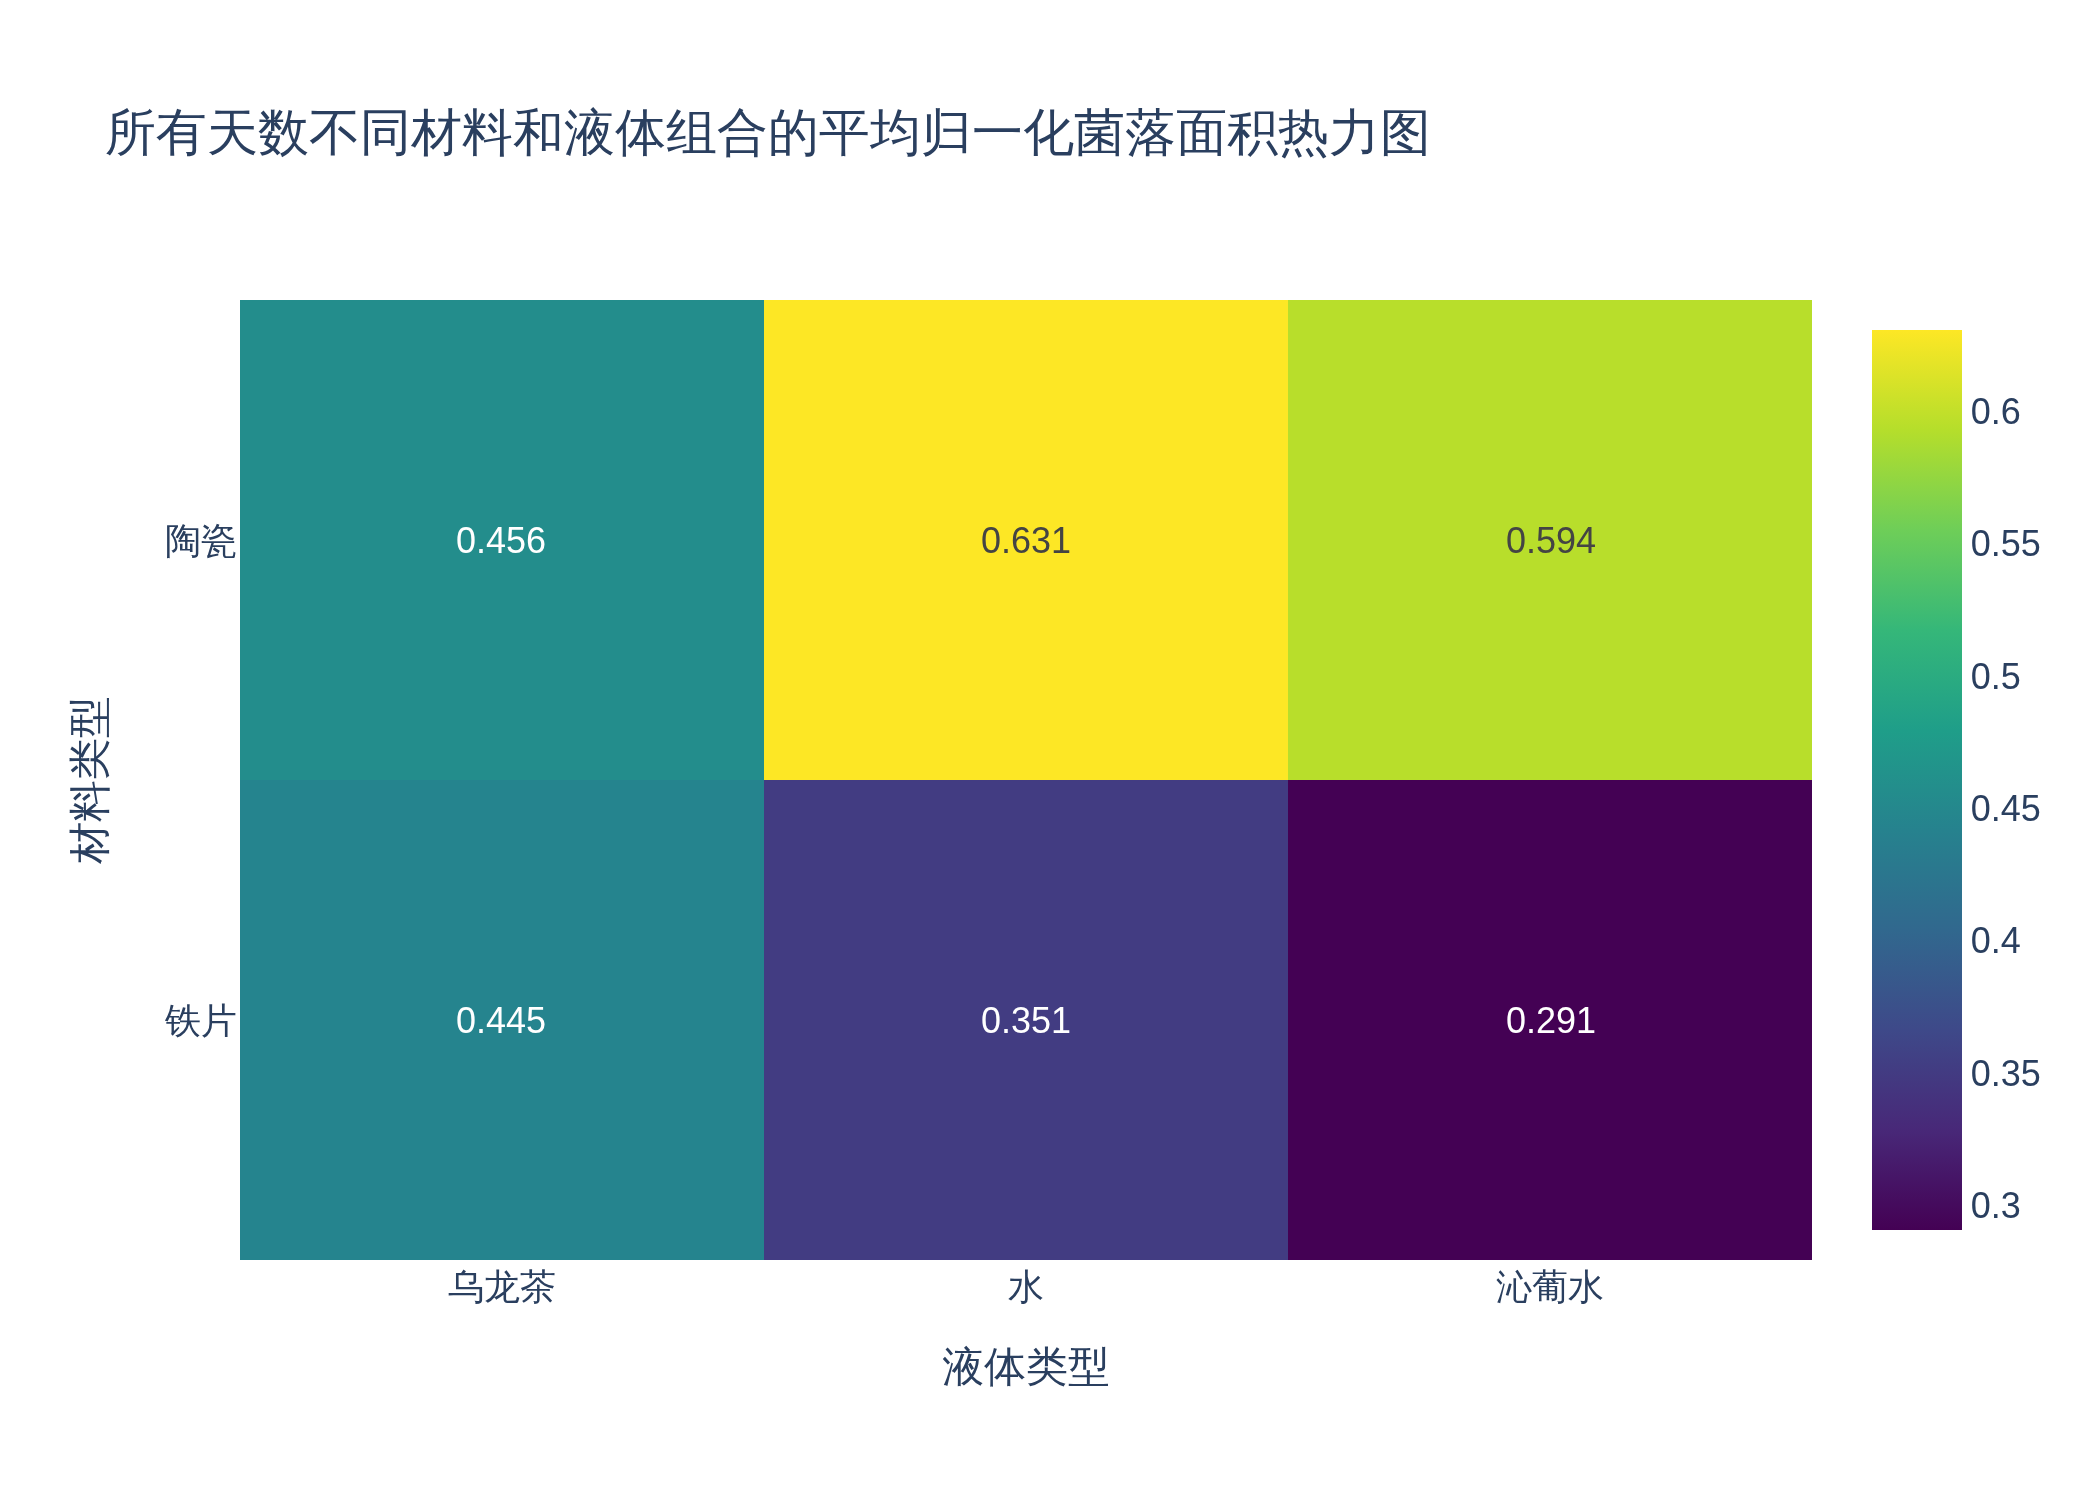
\includegraphics[width=\textwidth]{./plot/General/heatmap_normalized_overall.png}  % 替换为你的图片路径/文件名
    \caption{总体热力图}  % 图片标题
    \label{fig:GeneralHeat}  % 标签,用于后文引用
\end{figure}

\begin{figure}[H]  % [H] 表示强制在此处插入(不浮动),也可用 htbp 等浮动选项
    \centering  % 图片居中显示
    % width=\textwidth 让图片宽度等于页面宽度(自动适应)
    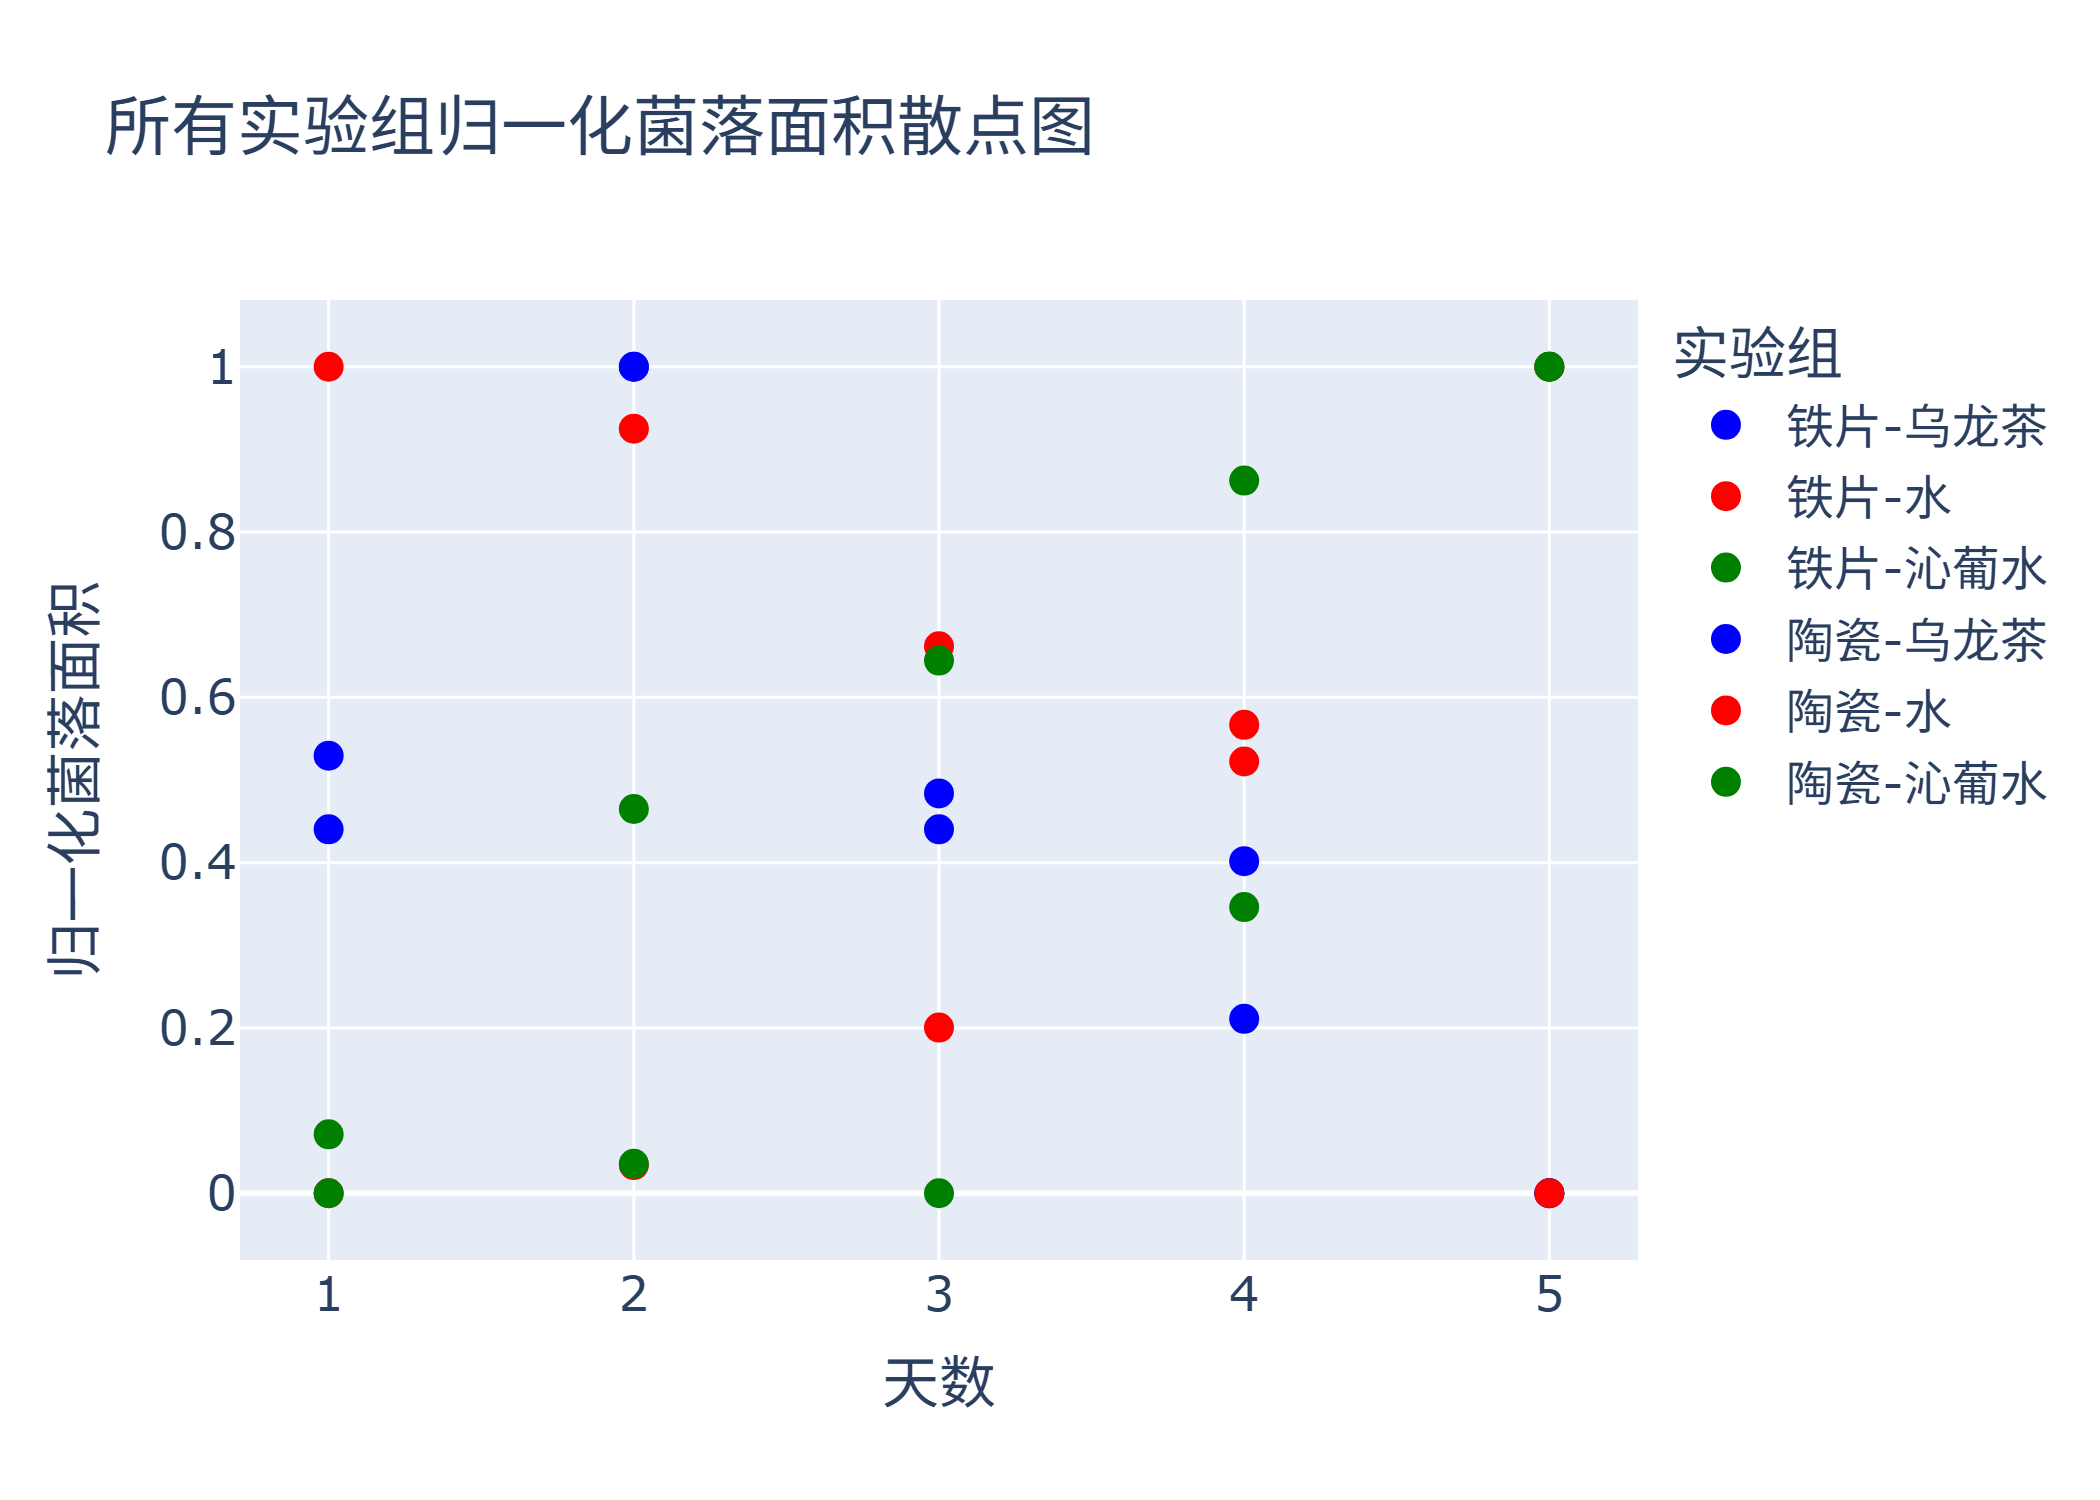
\includegraphics[width=\textwidth]{./plot/General/scatter_normalized_overall.png}  % 替换为你的图片路径/文件名
    \caption{总体散点图}  % 图片标题
    \label{fig:GeneralScatter}  % 标签,用于后文引用
\end{figure}
\subsection{天数相同,材料、溶液不同的归一化柱状图}
\begin{figure}[H]  % [H] 表示强制在此处插入(不浮动),也可用 htbp 等浮动选项
    \centering  % 图片居中显示
    % width=\textwidth 让图片宽度等于页面宽度(自动适应)
    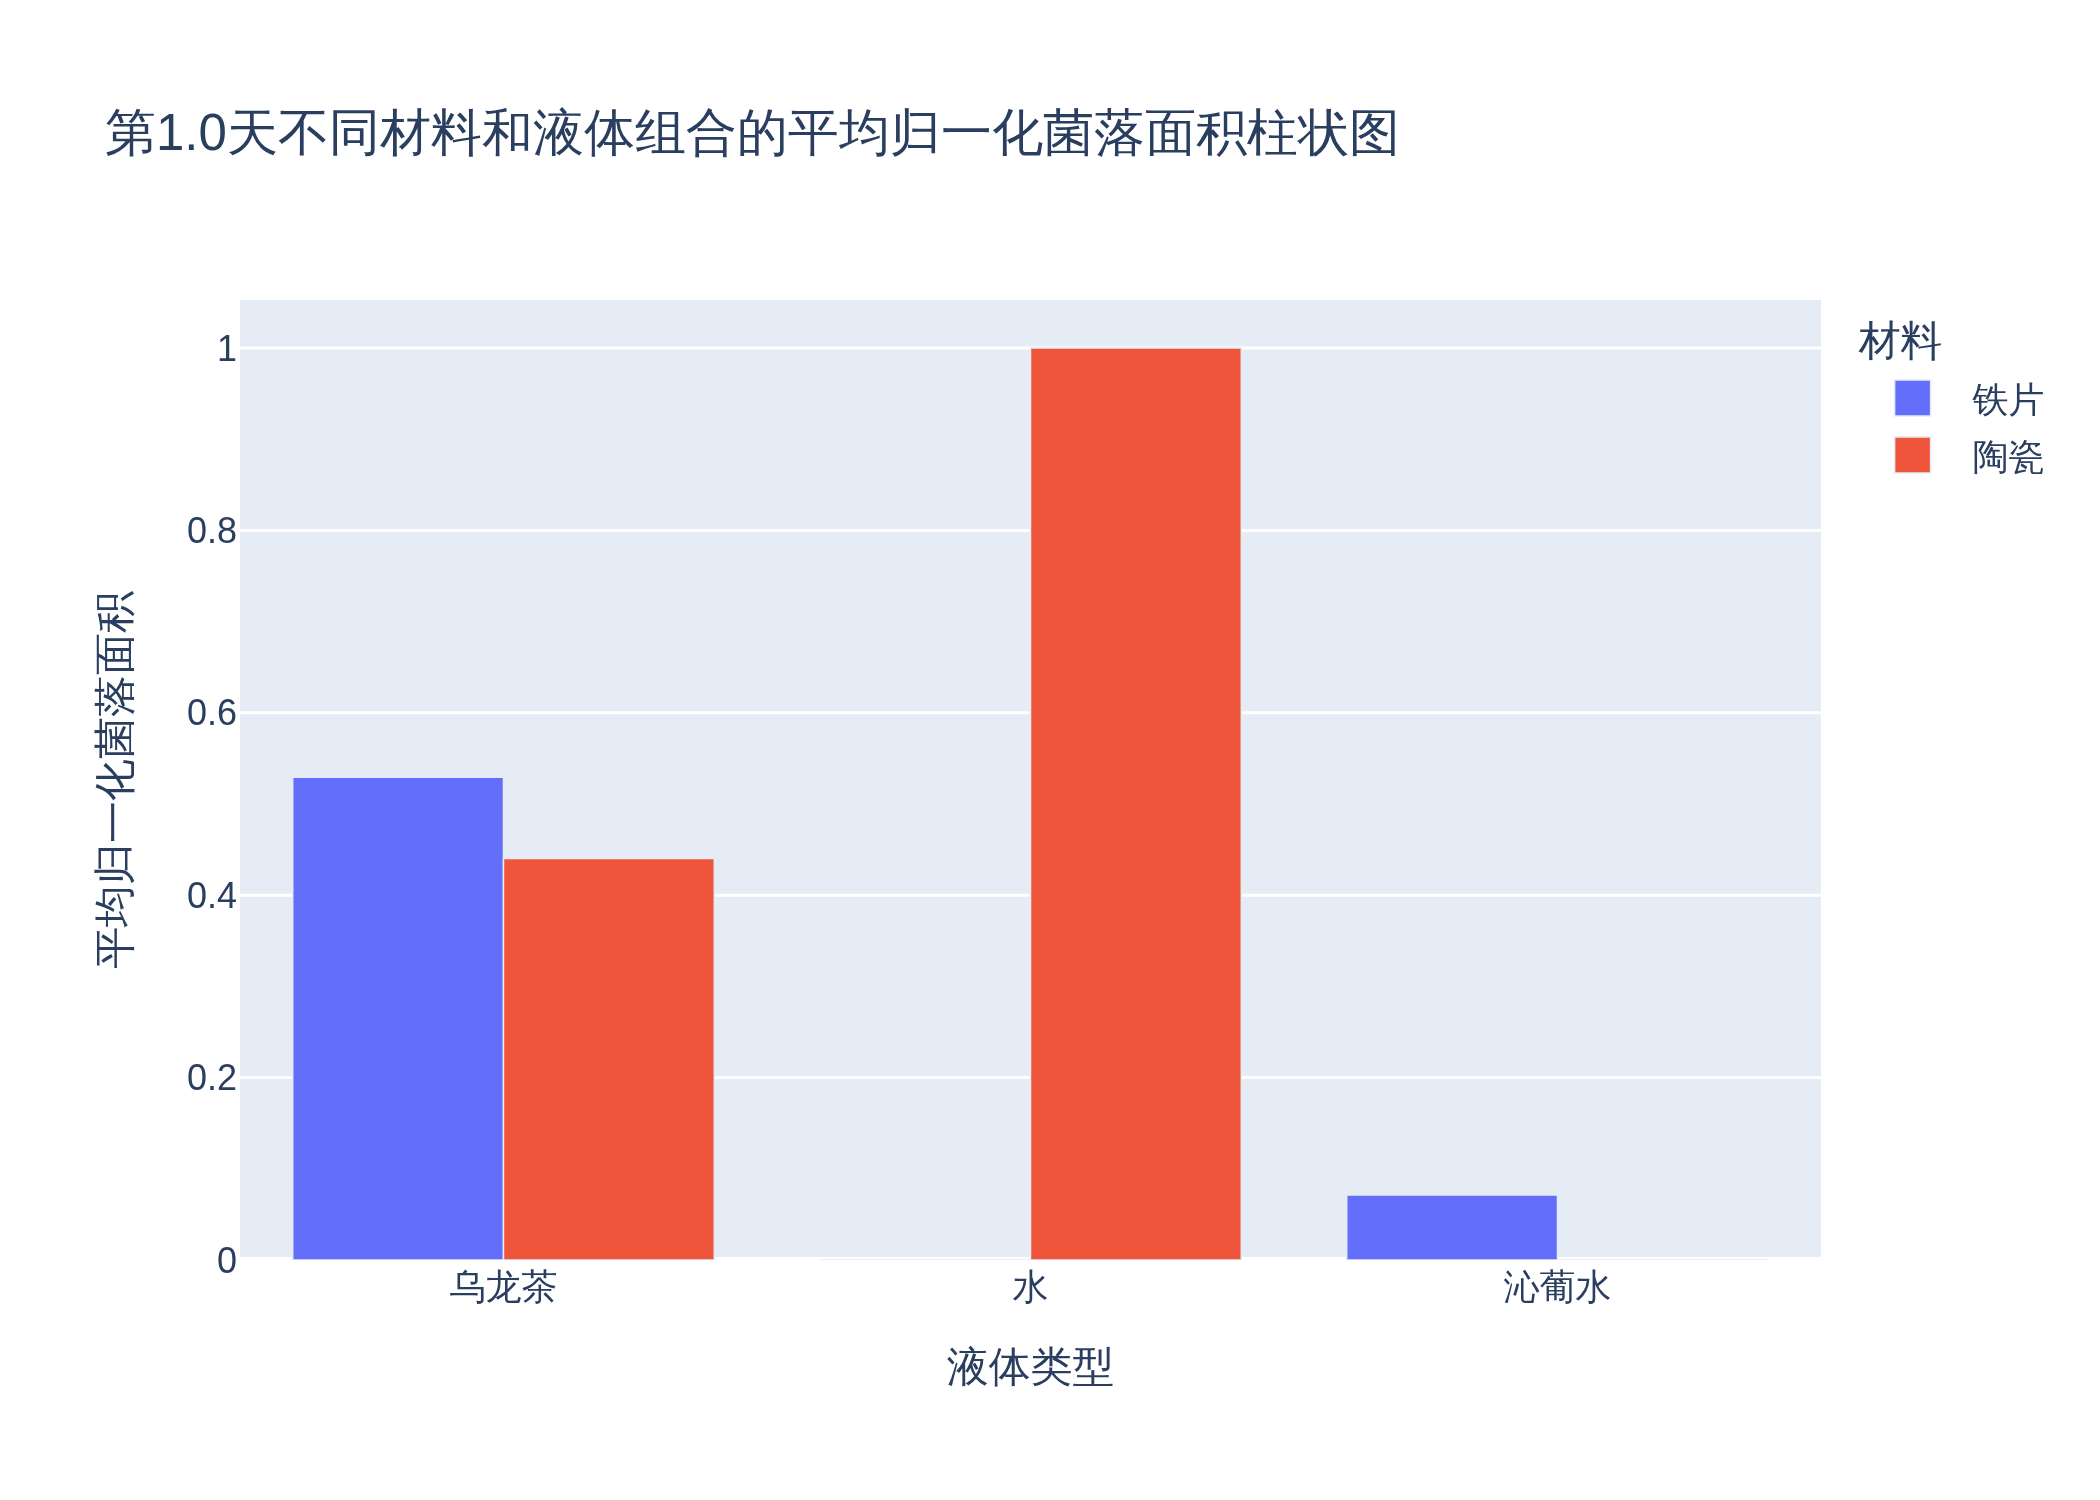
\includegraphics[width=\textwidth]{./plot/SingleDay/bar_normalized_day1.0.png}  % 替换为你的图片路径/文件名
    \caption{第一天}  % 图片标题
    \label{fig:SingleDayBar1}  % 标签,用于后文引用
\end{figure}
\begin{figure}[H]  % [H] 表示强制在此处插入(不浮动),也可用 htbp 等浮动选项
    \centering  % 图片居中显示
    % width=\textwidth 让图片宽度等于页面宽度(自动适应)
    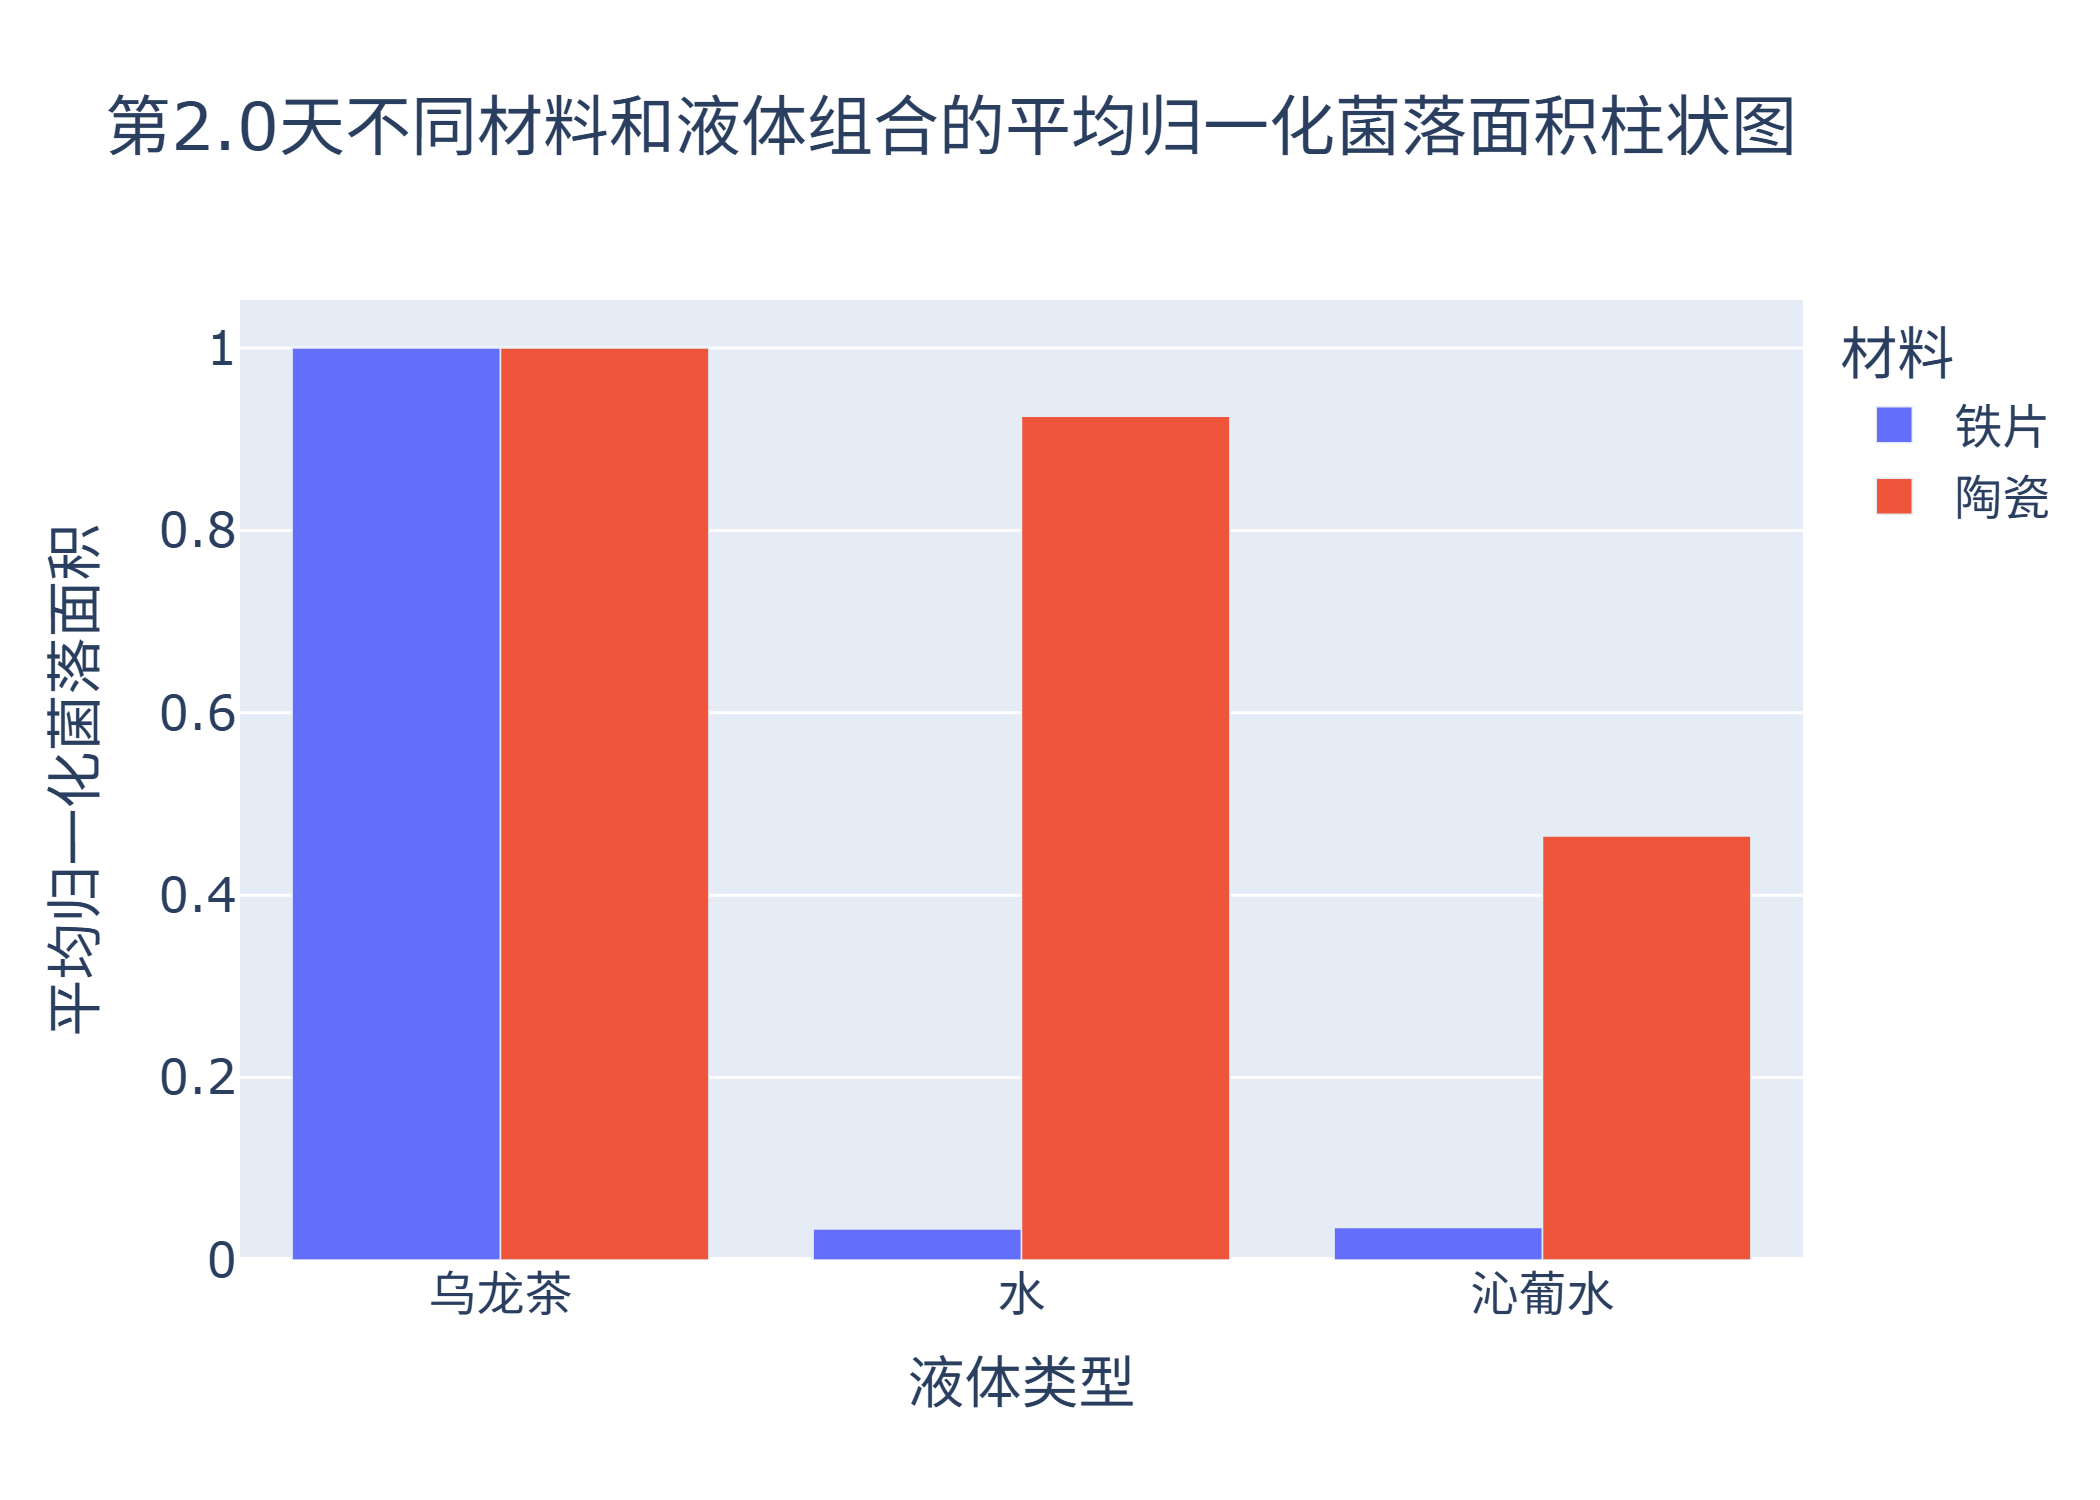
\includegraphics[width=\textwidth]{./plot/SingleDay/bar_normalized_day2.0.png}  % 替换为你的图片路径/文件名
    \caption{第二天}  % 图片标题
    \label{fig:SingleDayBar2}  % 标签,用于后文引用
\end{figure}

\begin{figure}[H]  % [H] 表示强制在此处插入(不浮动),也可用 htbp 等浮动选项
    \centering  % 图片居中显示
    % width=\textwidth 让图片宽度等于页面宽度(自动适应)
    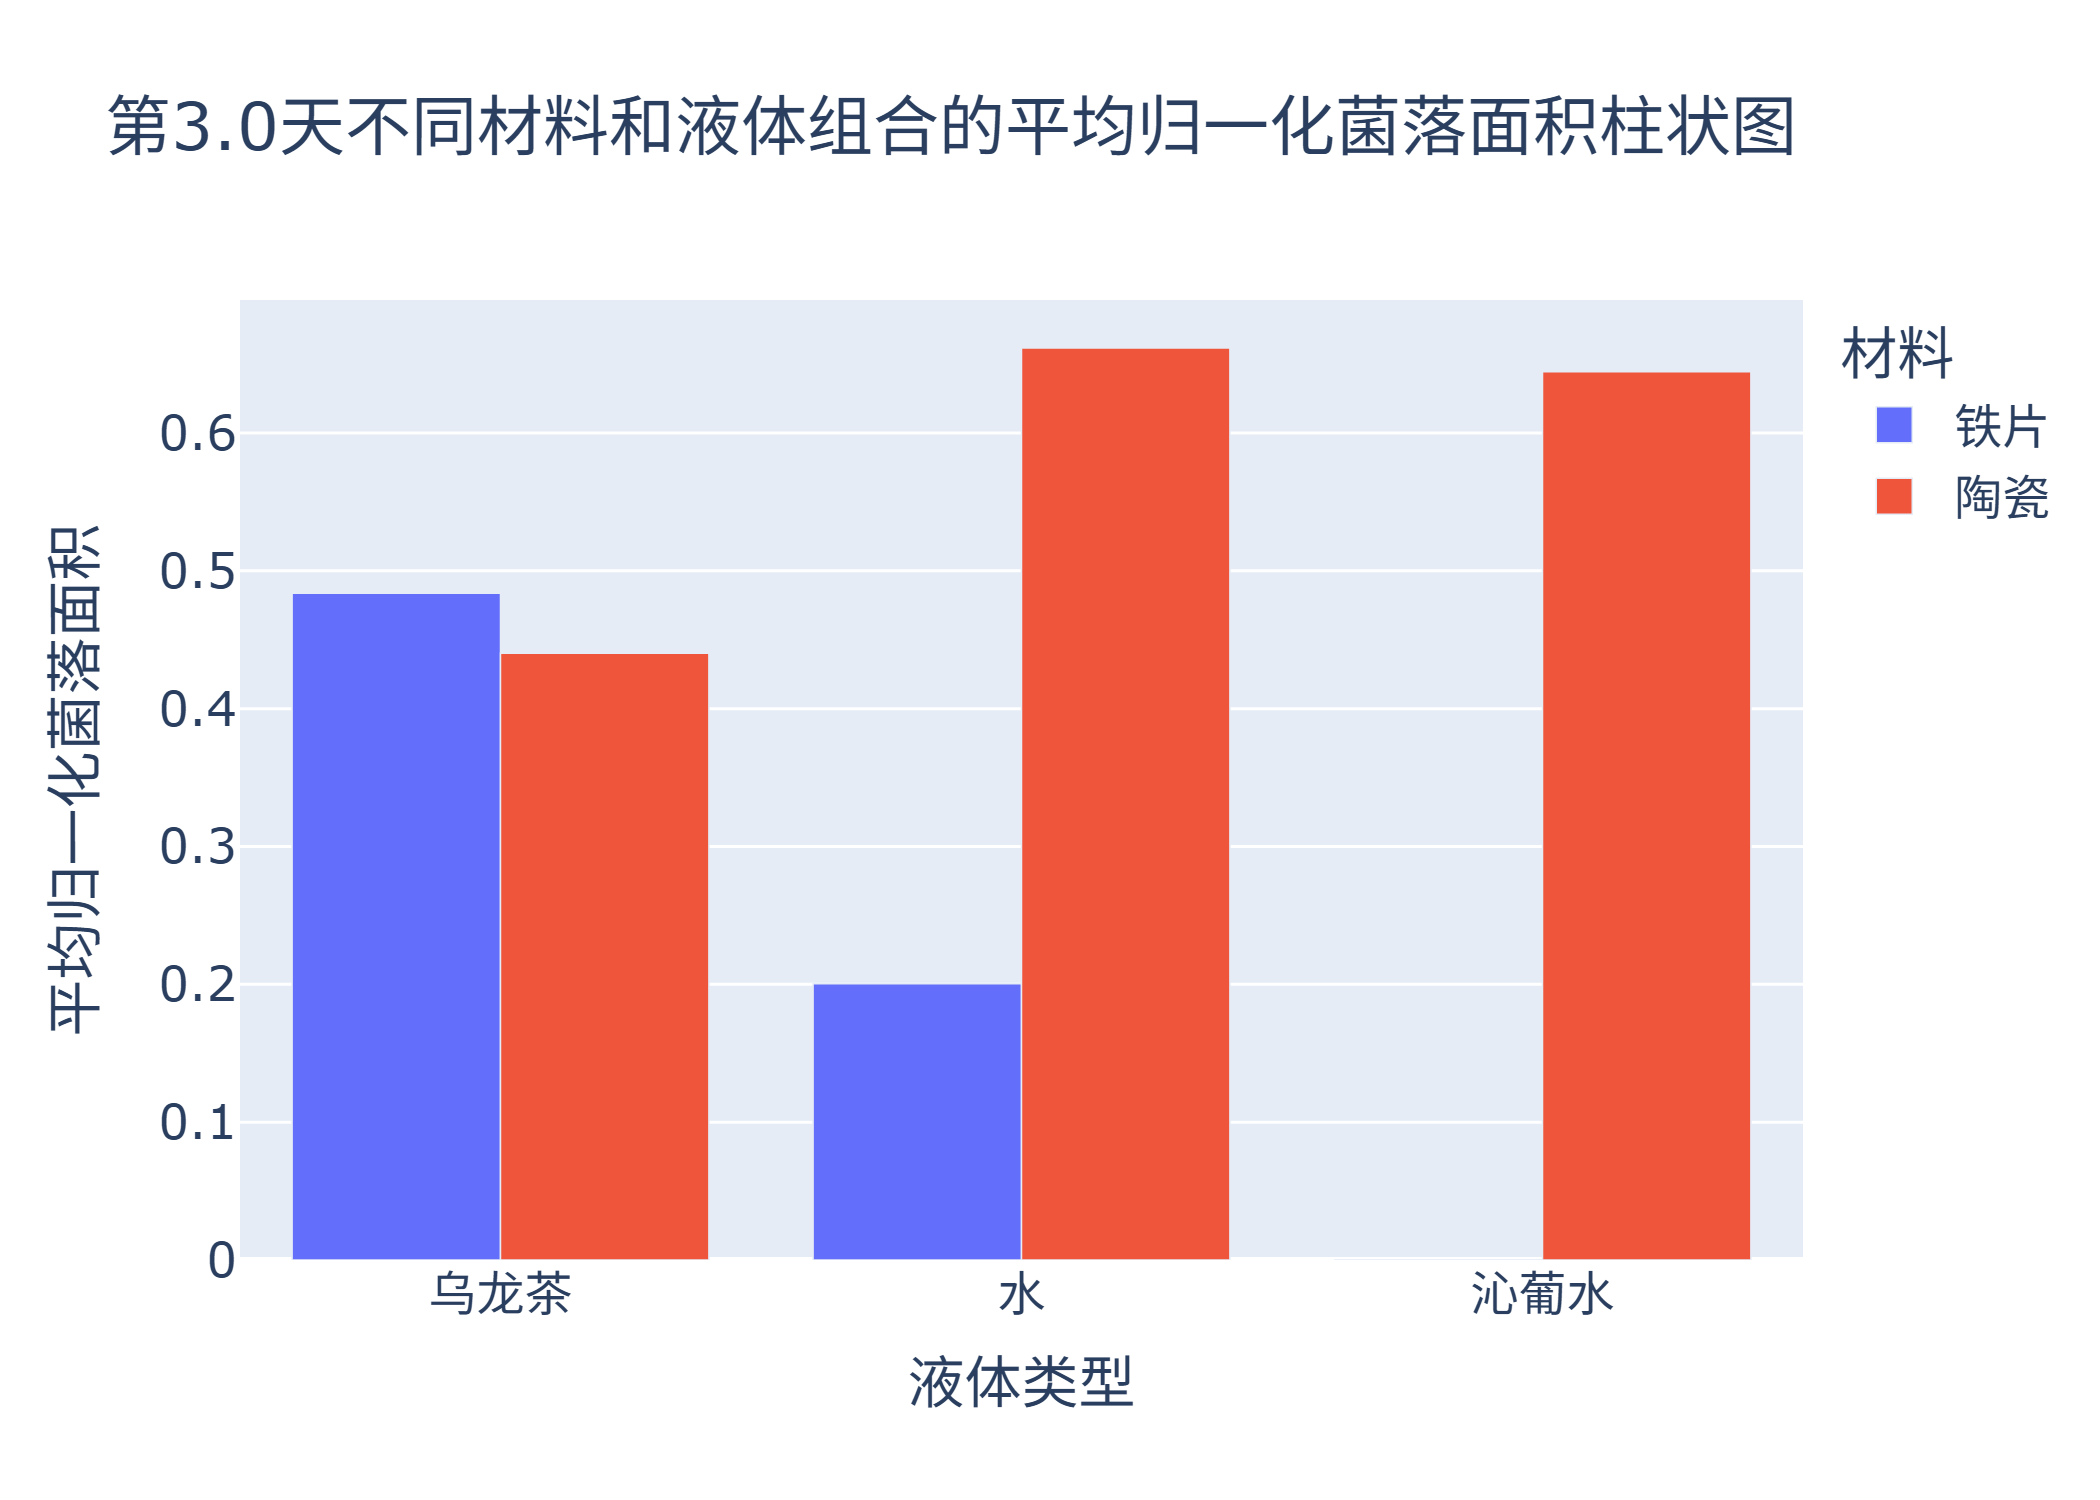
\includegraphics[width=\textwidth]{./plot/SingleDay/bar_normalized_day3.0.png}  % 替换为你的图片路径/文件名
    \caption{第三天}  % 图片标题
    \label{fig:SingleDayBar3}  % 标签,用于后文引用
\end{figure}

\begin{figure}[H]  % [H] 表示强制在此处插入(不浮动),也可用 htbp 等浮动选项
    \centering  % 图片居中显示
    % width=\textwidth 让图片宽度等于页面宽度(自动适应)
    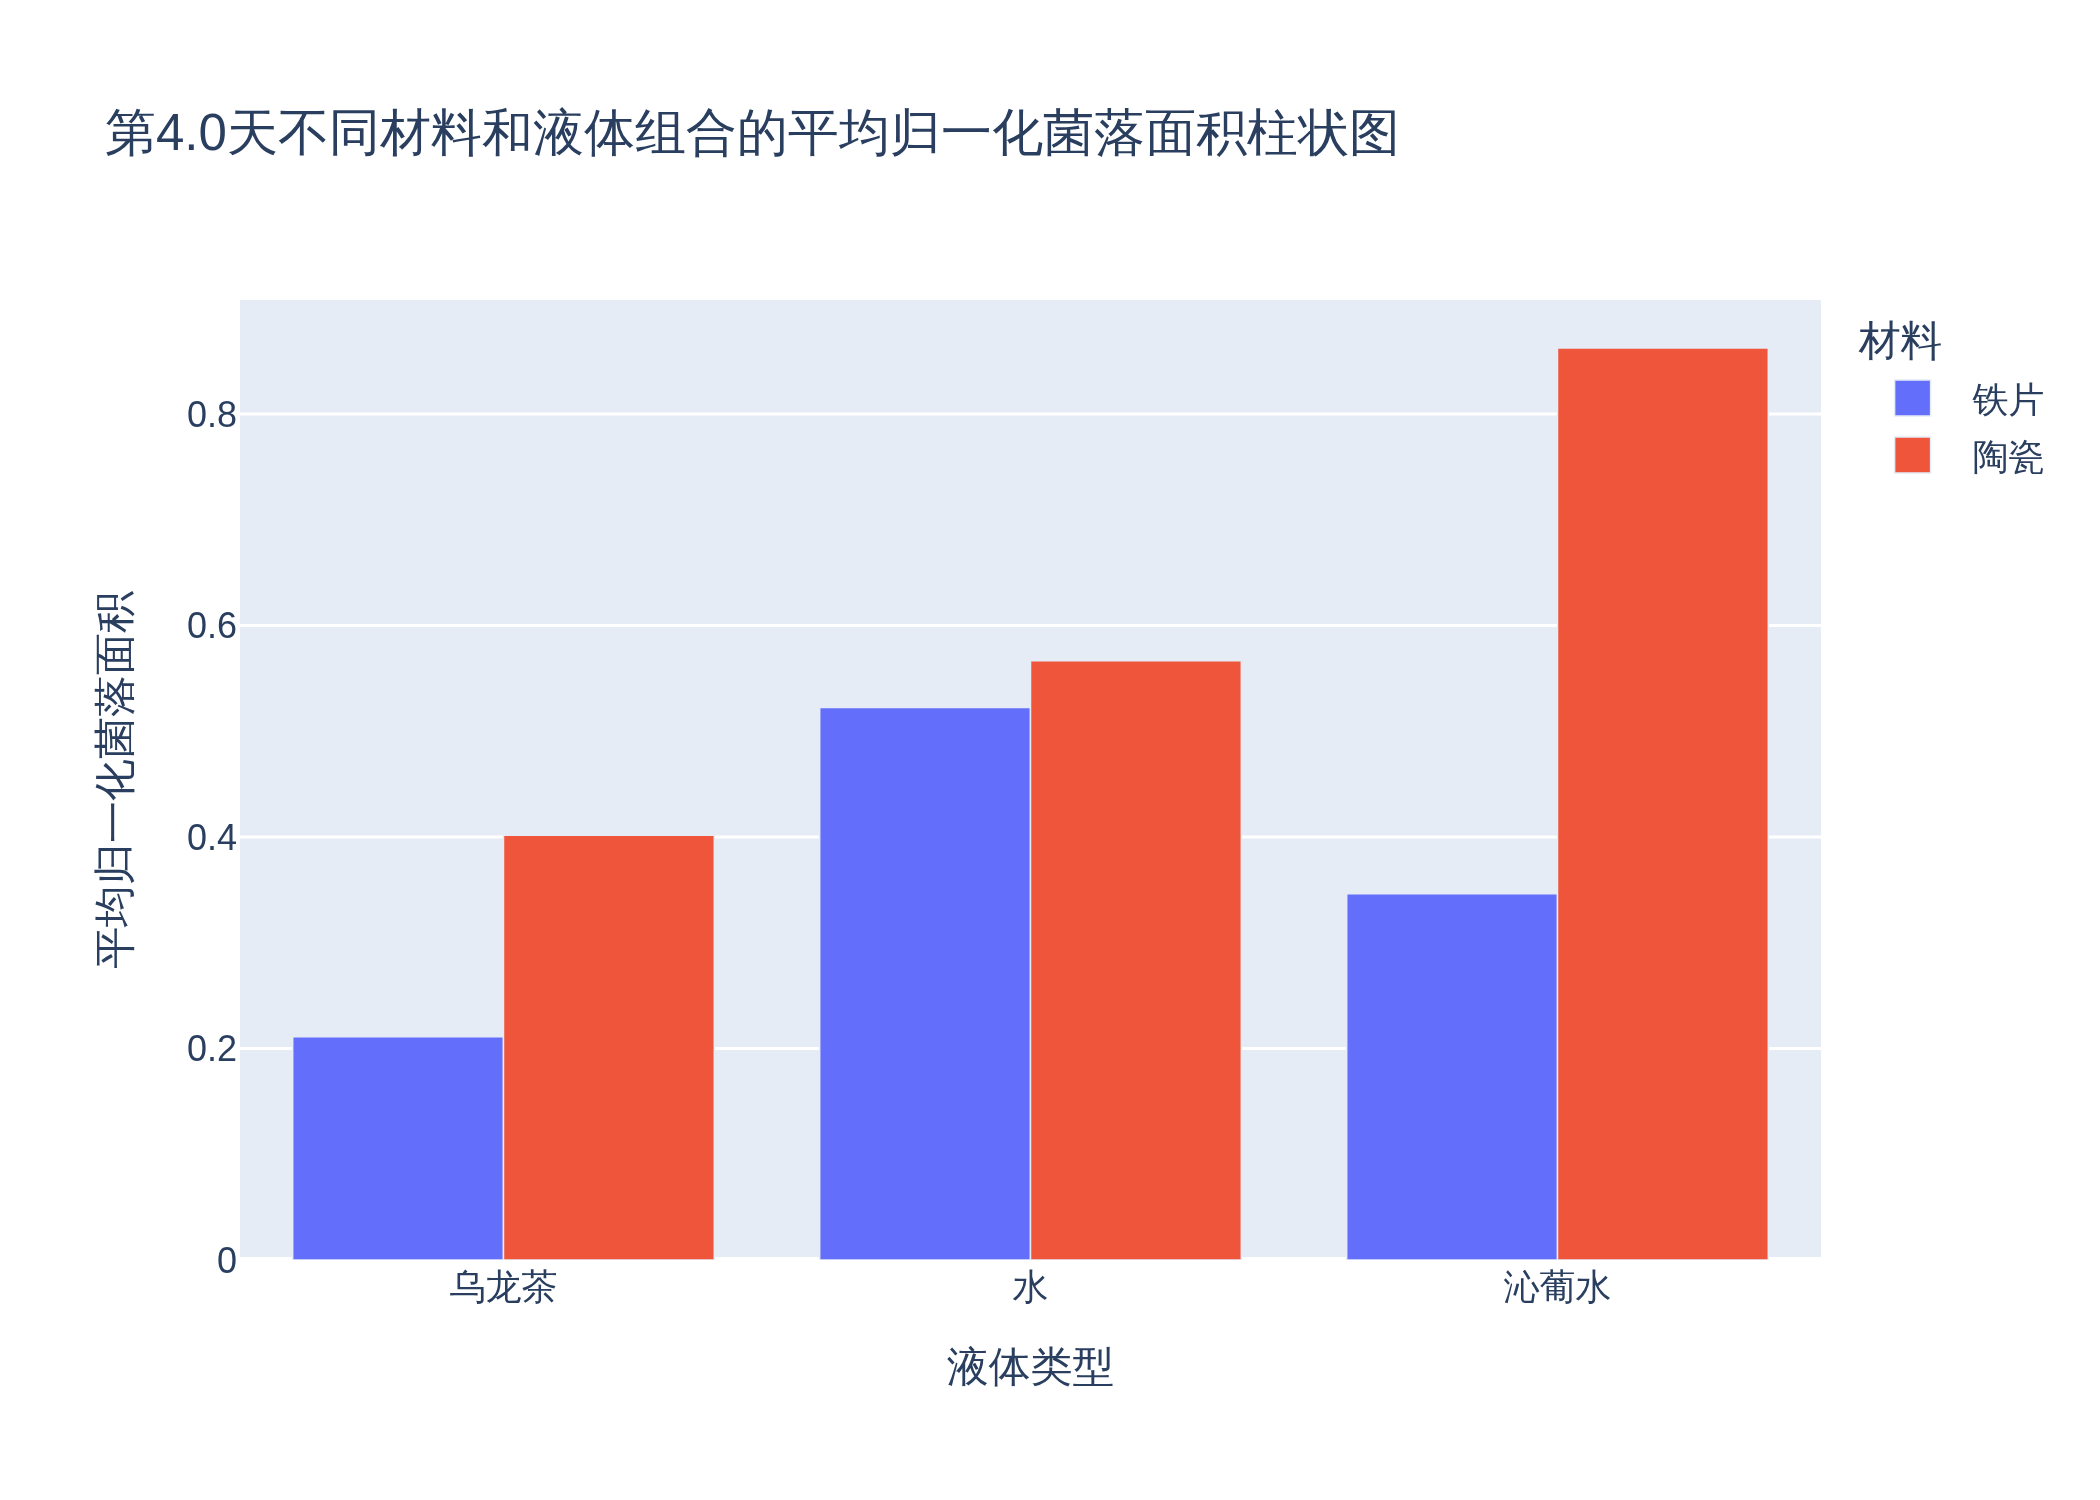
\includegraphics[width=\textwidth]{./plot/SingleDay/bar_normalized_day4.0.png}  % 替换为你的图片路径/文件名
    \caption{第四天}  % 图片标题
    \label{fig:SingleDayBar4}  % 标签,用于后文引用
\end{figure}

\begin{figure}[H]  % [H] 表示强制在此处插入(不浮动),也可用 htbp 等浮动选项
    \centering  % 图片居中显示
    % width=\textwidth 让图片宽度等于页面宽度(自动适应)
    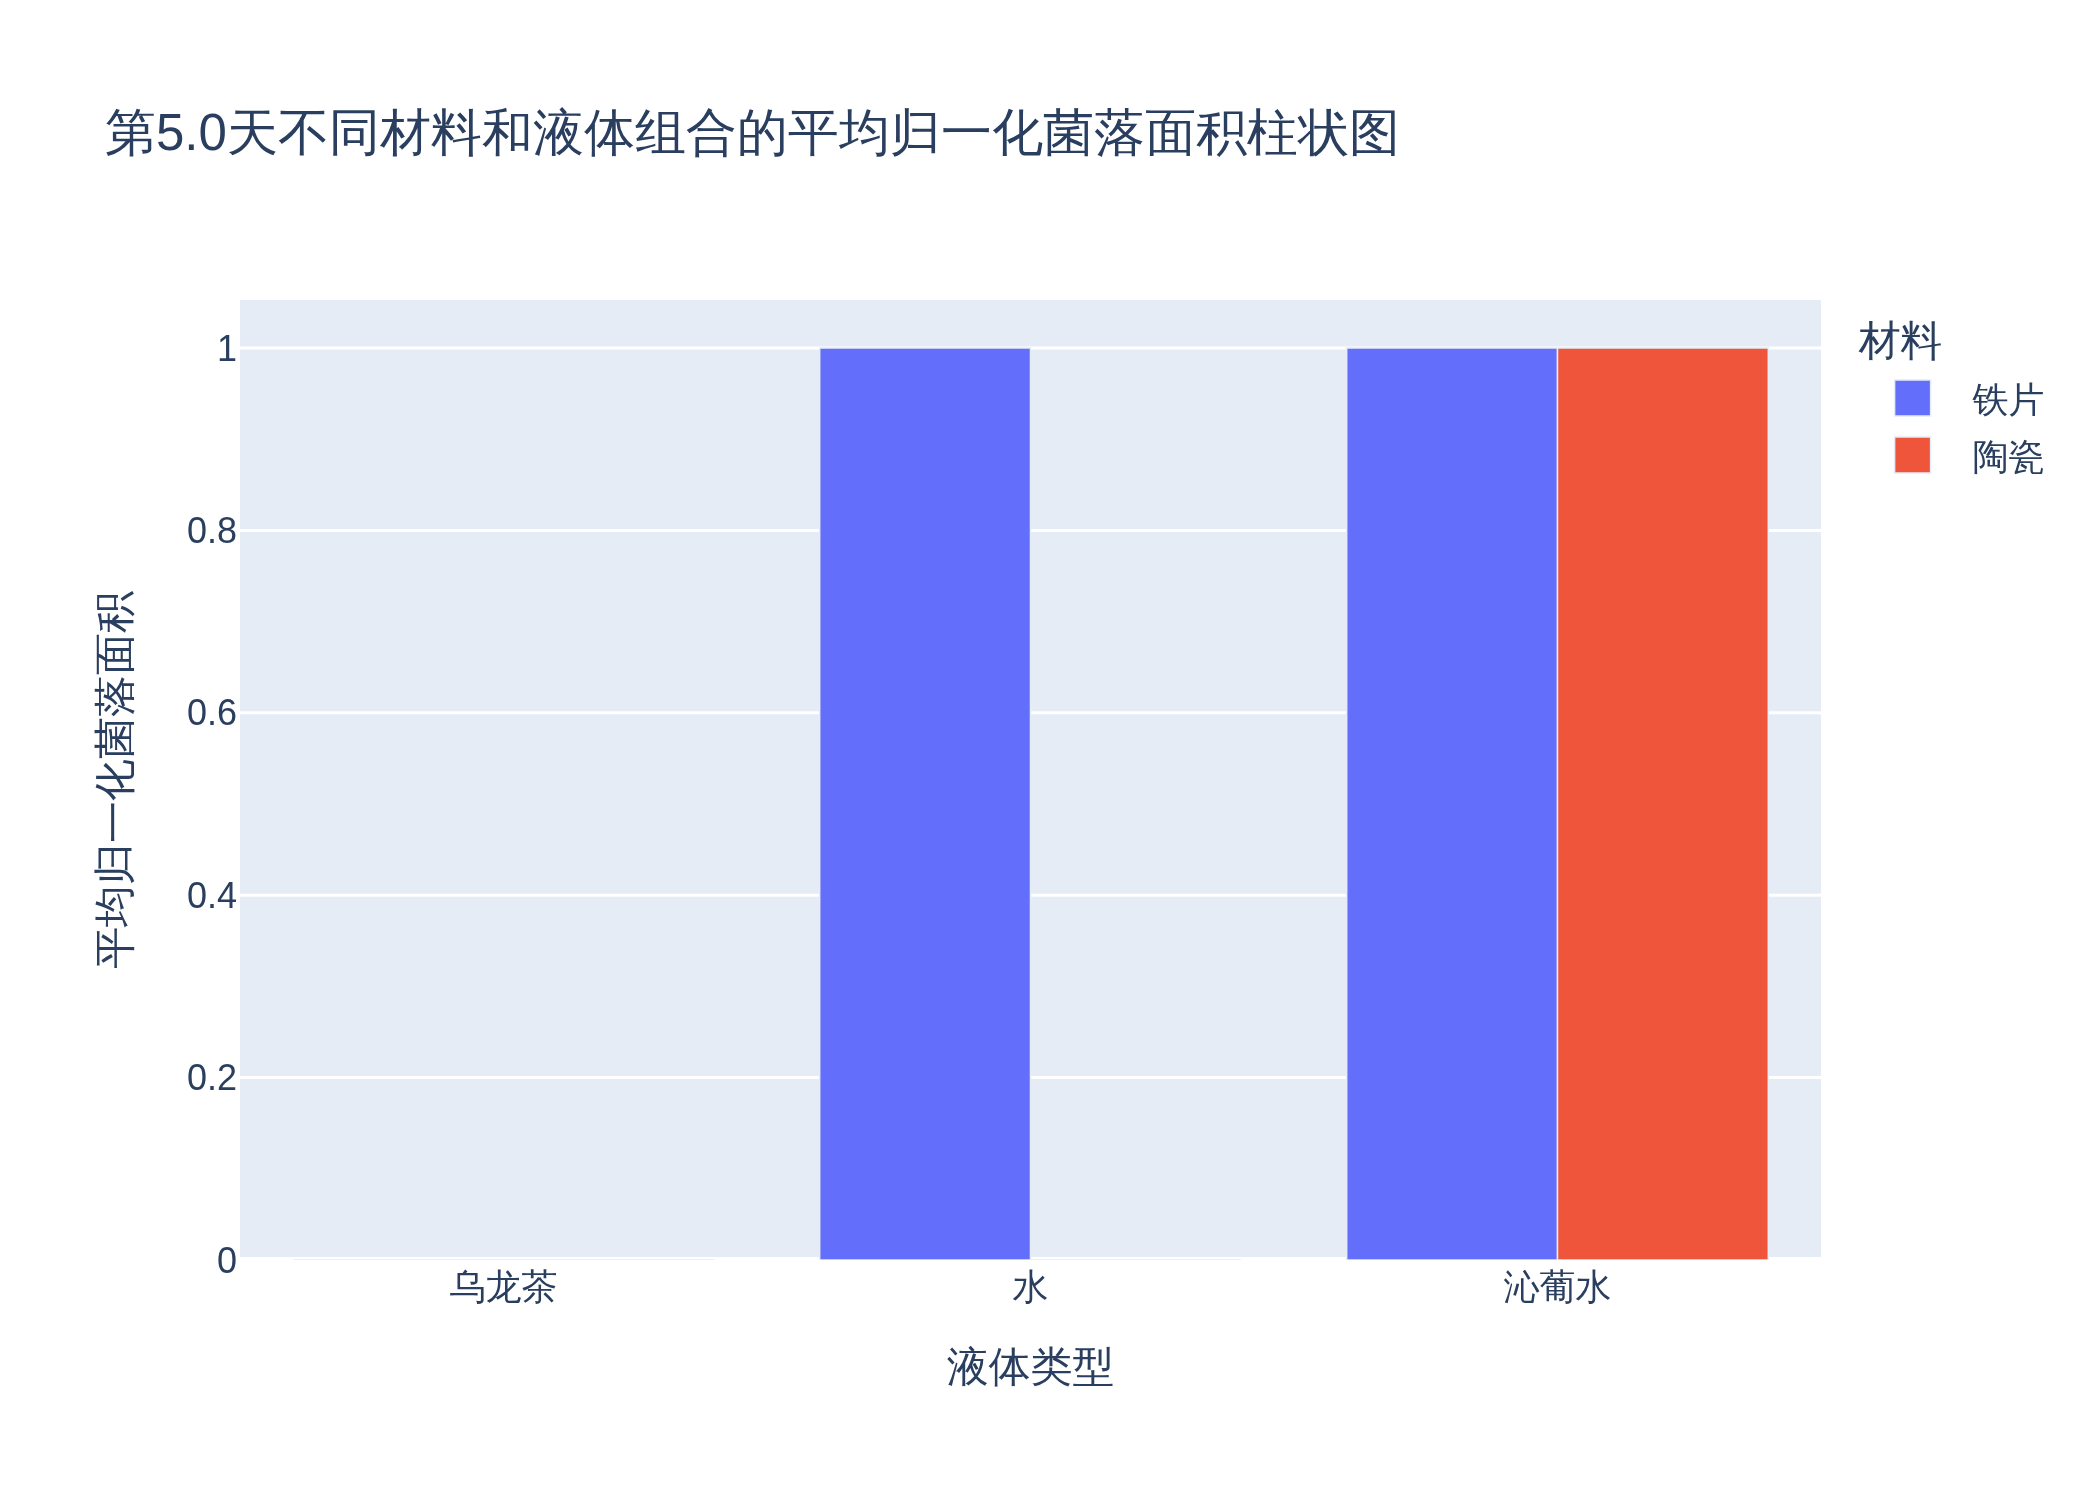
\includegraphics[width=\textwidth]{./plot/SingleDay/bar_normalized_day5.0.png}  % 替换为你的图片路径/文件名
    \caption{第五天}  % 图片标题
    \label{fig:SingleDayBar5}  % 标签,用于后文引用
\end{figure}
\subsection{天数相同,材料、溶液不同的归一化热力图}
\begin{figure}[H]  % [H] 表示强制在此处插入(不浮动),也可用 htbp 等浮动选项
    \centering  % 图片居中显示
    % width=\textwidth 让图片宽度等于页面宽度(自动适应)
    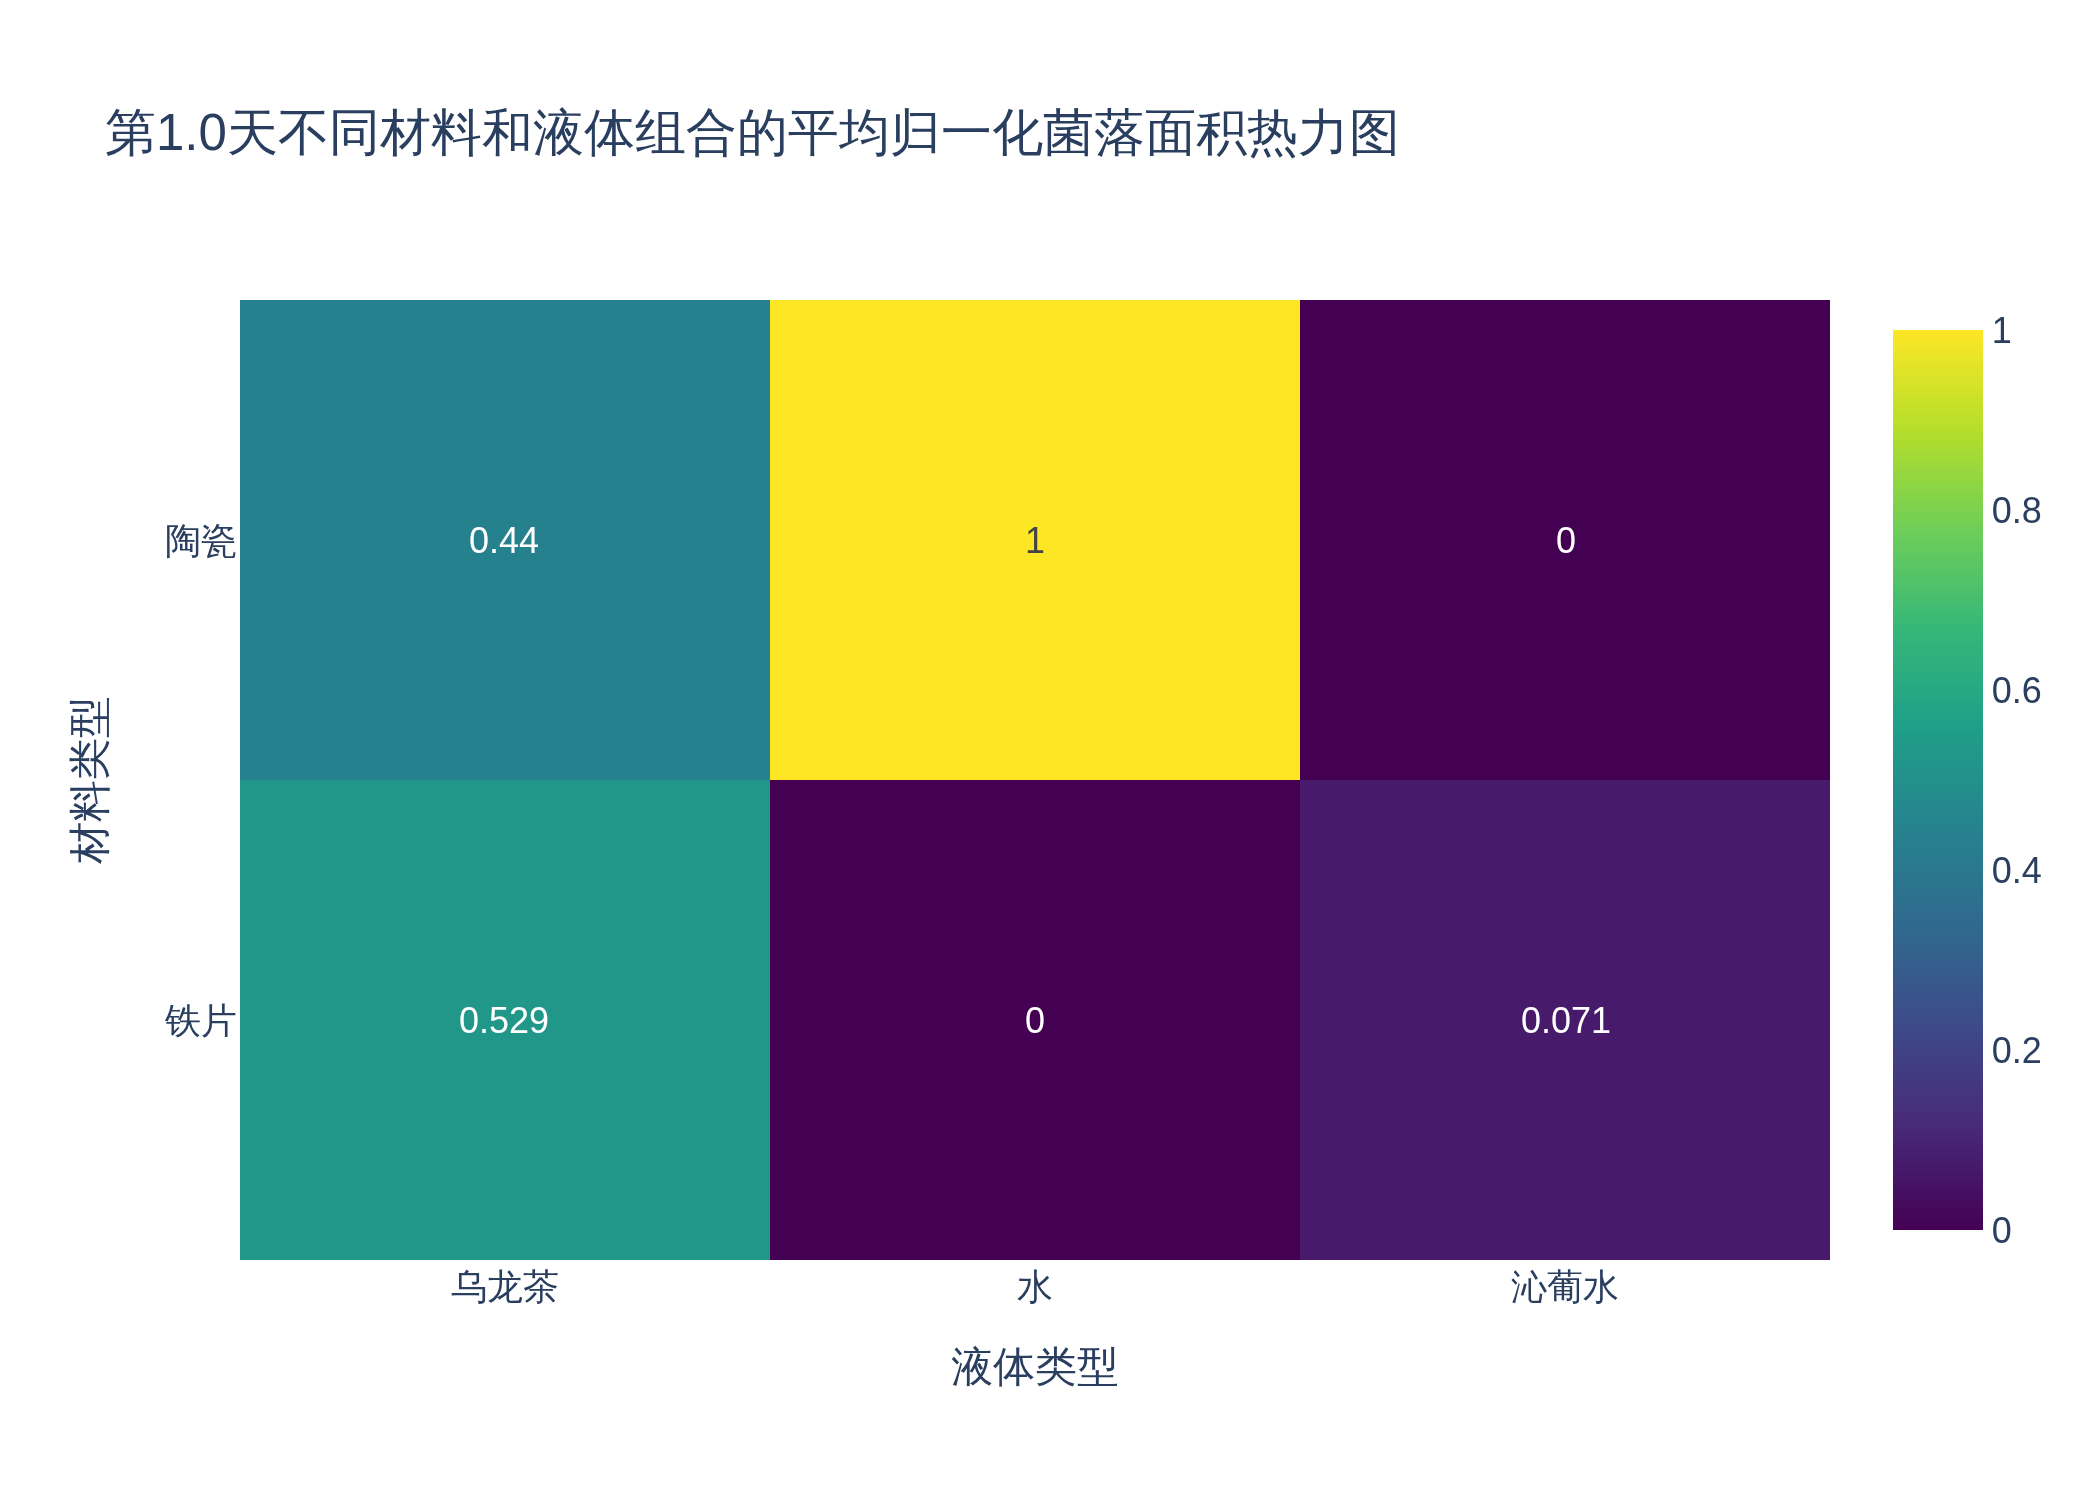
\includegraphics[width=\textwidth]{./plot/SingleDay/heatmap_normalized_day1.0.png}  % 替换为你的图片路径/文件名
    \caption{第一天}  % 图片标题
    \label{fig:SingleDayHeat1}  % 标签,用于后文引用
\end{figure}

\begin{figure}[H]  % [H] 表示强制在此处插入(不浮动),也可用 htbp 等浮动选项
    \centering  % 图片居中显示
    % width=\textwidth 让图片宽度等于页面宽度(自动适应)
    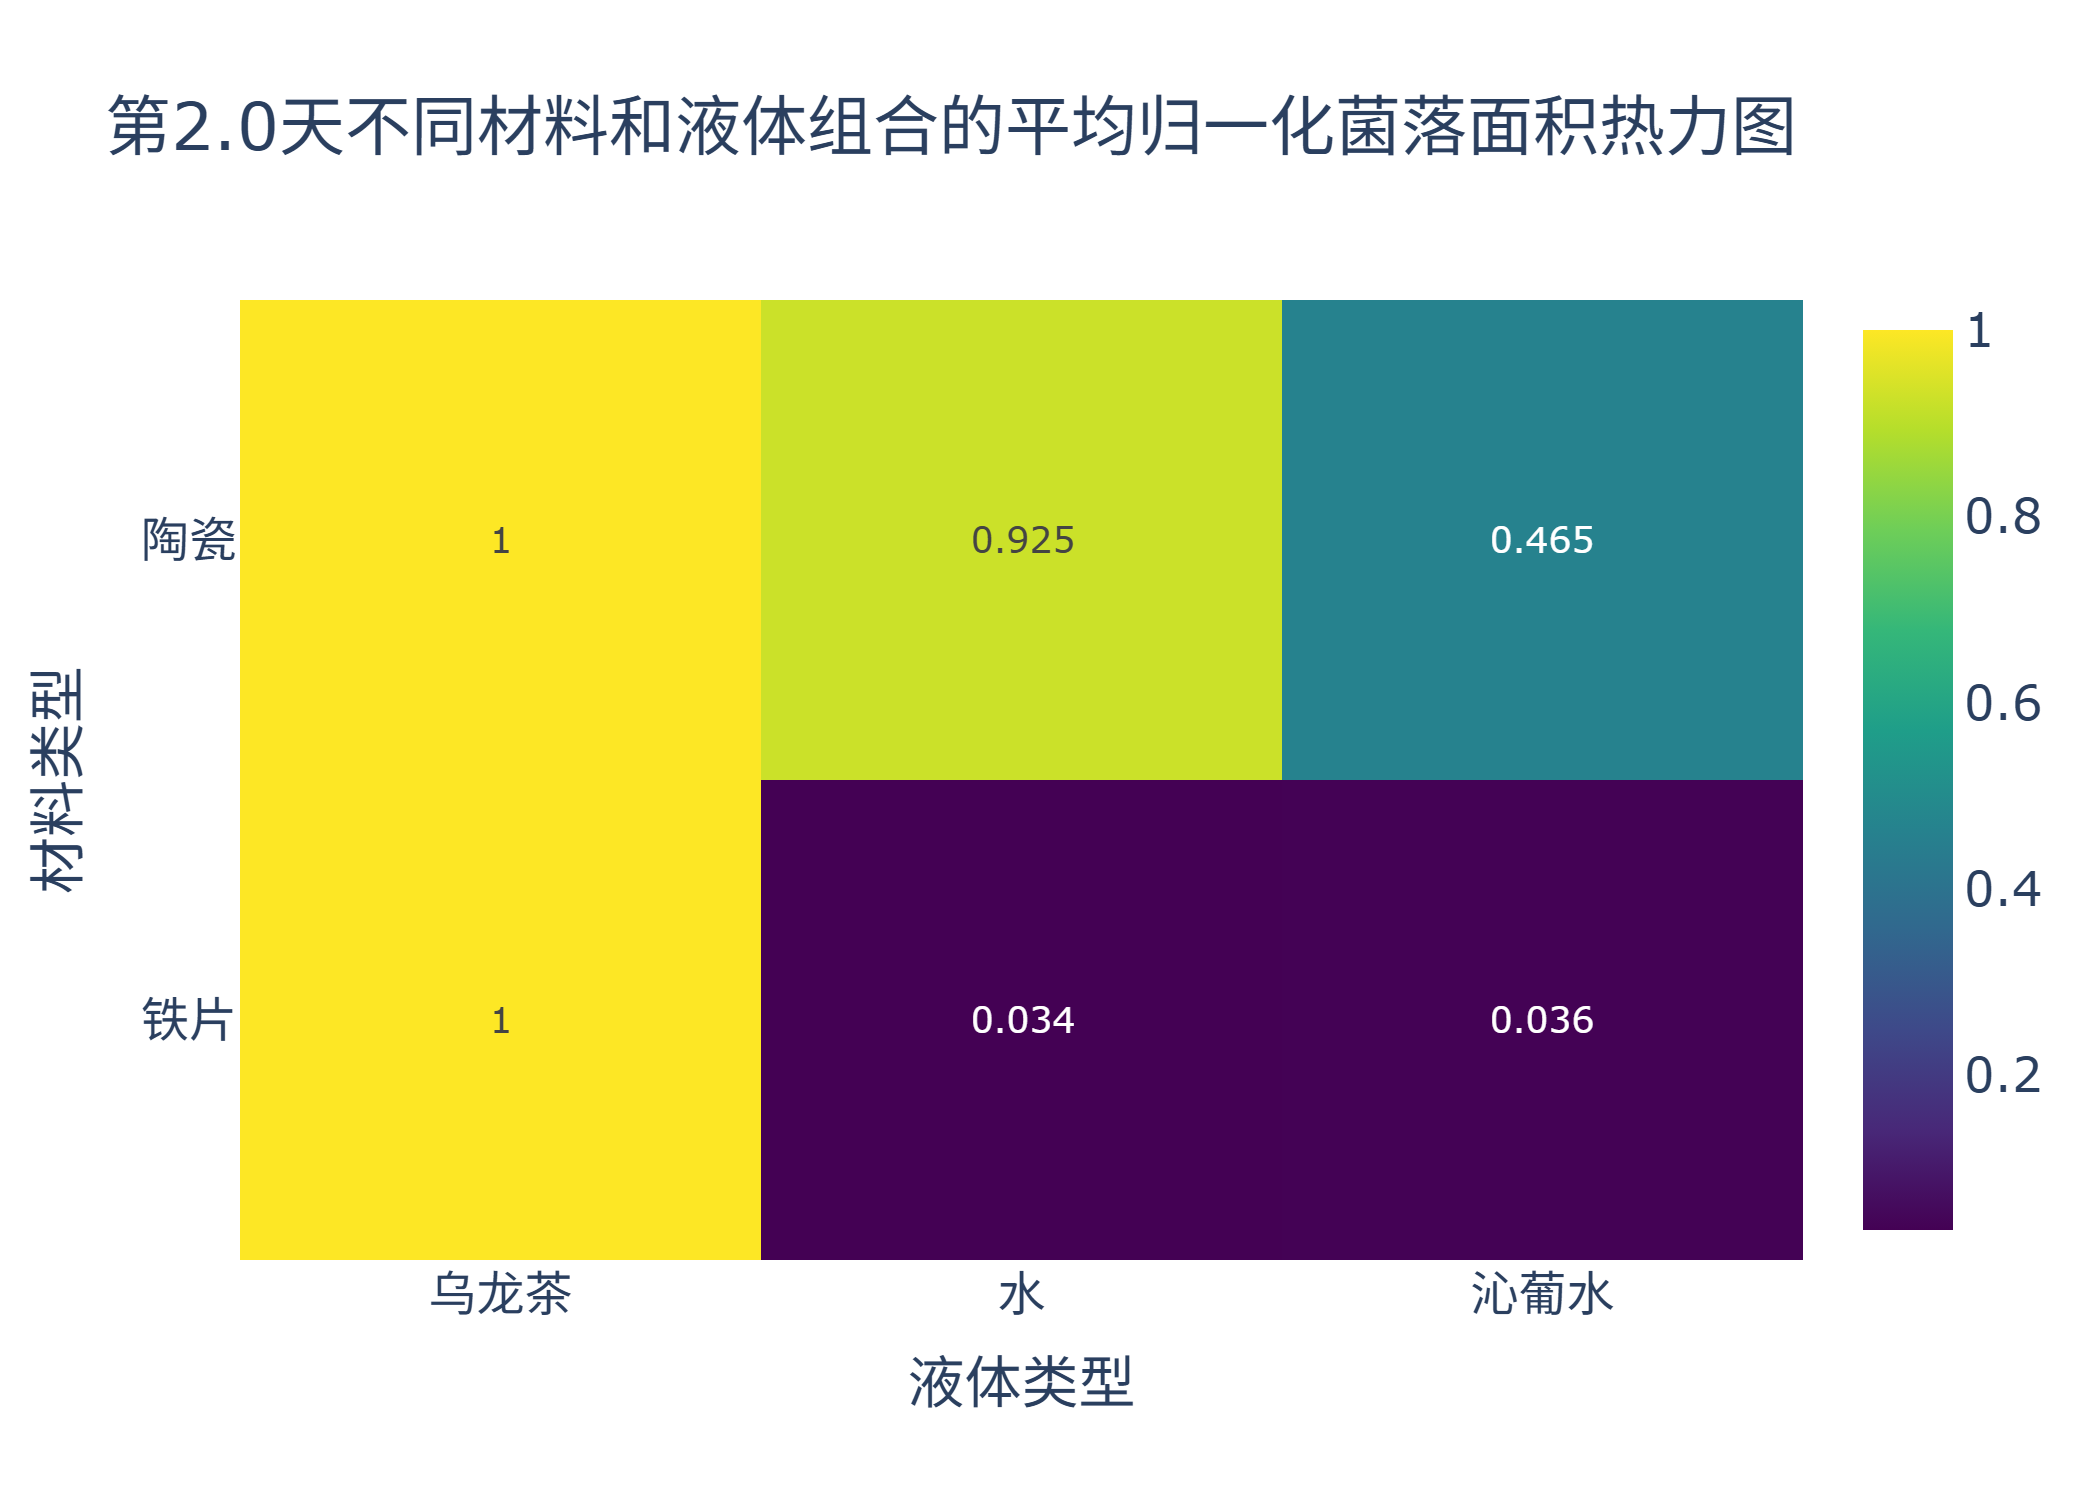
\includegraphics[width=\textwidth]{./plot/SingleDay/heatmap_normalized_day2.0.png}  % 替换为你的图片路径/文件名
    \caption{第二天}  % 图片标题
    \label{fig:SingleDayHeat2}  % 标签,用于后文引用
\end{figure}

\begin{figure}[H]  % [H] 表示强制在此处插入(不浮动),也可用 htbp 等浮动选项
    \centering  % 图片居中显示
    % width=\textwidth 让图片宽度等于页面宽度(自动适应)
    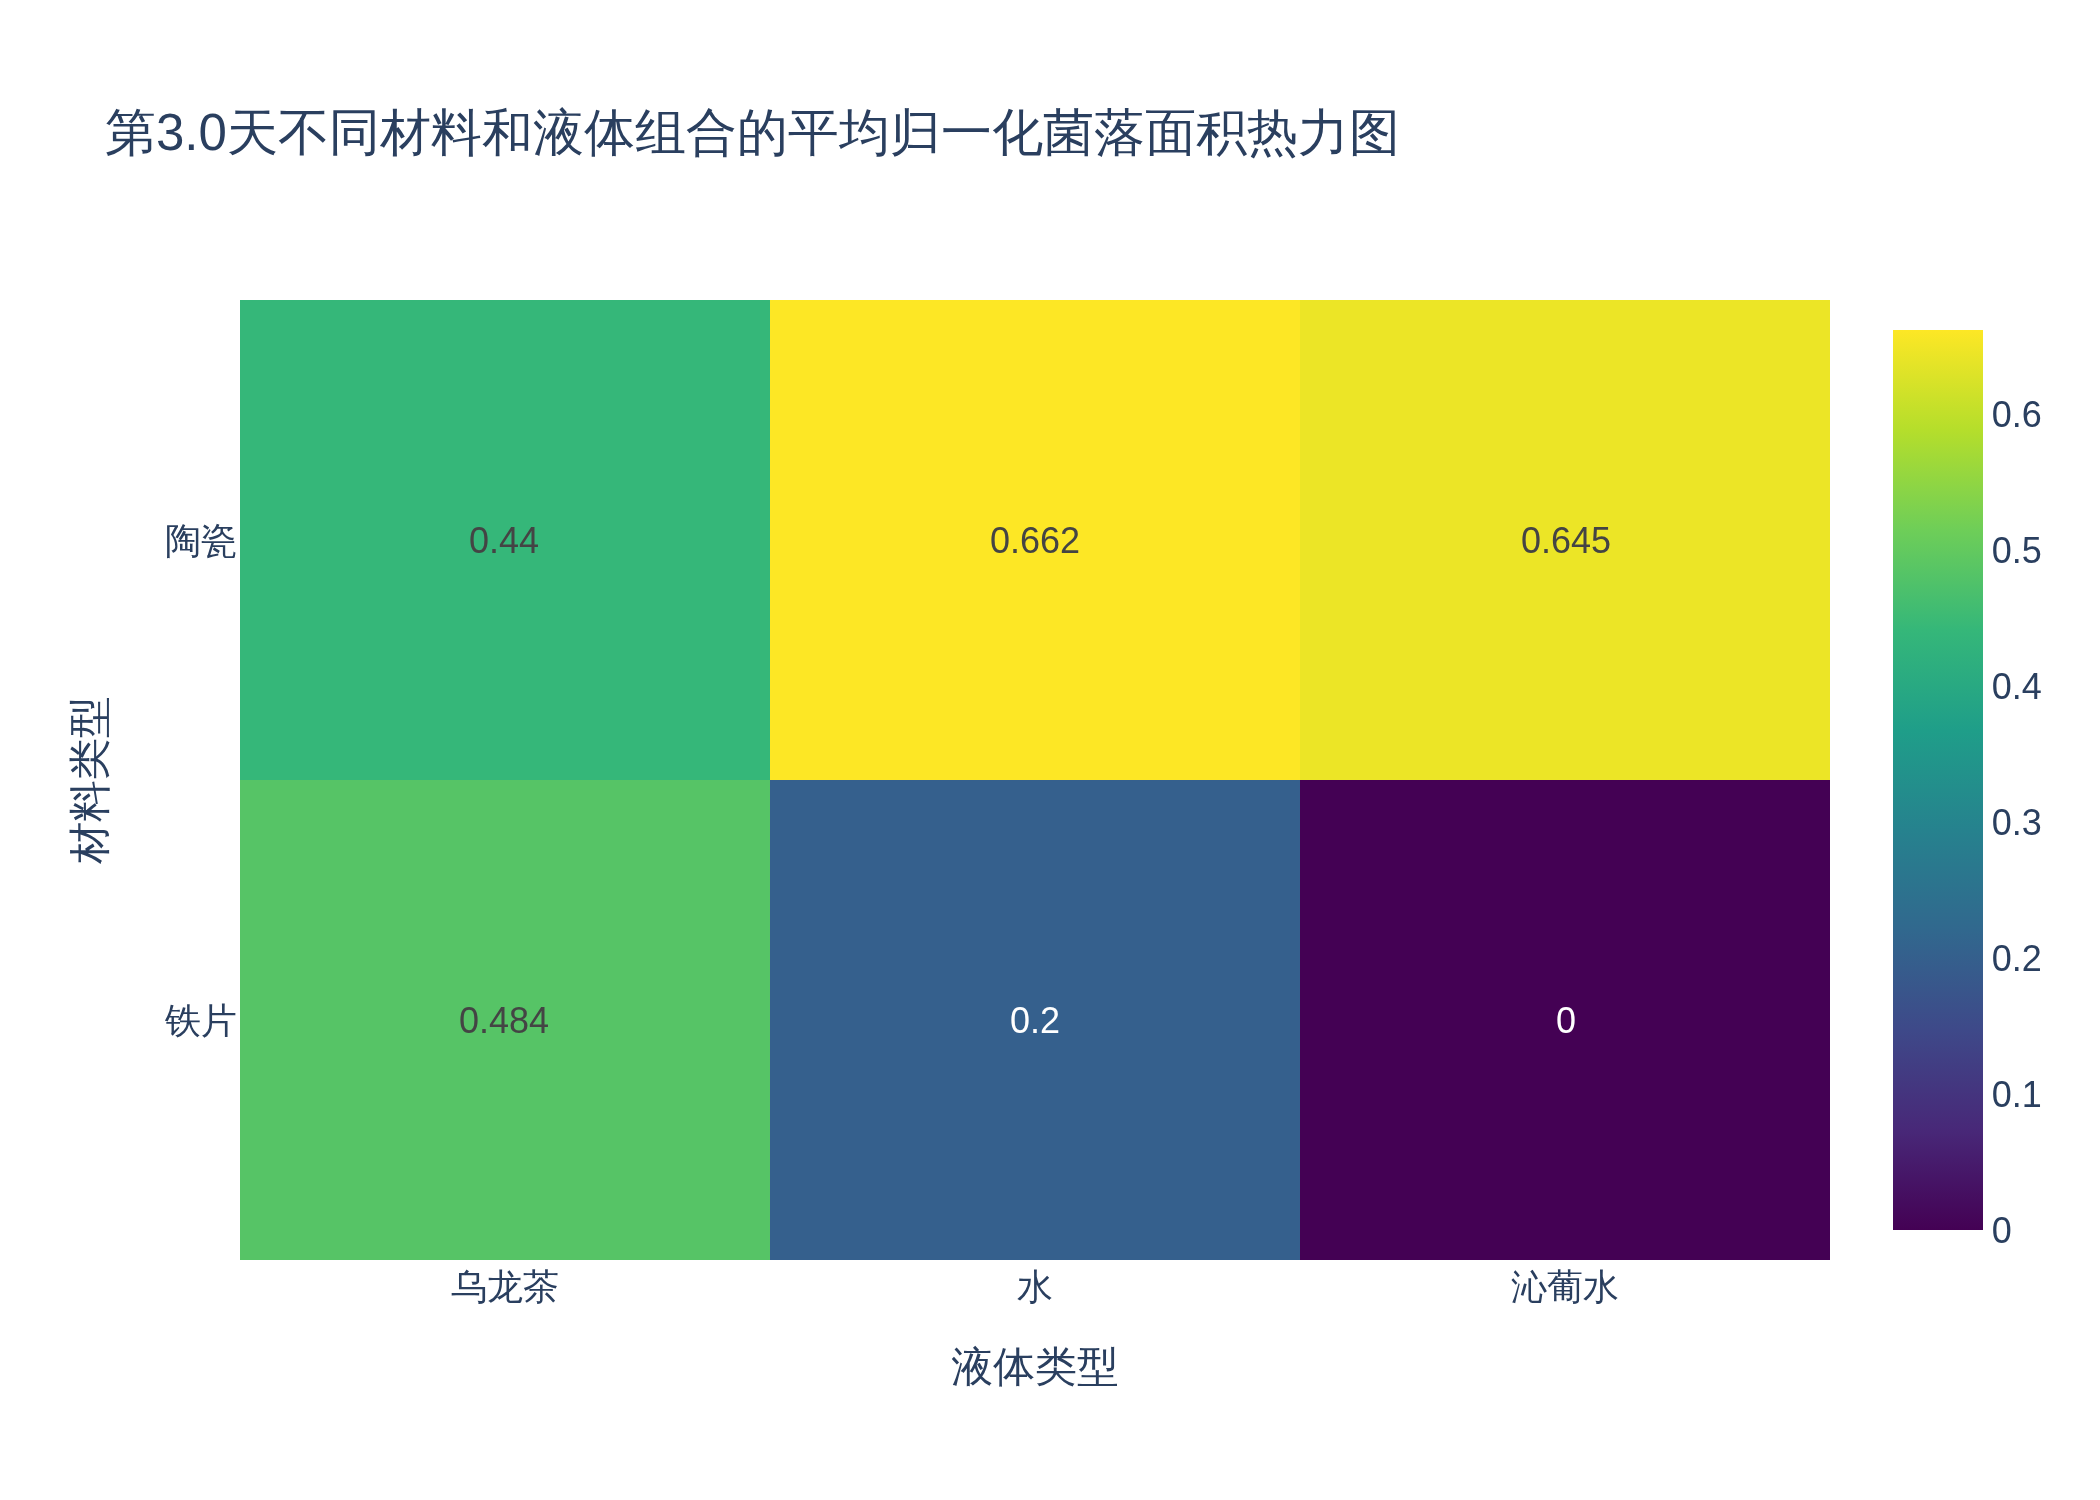
\includegraphics[width=\textwidth]{./plot/SingleDay/heatmap_normalized_day3.0.png}  % 替换为你的图片路径/文件名
    \caption{第三天}  % 图片标题
    \label{fig:SingleDayHeat3}  % 标签,用于后文引用
\end{figure}

\begin{figure}[H]  % [H] 表示强制在此处插入(不浮动),也可用 htbp 等浮动选项
    \centering  % 图片居中显示
    % width=\textwidth 让图片宽度等于页面宽度(自动适应)
    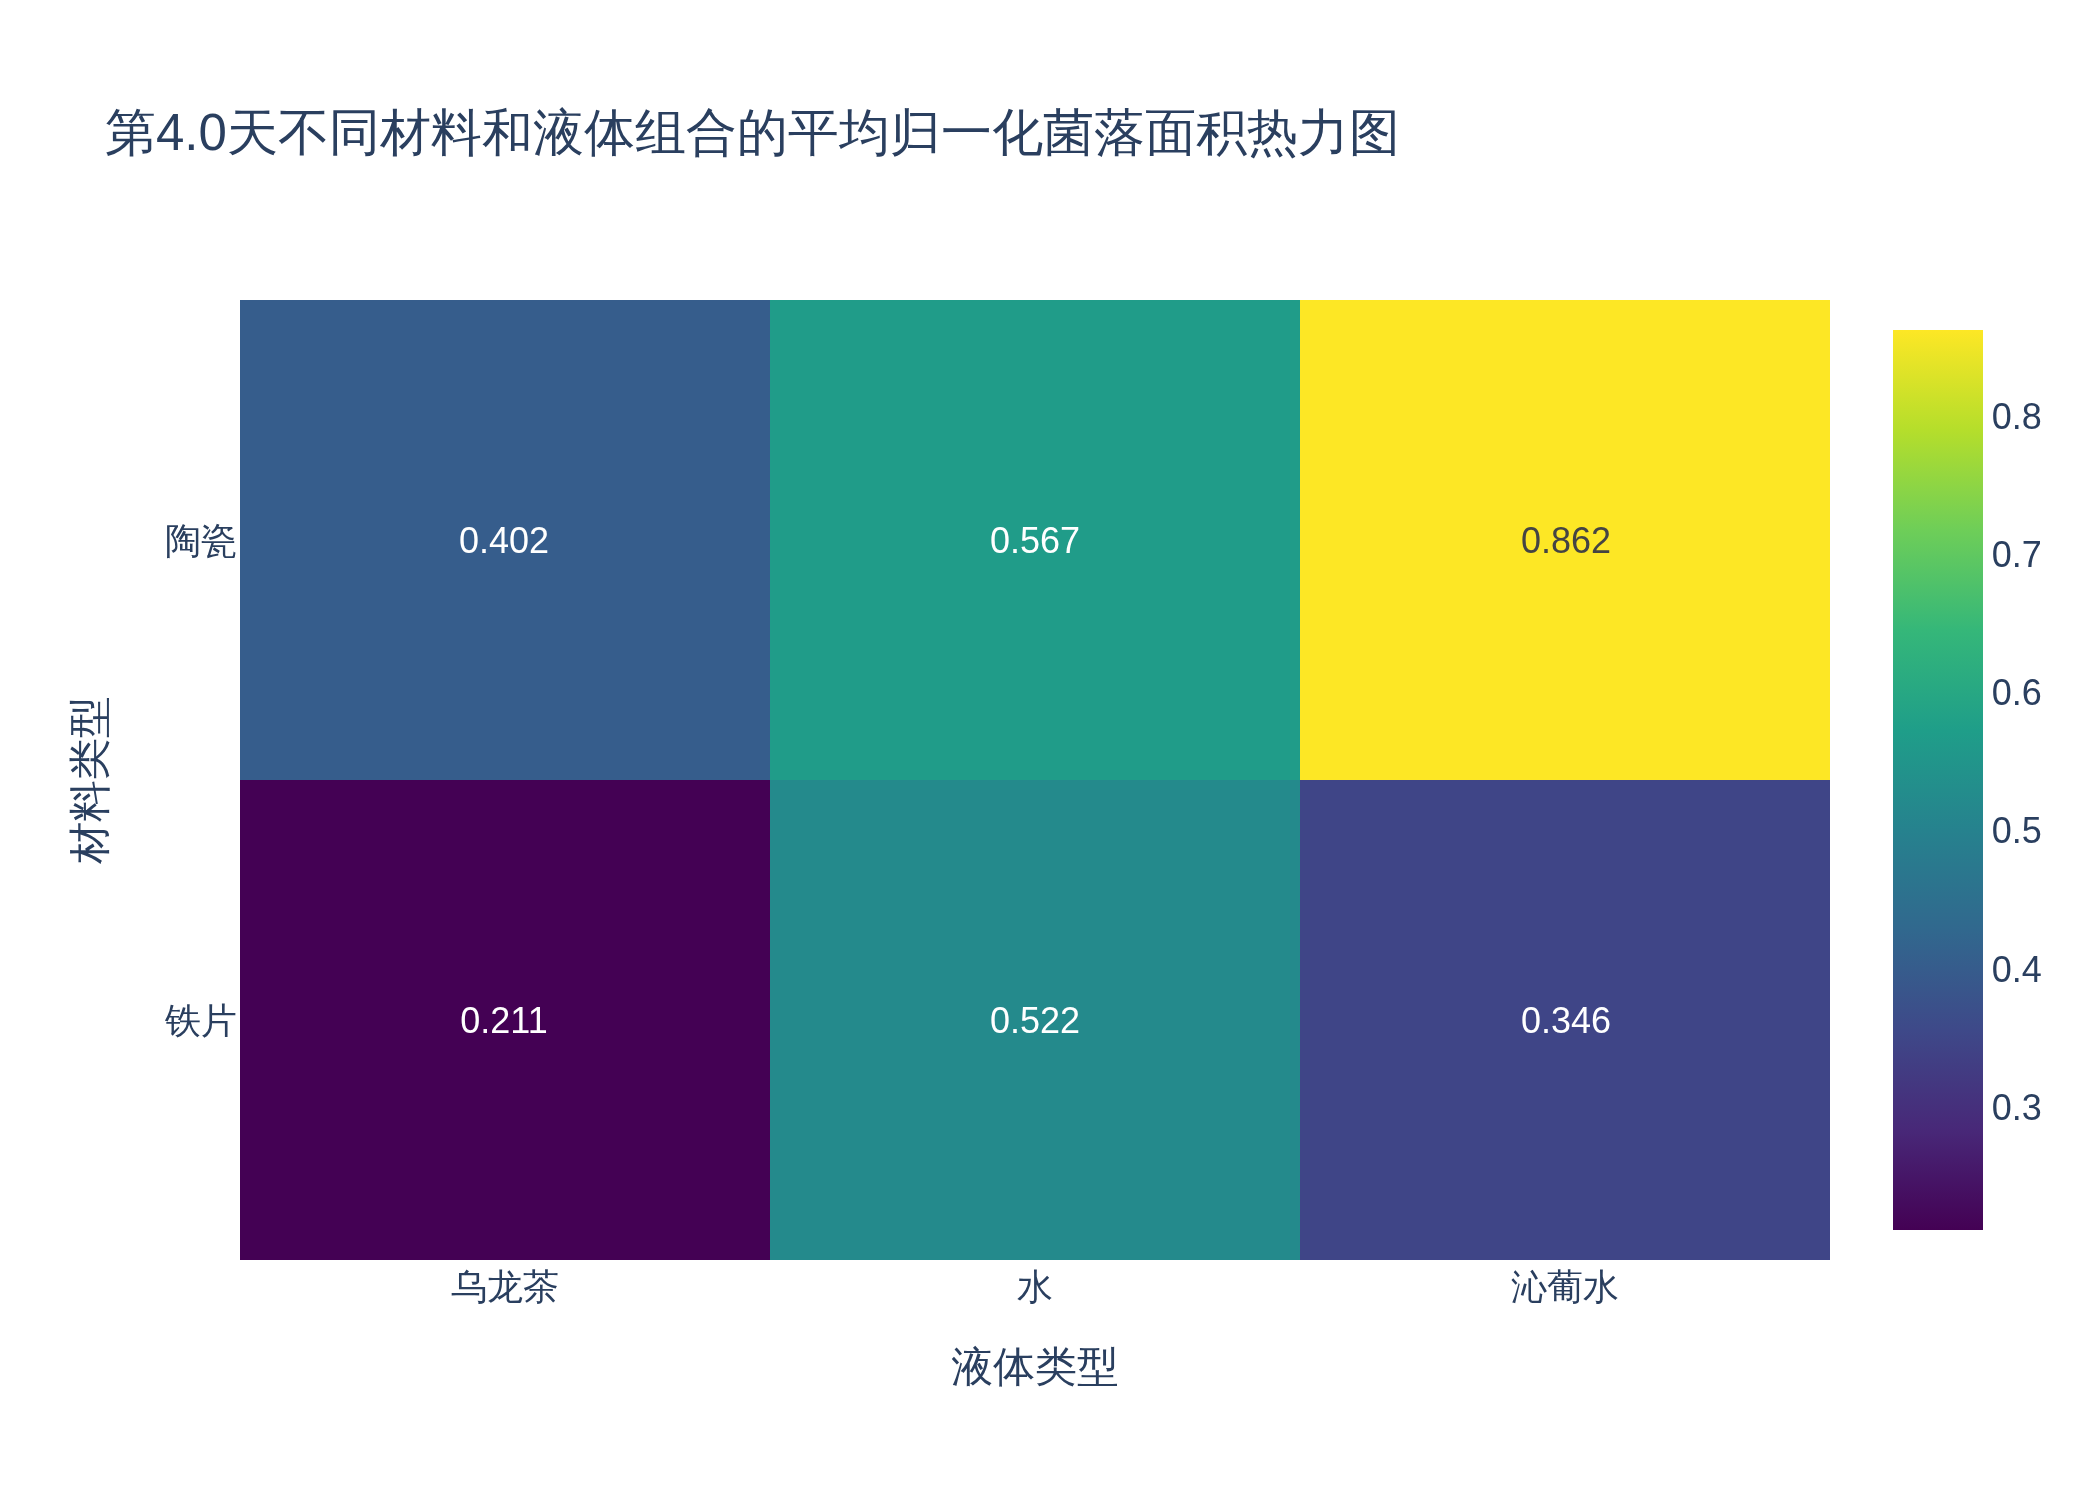
\includegraphics[width=\textwidth]{./plot/SingleDay/heatmap_normalized_day4.0.png}  % 替换为你的图片路径/文件名
    \caption{第四天}  % 图片标题
    \label{fig:SingleDayHeat4}  % 标签,用于后文引用
\end{figure}

\begin{figure}[H]  % [H] 表示强制在此处插入(不浮动),也可用 htbp 等浮动选项
    \centering  % 图片居中显示
    % width=\textwidth 让图片宽度等于页面宽度(自动适应)
    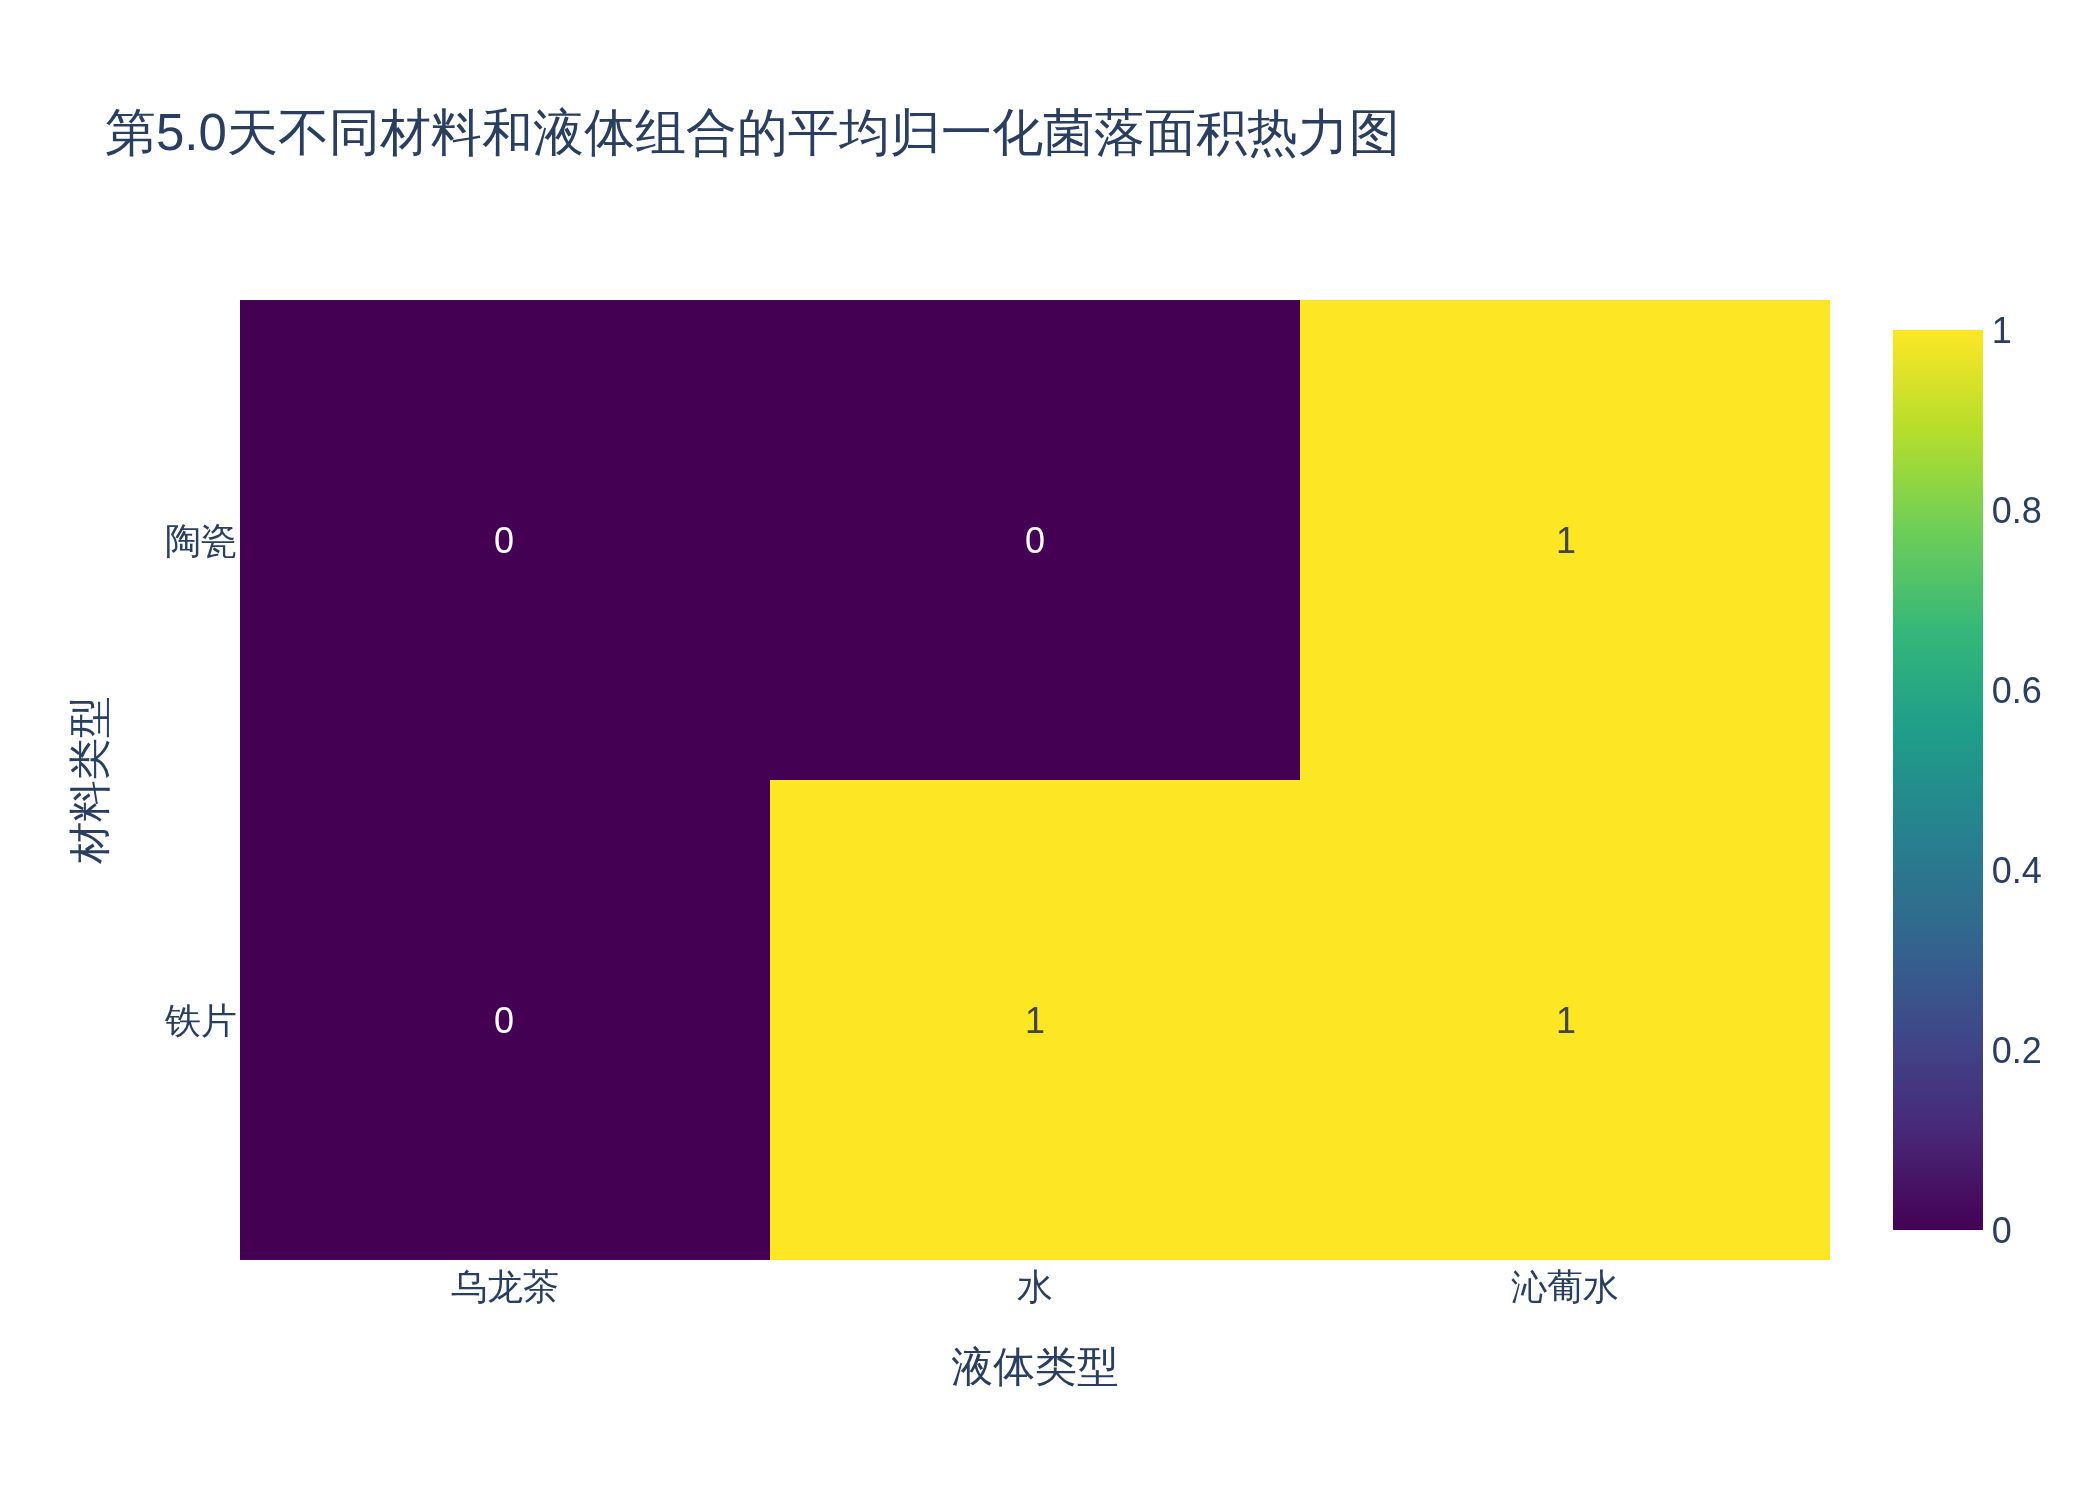
\includegraphics[width=\textwidth]{./plot/SingleDay/heatmap_normalized_day5.0.png}  % 替换为你的图片路径/文件名
    \caption{第五天}  % 图片标题
    \label{fig:SingleDayHeat5}  % 标签,用于后文引用
\end{figure}
\newpage

\clearpage
\thispagestyle{empty}
\section{附录B:相关数据及修正}
由于此处篇幅有限,故不插入完整的数据表格,该数据来自源数据的平均值。
\begin{longtable}{c c c c c c}
  \caption{陶瓷材质与不同液体组合的相关数据} \\
  \toprule
  \textbf{液体类型} & 天数 & 实际值 & 偏置项 & 修正方式 & 最终结果 \\
  \midrule
  \endfirsthead  % 首页表头(跨页时显示)
  
  \caption*{续表:陶瓷材质与不同液体组合的相关数据} \\
  \toprule
  \textbf{液体类型} & 天数 & 实际值 & 偏置项 & 修正方式 & 最终结果 \\
  \midrule
  \endhead  % 后续页表头(跨页时显示)
  
  \bottomrule
  \endlastfoot  % 末页表尾(跨页时显示)

  % 第一组:陶瓷-水(用\multirow合并多行,标注液体类型)
  \multirow{5}{*}{水} 
    & 1 & 195      & 450    & 偏置      & 645      \\
    & 2 & 151.8    & 450    & 偏置       & 601.8    \\
    & 3 & 0        & 450    & 偏置     & 450      \\
    & 4 & 845.25   & -450   & 偏置     & 395.25   \\
    & 5 & 518.6    & -450   & 偏置     & 68.6     \\
  \midrule
  
  % 第二组:陶瓷-沁葡水
  \multirow{5}{*}{沁葡水} 
    & 1 & 0        & 0      & 无     & 0        \\
    & 2 & 2204.61  & 0      & 无     & 2204.61  \\
    & 3 & 3056.33  & 0      & 无     & 3056.33  \\
    & 4 & 89.29    & -   & 错误数据     & -  \\
    & 5 & 4742.14  & 0      & 无       & 4742.14  \\
  \midrule
  
  % 第三组:陶瓷-乌龙茶
  \multirow{5}{*}{乌龙茶} 
    & 1 & 0        & 600    & 偏置     & 600      \\
    & 2 & 664.15   & 600    & 偏置     & 1264.15  \\
    & 3 & 0        & 600    & 偏置     & 600      \\
    & 4 & 554.26   & 0      & 无       & 554.26   \\
    & 5 & 77.57    & 0      & 无       & 77.57    \\

\end{longtable}

% 两个表格之间增加适当间距(可选,提升可读性)
\vspace{1em}

% -------------------------- 第二个跨页表格:铁片材质组 --------------------------
\begin{longtable}{c c c c c c}
  \caption{铁片材质与不同液体组合的相关数据} \\
  \toprule
  \textbf{液体类型} & 天数 & 实际值 & 偏置项 & 修正方式 & 最终结果 \\
  \midrule
  \endfirsthead  % 首页表头(跨页时显示)
  
  \caption*{续表:铁片材质与不同液体组合的相关数据} \\
  \toprule
  \textbf{液体类型} & 天数 & 实际值 & 偏置项 & 修正方式 & 最终结果 \\
  \midrule
  \endhead  % 后续页表头(跨页时显示)
  
  \bottomrule
  \endlastfoot  % 末页表尾(跨页时显示)

  % 第一组:铁片-水
  \multirow{5}{*}{水} 
    & 1 & 63.396   & 0      & 无       & 63.396   \\
    & 2 & 102.66   & 0      & 无       & 102.66   \\
    & 3 & 294.33   & 0      & 无       & 294.33   \\
    %& 4 & 无       & 665.33 & 预测     & 665.33   \\
    %& 5 & 无       & 1215.66& 预测     & 1215.66  \\
    & 4 & -       & - & -     & -   \\
    & 5 & -       & - & -     & -  \\
  \midrule
  
  % 第二组:铁片-沁葡水
  \multirow{5}{*}{沁葡水} 
    & 1 & 222.48   & 0      & 无       & 222.48   \\
    %& 2 & 无       & 142.85 & 预测     & 142.85   \\
    & 2 & -        & -      & -       & -        \\
    & 3 & 63.21    & 0      & 无       & 63.21    \\
    %& 4 & 无       & 836.39 & 预测     & 836.39   \\
    & 4 & -        & -      & -       & -        \\
    & 5 & 2296.28  & 0      & 无       & 2296.28  \\
  \midrule
  
  % 第三组:铁片-乌龙茶
  \multirow{5}{*}{乌龙茶} 
    & 1 & 200.987  & 0      & 无       & 200.987  \\
    & 2 & 352      & 0      & 无       & 352      \\
    %& 3 & 无       & 186.34 & 预测     & 186.34   \\
    %& 4 & 无       & 98.82  & 预测     & 98.82    \\
    & 3 & -        & -      & -       & -        \\
    & 4 & -    & -      & -       & -    \\
    & 5 & 31.09    & 0      & 无       & 31.09    \\

\end{longtable}
\newpage

\bibliographystyle{plain} % 指定参考文献样式(如plain、IEEEtran、apalike等)
\bibliography{resource} % 引用.bib文件(无需写后缀)



\end{document}